\documentclass[%
    corpo=11pt,
    oneside,
%    stile=classica,
    oldstyle,
%    autoretitolo,
    tipotesi=magistrale,
    greek,
    evenboxes,
%    cucitura=7mm
]{toptesi}

\usepackage{float}
\usepackage[pagestyles]{titlesec}
\titleformat{\chapter}[display]{\normalfont\bfseries}{}{0pt}{\Huge}
\newpagestyle{mystyle}
{\sethead[\thepage][][\chaptertitle]{}{}{\thepage}}
\pagestyle{mystyle}
\usepackage[utf8]{inputenc}% codifica d'entrata
\usepackage[T1]{fontenc}%    codifica dei font
\usepackage{lmodern}%        scelta dei font
%\usepackage[hyperfootnotes=false]{hyperref}
\usepackage{blindtext}
\usepackage{subcaption}
\usepackage{caption}

\usepackage{import}

\usepackage{hyperref}
\usepackage{wrapfig}

\usepackage[dvipsnames]{xcolor}
\hypersetup{
    pdfpagemode={UseOutlines},
    bookmarksopen,
    pdfstartview={FitH},
    colorlinks,
    linkcolor={black},
    citecolor={black},
    urlcolor={black}
  }
\usepackage{enumerate}
\usepackage[shortlabels]{enumitem}
\usepackage[T1]{fontenc}
\usepackage[utf8]{inputenc}
\usepackage{setspace}
\usepackage[]{geometry}
\graphicspath{ {./images/} }  

\usepackage[acronym]{glossaries}

\makeglossaries
\newacronym{nlp}{NLP}{Natural Language Processing}
\newacronym{cv}{CV}{Computer Vision}
\newacronym{nlg}{NLG}{Natural Language Generation}
\newacronym{cnn}{CNN}{Convolutional neural network}
\newacronym{rnn}{RNN}{Recurrent Neural Network}
\newacronym{brnn}{BRNN}{Bidirectional Recurrent Neural Network}
\newacronym{lstm}{LSTM}{Long Short-Term Memory}
\newacronym{fsm}{FSM}{Finite-state machine}
\newacronym{mrf}{MRF}{Markov Random Field}
\newacronym{fcn}{FCN}{Fully Convolutional Network}
\newacronym{vit}{ViT}{Vision Transformer}
\newacronym{rcnn}{R-CNN}{Region-based Convolutional Neural Network}
\newacronym{fast_rcnn}{Fast R-CNN}{Fast Region-based Convolutional Neural Network}
\newacronym{faster_rcnn}{Faster R-CNN}{Faster Region-based Convolutional Neural Network}
\newacronym{mask_rcnn}{Mask R-CNN}{Mask Region-based Convolutional Neural Network}
\newacronym{resnet}{ResNet}{Residual Neural Network}
\newacronym{gcn}{GCN}{Graph Convolutional Network}
\newacronym{iou}{IoU}{Intersection over Union}
\newacronym{vlp}{VLP}{Vision-Language Pretraining}
\newacronym{sota}{SoTA}{State of the Arts}
\newacronym{lvis}{LVIS}{Large Vocabulary Instance Segmentation}
\newacronym{detr}{DETR}{DEtection TRansformer}
\newacronym{bert}{BERT}{Bidirectional Encoder Representations from Transformers}
\newacronym{oscar}{OSCAR}{Object-SemantiCs Aligned pRe-training}
\newacronym{rl}{RL}{Reinforcement Learning}
\newacronym{scst}{SCST}{Self-Critical Sequence Training}
\newacronym{fnn}{FNN}{Feedforward Neural Network}
\newacronym{relu}{ReLU}{Rectified Linear Unit}
\newacronym{mtl}{MTL}{Masked Token Loss}
\newacronym{lcl3}{L$_{CL3}$}{3-way Contrastive Loss}
\newacronym{coco}{COCO}{Common Objects in COntext}
\newacronym{cider}{CIDEr}{Consensus-based Image Description Evaluation}
\newacronym{bleu}{BLEU}{BiLingual Evaluation Understudy}
\newacronym{meteor}{METEOR}{Metric for Evaluation of Translation with Explicit ORdering}
\newacronym{spice}{SPICE}{Semantic Propositional Image Caption Evaluation}
\newacronym{tfidf}{TF-IDF}{Term Frequency Inverse Document Frequency}
\newacronym{bow}{BOW}{Bag of Words}
\newacronym{cbow}{CBOW}{Continuous Bag of Words}
\newacronym{sg}{SG}{Skip-Gram}
\newacronym{glove}{GloVe}{Global Vectors}
\newacronym{rpn}{RPN}{Region Proposal Network}
\newacronym{roi}{RoI}{Region of Interest}
\newacronym{roipool}{RoIPool}{RoI Pooling}
\newacronym{ffn}{FFN}{Feed Forward neural Network}



\interfootnotelinepenalty=10000


\begin{document}
\pagenumbering{roman}




\begin{titlepage}
        
        \noindent
        \begin{minipage}[t]{0.19\textwidth}
            \vspace{-7mm}{
\includegraphics[scale=1.3]{logo_unimib.pdf}}
        \end{minipage}
        \hspace{8mm}
        \begin{minipage}[t]{0.81\textwidth}
        {
                \setstretch{1.35}
                {\textsc{Università degli Studi di Milano - Bicocca}} \\
                \textbf{Scuola di Scienze} \\
                \textbf{Dipartimento di Informatica, Sistemistica e Comunicazione} \\
                \textbf{Corso di laurea magistrale in Informatica} \\
                \par
        }
        \end{minipage}
        
	\vspace{40mm}
        
	\begin{center}
            {\LARGE{
                    \setstretch{1.2}
                    \textbf{Image Captioning using image understanding and BERT \\}
                    \par
            }}
        \end{center}
        
        \vspace{50mm}

        \noindent
        {\large \textbf{Relatore:} Prof. Simone Bianco } \\

        \noindent
        {\large \textbf{Correlatore:} Prof. Paolo Napoletano}
        
        \vspace{12mm}

        \begin{flushright}
            {\large \textbf{Relazione della prova finale di:}} \\
            \large{Gabriele Ferrario} \\
            \large{Matricola 817518} 
        \end{flushright}
        
        \vspace{16mm}
        \begin{center}
            {\large{\bf Anno Accademico 2021-2022}}
        \end{center}

        \restoregeometry
        
\end{titlepage}
\newgeometry{top=0.8in, right=1.6in, left=1.6in, footskip=0.6in}

\selectlanguage{english} 
\begin{abstract}

Recentemente sono stati sviluppati modelli linguistici basati su Transformer multi-layer (per esempio \acrshort{bert}), pre-addestrati per compiti che prevedono una componente visiva e una linguistica (per esempio: Image Captioning, Visual Question Answering, Image Text Retrieval, etc). Questi modelli sfruttano il meccanismo di self-attention per imparare allineamenti semantici tra le regioni dell’immagine e le parole del testo. Le regioni dell'immagine vengono estratte tramite un modello di Object Detection. 

In questa tesi viene trattato il compito di Image Captioning, che consiste nella generazione automatica di una descrizione in linguaggio naturale di un'immagine.
Questo task solitamente viene affrontato tramite un sistema di image understanding (visual encoder) e un modello linguistico capace di generare frasi.


Il lavoro di questa tesi è stato basato su un visual encoder composto da un modello di Object Detection, costruito appositamente per questa tipologia di task, e su un modello linguistico creato su \acrshort{bert} chiamato \acrshort{oscar}$_+$, il cui fine-tuning sul task specifico ha consentito il raggiungimento di performance allo stato dell'arte.


Nonostante il modello di Object Detection utilizzato sia stato appositamente sviluppato per questa tipologia di task esistono diverse regioni, rappresentanti oggetti di classi diverse, codificate tramite feature molto simili. Infatti, le regioni visive estratte sono state spesso sovrapposte, rumorose e ambigue, questo inevitabilmente è risultato in feature meno significative. Pertanto, in questa tesi è stata proposta una soluzione che cerca di risolvere questo problema, la quale prova a migliorare la componente di image understanding sfruttando il task di Image Segmentation e la sua combinazione con il modello di Object Detection. 

Analizzando i risultati è emerso che le sole feature ottenute tramite Image Segmentation non sono sufficienti per ottenere performance superiori rispetto a quelle prodotte dal modello linguistico fine-tuned tramite Object Detection. La combinazione tra Image Segmentation e Object Detection ha permesso ai modelli linguistici di ottenere miglioramenti su alcune metriche di valutazione.

\end{abstract}

\clearpage

%\tablespagetrue\figurespagetrue % normalmente questa riga non serve ed e' commentata
\selectlanguage{italian}
\tableofcontents

\printglossary[type=\acronymtype]


\mainmatter
\doublespacing

\pagenumbering{arabic}
\setcounter{page}{1}

% list here all the chapters
\chapter{Introduzione}
L'Image Captioning consiste nella generazione automatica di una descrizione in linguaggio naturale di un'immagine, solitamente viene affrontato tramite un sistema di image understanding e un modello linguistico capace di generare frasi.
L'image understanding comporta l'individuazione e il riconoscimento degli oggetti, la comprensione del tipo di scena, l'individuazione delle proprietà degli oggetti e delle loro interazioni.
Mentre il modello linguistico deve essere in grado di sfruttare le informazioni visive per generare didascalie complete, significative e grammaticalmente corrette.
Questo task ha attratto recentemente molto interesse sia per la sua importanza nelle applicazioni pratiche, per esempio può aiutare le persone ipovedenti facilitandole nella vita di tutti giorni, sia perché unisce due importanti campi dell'Intelligenza Artificiale: la \acrlong{cv} e il \acrlong{nlp}.


\section{Approccio e contributo}

Il lavoro di tesi è iniziato con l'analisi della letteratura sull'Image Captioning, osservando che gli approcci di generazione diretta delle didascalie basati sui modelli di Object Detection, per comprendere il contenuto visivo delle immagini, e sui modelli linguistici, per generare la caption di output, siano i più popolari.


I modelli di Object Detection consentono di identificare tramite tag e localizzare tramite dei riquadri di delimitazione le regioni contenenti gli oggetti presenti in un'immagine. 

Recentemente sono stati sviluppati modelli linguistici pre-addestrati su molti task composti da una componente visiva e da una componente linguistica (per esempio: Image Captioning, Visual Question Answering, Image Text Retrieval, etc), i quali consistono in modelli generici che hanno appreso rappresentazioni cross-modali e il loro fine-tuning sul compito specifico permette di ottenere risultati allo stato dell'arte \cite{zhou2020unified, li2019visualbert, li2020unicoder, li2020oscar, zhang2021vinvl}.
Questi modelli pre-addestrati sono basati su Transformer multi-layer (per esempio \acrshort{bert}) e richiedono come input le feature delle regioni dell'immagine e le feature del testo, sfruttando il meccanismo di self-attention imparano allineamenti semantici tra le regioni dell'immagine e le parole del testo.


La ricerca è stata ristretta a questa tipologia di modelli che si comportano molto bene sul task di Image Captioning.


Il modello di Object Detection più utilizzato è \acrshort{faster_rcnn} e in questa tesi è stata utilizzata una sua variante progettata appositamente per questa tipologia di task, la quale ha permesso il raggiungimento di performance allo stato dell'arte. Il modello utilizzato è in grado di identificare istanze di oggetti appartenenti a 1594 classi diverse localizzandole tramite bounding box. Inoltre, è in grado di fornire rappresentazioni delle regioni significative ottenute da un layer intermedio del modello.

Tra i modelli linguistici è stato scelto un modello costruito su \acrshort{bert} chiamato \acrshort{oscar}$_+$ \cite{li2020oscar, zhang2021vinvl}, il quale era il modello con le performance più elevate sul problema trattato quando è iniziata questa tesi (questo non è stato un vantaggio perché il codice disponibile aveva delle mancanze e la documentazione non era soddisfacente). OSCAR$_+$ rispetto agli altri approcci risulta essere innovativo, poiché facilita la generazione delle didascalie utilizzando i tag degli oggetti presenti nell'immagine.
I tag oggetto svolgono la funzione di punti di collegamento che facilitano l'apprendimento degli allineamenti semantici tra immagini e testi, consentendo l'apprendimento di migliori rappresentazioni cross-modali.
Il pre-training e il fine-tuning di \acrshort{oscar}$_+$ prevedono come input delle triple, ognuna delle quali prevede una sequenza di parole, un insieme di tag di oggetti e un insieme di feature delle regioni dell'immagine.


In questa tesi sono state condotte alcune analisi sul modello di Object Detection selezionato e nonostante sia stato appositamente sviluppato per questa tipologia di task esistono diverse regioni, rappresentanti oggetti di classi diverse, codificate tramite feature molto simili. Questo problema si verifica quando l'immagine contiene oggetti vicini che molto spesso sono sovrapposti. Quindi è stato condotto uno studio che cerca di risolvere questo problema, includendo un approccio innovativo che sfrutta il task di Image Segmentation nella componente di image understanding. L'Image Segmentation per ogni istanza oltre a predire il tag e la bounding box predice anche una maschera binaria, la quale consente di segmentare l'oggetto rimuovendo il rumore.
Il dataset più utilizzato per affrontare il task di Image Captioning è \acrshort{coco} \cite{lin2014microsoft}, il quale è composto da circa 120k immagini con cinque didascalie ciascuna, ma in questa tesi le risorse sono state limitate e il task di Image Captioning è solitamente affrontato con cluster composti da svariate GPU. Quindi è stato utilizzato il dataset Flickr30K \cite{young2014image} che prevede circa 30k immagini con cinque didascalie ciascuna. Nonostante sia meno popolare di \acrshort{coco} risulta comunque utilizzato quando si hanno a disposizione poche risorse computazionali, poiché consente di effettuare valutazioni significative richiedendo meno tempo per essere processato e utilizzato per il training dei modelli di Image Captioning.

\section{Obiettivo}\label{obiettivo}
L'obiettivo di questa tesi magistrale è quello di esplorare e analizzare gli attuali progressi nell'Image Captioning. Tramite l'analisi effettuata verrà proposto un prototipo che cercherà di risolvere il problema, inoltre la proposta considererà tutte le osservazioni raccolte e cercherà di migliorare la componente di image understanding negli approcci individuati.\\
Pertanto, le principali domande di ricerca a cui si cerca di risponde sono:
\begin{enumerate}[leftmargin=1.5cm,label=\textit{RQ\arabic*:},ref=\textit{RQ\arabic*}]
    \item\textit{Com'è possibile migliorare la componente di image understanding nelle tecniche di Image Captioning dello stato dell'arte?}
    \item\textit{Come può essere implementata la componente di Image Segmentation?}
    \item\textit{Come può essere migliorata la componente di Image Segmentation?}
    \item\textit{Come si comporta \acrshort{oscar}$_+$ con gli oggetti segmentati?}
    \item \textit{Quali sono i benefici dell'uso dell'Image Segmentation nei modelli di Image Captioning dello stato dell'arte?}
\end{enumerate}

\section{Outline}
Nel secondo capitolo vengono introdotti alcuni concetti teorici e alcune tecniche essenziali per comprendere il contenuto di questa tesi.

Nel terzo capitolo vengono presentati gli attuali progressi nell'Image Captioning soffermandosi sugli approcci più significativi e innovativi; inoltre, vengono presentati i dataset e le metriche di valutazione più utilizzate in questo task.

Nel quarto capitolo viene illustrato l'approccio utilizzato per affrontare il task di Image Captioning, soffermandosi sulla componente di image understanding e sul modello linguistico.

Nel quinto capitolo vengono riportati i risultati dei test effettuati svolgendo un'analisi quantitativa, basata sulle metriche di valutazione più utilizzate, e un'analisi qualitativa, effettuata analizzando qualitativamente le didascalie generate per alcune immagini appartenenti al test set.

Il sesto capitolo riassume l'approccio sviluppato e risponde alle domande di ricerca che sono state poste.

Infine, il settimo capitolo propone alcuni sviluppi futuri promettenti e interessanti che potrebbero essere implementati per migliorare i modelli allo stato dell'arte.
\chapter{Background}
L'image Captioning richiede l'interazione tra i campi del \acrfull{nlp} e della \acrfull{cv}. In questo capitolo vengono presentati alcuni modelli, architetture e tecniche essenziali per comprendere il contenuto dei prossimi capitoli.
\section{Natural Language Processing}
Quando si lavora con il linguaggio naturale, il testo deve essere rappresentato in un formato leggibile dalla macchina prima di qualsiasi elaborazione, la qualità di qualsiasi compito successivo dipende fortemente dalla qualità della rappresentazione \cite{babic2020survey}.

I primi approcci per codificare il testo in un vettore, come il \acrfull{bow}, hanno diversi difetti: per esempio, i vettori sono solitamente sparsi \cite{chen2013alternative}.
I word embedding superano il problema della sparsità perché sono per definizione rappresentazioni vettoriali dense di lunghezza fissa per le parole. Tuttavia, hanno anche dimostrato di poter codificare informazioni sintattiche e semantiche \cite{almeida2019word}.
Vale la pena menzionare \acrfull{cbow}, \acrfull{sg}, che insieme sono spesso indicati come Word2Vec \cite{mikolov2013efficient}, e \acrfull{glove} \cite{pennington2014glove}; i quali sono tutti metodi che permettono di calcolare i vettori di word embedding; i primi due utilizzano reti neurali mentre l'ultimo utilizza statistiche di co-occorrenza globale.

Con la pubblicazione di Vaswani et al. \cite{vaswani2017attention}, nel 2017, i Transformer hanno iniziato a essere ampiamente impiegati nel campo del \acrshort{nlp}. 
Questa nuova architettura è basata su codificatori e decodificatori. I Transformer si basano su un'architettura sequence-to-sequence e sono stati originariamente utilizzati per la traduzione automatica. A differenza delle \acrfull{rnn}, che operano su sequenze e sono intrinsecamente sequenziali, i Transformer operano su set in modo parallelo. Invece di usare una singola codifica compressa proveniente dall'ultimo codificatore come nelle \acrshort{rnn}, nei Transformer i decodificatori possono accedere alle informazioni di ogni elemento in ingresso. Il nucleo di questi modelli è il meccanismo di self-attention che permette di cogliere le dipendenze nelle sequenze di input o output, rendendo il modello in grado di catturare informazioni contestuali e dipendenze più profonde, fornendo così una rappresentazione più significativa rispetto agli approcci precedenti. Siccome l'operazione di attenzione lavora su set e non su sequenze, il modello può essere limitato aggiungendo codifiche posizionali per trattare sequenze di testo.

\subsection{BERT}\label{bert_section}
Ispirandosi ai Transformer, Devlin et al. \cite{devlin2018bert} hanno presentato il modello \acrshort{bert} (\acrlong{bert}) nel 2019. A differenza dell'architettura originale dei Transformer, \acrshort{bert} non utilizza alcun decoder. Il fatto che utilizzi una pila di 12 codificatori bidirezionali dei Transformer rende \acrshort{bert} in grado di sfruttare sia il contesto sinistro che quello destro di ogni parola. Inoltre, grazie al meccanismo di attenzione ereditato dai Transformer, questa architettura può essere utilizzata per generare modelli linguistici molto potenti con una rappresentazione neurale densa.
Prima di alimentare il modello, il testo di input viene trasformato in una sequenza sotto forma di embedding tramite l'algoritmo WordPiece \cite{wu2016google}. Utilizzando questa rappresentazione, ogni parola è decomposta in sub-word comuni, permettendo così di migliorare la gestione delle parole rare. Il formato di una sequenza di input può contenere token speciali come \texttt{[CLS]} e \texttt{[SEP]}, dove il primo è il token di classificazione e il suo stato nascosto finale può essere usato come rappresentazione aggregata della sequenza per compiti di classificazione. Mentre il secondo identifica il token di separazione e può essere usato quando si devono differenziare le frasi che costituiscono l'input.

\begin{figure}[ht]
\centering
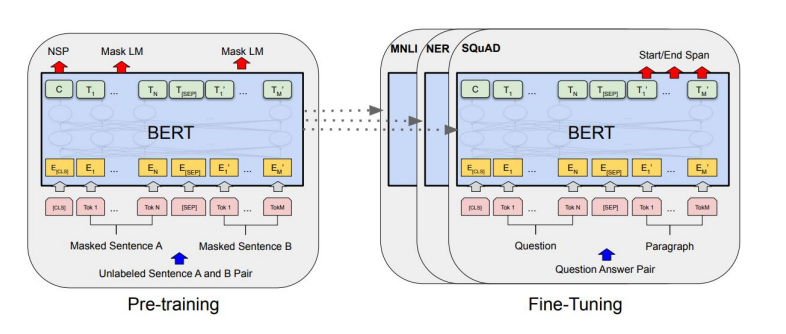
\includegraphics[width=0.9\textwidth]{bert}
\caption{Illustrazione riassuntiva del Pre-training e del Fine-Tuning di \acrshort{bert}. Source: Devlin et al. \cite{devlin2018bert}}\label{figura:bert}
\end{figure}

\acrshort{bert} ha guadagnato la maggior parte della sua popolarità grazie al fatto che può essere utilizzato in un'ampia varietà di compiti \acrshort{nlp} a valle senza grandi sforzi. Infatti, si presenta come un modello pre-addestrato su una grande quantità di dati e fornisce una rappresentazione generica del linguaggio che può essere messa a punto per affrontare qualsiasi problema (ad esempio, Question Answering, classificazione, Named-Entity Recognition, ecc.). La Figura \ref{figura:bert} mostra la procedura di pre-addestramento, la quale viene eseguita utilizzando due strategie:
\begin{enumerate}
    \item \textit{Masked Language Model}: per ogni sequenza di input, il 15\% dei token sono sostituiti dal token \texttt{[MASK]}. Successivamente, il modello viene addestrato per prevedere i valori originali dei token mascherati sfruttando il contesto sinistro e destro.
    \item \textit{Next Sentence Prediction (NSP)}: ogni sequenza di input è divisa in due parti separate dal token \texttt{[SEP]}. Poi, il 50\% delle sequenze viene modificato sostituendo la seconda parte con una casuale da un'altra sequenza. Infine, il modello è addestrato a distinguere sequenze positive e negative.
\end{enumerate}
L'alta qualità della rappresentazione del testo è ottenuta a spese di un elevato costo computazionale. Il modello \acrshort{bert} è originariamente disponibile in due versioni: \acrshort{bert} base (110M parametri) e \acrshort{bert} large (340M parametri). Queste dimensioni del modello richiedono elevate capacità di memoria e rendono la procedura di addestramento non accessibile a tutti. 
Per questo motivo, sono state proposte e rese disponibili diverse nuove versioni.

\section{Computer Vision}
Quando si lavora con le immagini, esse devono essere rappresentate in un formato comprensibile dalla macchina prima di qualsiasi elaborazione, la qualità delle caption finali dipende fortemente dalla qualità della rappresentazione dell'immagine.
\subsection{Object Detection}
Molti approcci di Image Captioning che hanno consentito il raggiungimento di risultati allo stato dell'arte hanno sfruttato l'Object Detection per effettuare la comprensione e l'estrazione delle feature delle immagini.

L'Object Detection è una tecnica di \acrlong{cv} che identifica e localizza degli oggetti all'interno di un'immagine. In particolare, il rilevamento degli oggetti viene effettuato tramite dei riquadri di delimitazione (bounding box) attorno agli oggetti rilevati e a ognuno di essi viene assegnata una classe (tag) che identifica l'oggetto identificato. La bounding box è di forma rettangolare e descrive la posizione spaziale di un oggetto tramite un vettore, il quale è composto dalle coordinate x e y dell'angolo superiore sinistro del rettangolo e da quelle dell'angolo inferiore destro.
Quando si usano i modelli di Object Detection la rappresentazione finale dell'immagine viene ottenuta tramite le rappresentazioni vettoriali dei vari oggetti che la compongono, solitamente queste feature vengono estratte da un layer intermedio del modello di detection.

\subsubsection{Faster R-CNN}\label{faster_rcnn_model}
Il modello di Object Detection più utilizzato è \acrshort{faster_rcnn} \cite{ren2015faster} (Figura \ref{figura:faster_rcnn}), il quale è una variante di \acrshort{rcnn} \cite{girshick2014rich} e di \acrshort{fast_rcnn} \cite{girshick2015fast}.
\acrshort{faster_rcnn} è stato progettato per identificare istanze di oggetti appartenenti a certe classi e per localizzarle tramite bounding box.
\begin{figure}[ht]
\centering
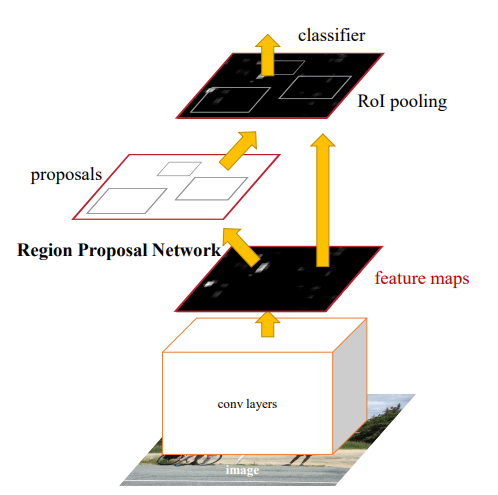
\includegraphics[width=0.5\textwidth]{faster_rcnn}
\caption{Illustrazione raffigurante l'architettura di \acrshort{faster_rcnn}. Source: Ren et al. \cite{ren2015faster}}\label{figura:faster_rcnn}
\end{figure}

Questo modello rileva gli oggetti tramite due fasi:
\begin{enumerate}
    \item \acrfull{rpn}: riceve come input un'immagine (di qualsiasi dimensione) e produce un insieme di proposte di oggetti. Questa componente è implementata tramite una piccola rete che viene fatta scorrere sulle feature estratte da un layer intermedio di una \acrshort{cnn} chiamata backbone. In ogni posizione spaziale la rete predice: un punteggio di objectness indipendente dalla classe e un raffinamento della bounding box chiamato anchor box, quest'ultimo ha una scala e una proporzione specifica. Con più anchor box di riferimento esistono più scale e proporzioni per la singola regione. Quindi, ciascuna regione viene mappata su ciascuna anchor box di riferimento, rilevando così oggetti a scale e proporzioni diverse. Usando la soppressione greedy non massima con una soglia di \acrfull{iou} vengono selezionate le proposte di regioni, le quali servono come input per la seconda fase;
    \item \acrfull{roipool}: usa il max pooling per convertire le feature all'interno di una qualsiasi regione di interesse in una piccola mappa di feature (viene effettuato un processo di quantizzazione sulle \acrshort{roi} ottenendo una granularità discreta delle mappe delle feature).
\end{enumerate}
Infine, i vettori di feature estratti utilizzando il \acrlong{roipool} vengono passati ad alcuni Fully Connected layer, l'ultimo di questi layer è suddiviso in due rami dove uno determina le classi e l'altro le bounding box degli oggetti rilevati.


Nonostante il modello \acrshort{faster_rcnn} non sia recente ed esistano modelli di Object Detection con performance superiori, risulta molto utilizzato nell'Image Captioning perché può essere utilizzato con backbone pre-addestrate sul dataset ImageNet (per esempio \acrshort{resnet} risulta essere la più popolare) e perché si basa sui layer convoluzionali, queste due caratteristiche permettono l'ottenimento di un migliore bias induttivo per la codifica delle informazioni visive delle regioni \cite{jiang2020defense}.

\subsection{Image Segmentation}
L'Image Segmentation oltre a predire la bounding box e l'etichetta di classe per ogni oggetto rileva anche la maschera di segmentazione, la quale permette di estrarre solo l'oggetto rilevato dall'immagine senza includere i pixel superflui dello sfondo.

Esistono tre tipologie principali di segmentazione:
\begin{enumerate}
\item \textbf{Semantic Segmentation}: assegna un'etichetta di classe a ogni pixel di un'immagine;
\item \textbf{Instance Segmentation}: rileva e delinea ogni istanza di oggetto con una maschera di segmentazione;
\item \textbf{Panoptic Segmentation} \cite{kirillov2019panoptic}: tratta sia le classi di tipo \textit{stuff} sia di tipo \textit{thing}, unificando i due tipi di segmentazione esposti precedentemente. 
Con stuff ci si riferisce a regioni amorfe e non numerabili di texture o materiale simile individuabili tramite la Semantic Segmentation (per esempio: sky, ground, grass, etc), mentre con thing ci si riferisce a oggetti numerabili individuabili tramite Instance Segmentation (per esempio people, animal, tool, etc).
L'attività di Panoptic Segmentation prevede l'assegnazione di un'etichetta semantica e di un ID di istanza per ciascun pixel di un'immagine, richiedendo la generazione di segmentazioni di scena dense, coerenti e complete.
\end{enumerate}
\begin{figure}[ht]
\centering
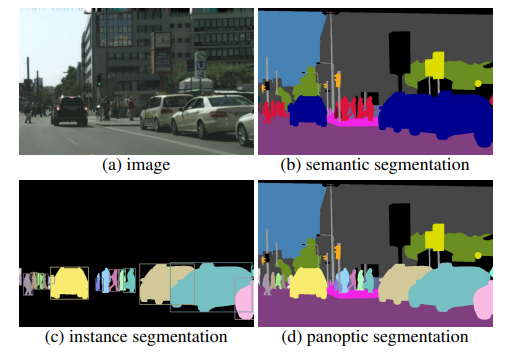
\includegraphics[width=0.8\textwidth]{segmentazioni}
\caption{Illustrazione in cui si può vedere la differenza di risultati tra le tipologie di Image Segmentation. Source: Kirillov et al. \cite{kirillov2019panoptic}}
\end{figure}
\newpage
\subsubsection{Mask R-CNN} \label{mask_section}
Un modello molto popolare di Instance Segmentation è \acrshort{mask_rcnn} \cite{he2017mask} (Figura \ref{mask_img}), il quale risulta molto interessate perché può essere visto come il miglioramento del modello di Object Detection \acrshort{faster_rcnn} (il quale si comporta bene nel contesto dell'Image Captioning, vedere sezione \ref{faster_rcnn_model}) con un ramo aggiuntivo che si occupa della predizione della maschera, questo ramo è una piccola \acrfull{fcn}.
\begin{figure}[ht]
\centering
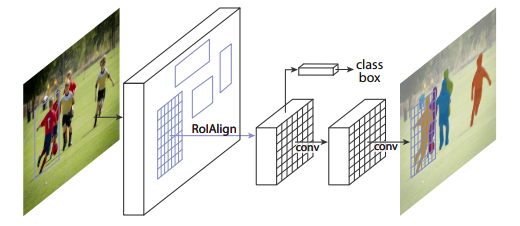
\includegraphics[width=0.8\textwidth]{mask_rcnn}
\caption{Illustrazione raffigurante l'architettura di \acrshort{mask_rcnn}. Source: He et al. \cite{he2017mask}}\label{mask_img}
\end{figure}


L'unica differenza tra i due modelli è la rimozione delle quantizzazioni utilizzate nel \acrshort{roipool}, le quali introducono disallineamenti tra le \acrshort{roi} e le feature estratte generando errori nella previsione di maschere accurate al pixel. Gli autori per risolvere questo problema hanno proposto un livello RoIAlign che rimuove la quantizzazione di \acrshort{roipool}, allineando correttamente le feature estratte con l'input, e usano l'interpolazione bilineare \cite{jaderberg2015spatial}, per calcolare i valori esatti delle feature di input in quattro posizioni regolarmente campionate in ogni bin \acrshort{roi} e aggregano il risultato (usando max o media).


\subsubsection{DETR} \label{detr_section}
\acrshort{detr} (\acrlong{detr}) \cite{carion2020end} è un modello di Object Detection che ha riscontrato successo nel task di Panoptic Segmentation. Questo modello è basato su Transformer e sulla bipartite matching loss per la previsione diretta del set.
\begin{figure}[ht]
\centering
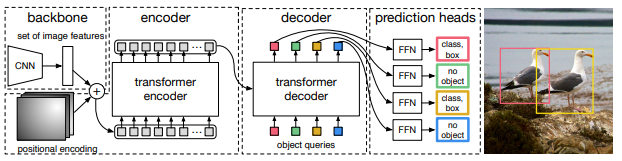
\includegraphics[width=0.85\textwidth]{detr}
\caption{Illustrazione raffigurante l'architettura di \acrshort{detr} per il task di Object Detection. Source: Carion et al. \cite{carion2020end}}\label{detr_img}
\end{figure}



L'architettura di DETR contiene tre componenti:
\begin{enumerate}
    \item Backbone \acrshort{cnn}: utilizzata per estrarre una rappresentazione compatta delle feature dell'immagine di input;
    \item Encoder-Decoder Transformer: 
    \begin{itemize}
        \item Transformer Encoder: riceve come input la rappresentazione precedentemente calcolata e genera delle codifiche più significative dell'immagine di input, contenenti informazioni posizionali.
        L'Encoder è composto da un modulo di multi-head self-attention e da una \acrfull{ffn}, inoltre agli input di ogni attention layer viene aggiunta una codifica posizionale (perché l'architettura del Transformer è invariante alle permutazioni);
        \item Transformer Decoder: riceve come input la memoria dell'Encoder e N object queries (sono le codifiche posizionali apprese). Trasforma gli N embedding di dimensione d usando il meccanismo multi-headed self- and encoder-decoder attention sfruttando la codifica ricevuta, questo si differenzia da quello standard perché permette la decodifica degli N oggetti in parallelo a ogni strato del decoder. Infine, gli embedding ottenuti, rappresentanti N codifiche di oggetti, vengono forniti come input alla rete \acrshort{ffn};
    \end{itemize}
    \item \acrfull{ffn}: riceve le N proposte ed effettua le predizioni finali del rilevamento.
\end{enumerate}

\acrshort{detr} ha avuto successo nella Panoptic Segmentation poiché può essere naturalmente esteso aggiungendo una mask head in cima agli output del decoder, riesce a trattare le classi stuff e thing in modo unificato.


\chapter{Stato dell'arte}\label{sec:Stato dell'arte}

L'Image Captioning è il compito di descrivere il contenuto visivo di un'immagine in linguaggio naturale e viene classificato nella letteratura come un problema image-to-sequence, il cui input è un insieme di pixel di un'immagine che viene codificato come uno o più vettori di feature. La rappresentazione ottenuta viene utilizzata da un ulteriore modello che determina una sequenza di parole.

La parte di comprensione dell'immagine è la componente più complessa poiché la descrizione potrebbe contenere qualsiasi aspetto visivo dell'immagine: può menzionare gli oggetti e i loro attributi, può considerare le caratteristiche della scena (per esempio, indoor/outdoor), o verbalizzare come le persone e gli oggetti nella scena interagiscono. Inoltre, la descrizione può anche riferirsi a oggetti che non sono raffigurati (per esempio, può fare riferimento a persone che aspettano un treno, anche quando il treno non è visibile perché non è ancora arrivato) e fornire conoscenze di base che non possono essere derivate direttamente dall'immagine (per esempio, la persona raffigurata è la Monna Lisa).


La comprensione dell'immagine è necessaria, ma non sufficiente per produrre una buona descrizione, in quanto quest'ultima deve essere completa ma concisa (parlare di tutte e solo le cose importanti nell'immagine) e deve essere formalmente corretta, cioè composta da frasi grammaticalmente ben formate. Da un punto di vista del \acrshort{nlp}, generare una tale descrizione è un problema di \acrfull{nlg}, il quale consiste nella trasformazione di una rappresentazione non linguistica in un testo leggibile dall'uomo. Classicamente, la rappresentazione non linguistica è una forma logica, una query o un insieme di numeri. Nella descrizione delle immagini, l'input è una rappresentazione dell'immagine che il modello di \acrshort{nlg} deve trasformare in frasi in linguaggio naturale.

Inoltre, il compito di descrizione può diventare ancora più impegnativo quando si tiene conto che le buone descrizioni sono spesso specifiche per l'utente. Per esempio, un critico d'arte richiederà una descrizione diversa da quella di un bibliotecario o di un giornalista, anche per la stessa immagine.
%L'obiettivo finale di questo task è quello di trovare una pipeline che elaborare un'immagine in ingresso, ne rappresenta il contenuto generando connessioni tra elementi visivi e testuali, infine la rappresentazione viene trasformata in una sequenza di parole che rispetta la fluidità del linguaggio.

\section{Metodi}
La letteratura esistente, in base all'approccio utilizzato, può essere suddivisa in due categorie principali \cite{bernardi2016automatic}: 
\begin{enumerate}
\item\textbf{Direct Generation models};
\item\textbf{Retrieval-based models};
\end{enumerate}
In questa sezione ci soffermeremo maggiormente sulla prima tipologia poiché è quella più utilizzata al giorno d'oggi ed è quella che ha consentito il raggiungimento dei risultati dello stato dell'arte.
\subsection{Direct Generation models}\label{directmodel}
Il task di Image Captioning è stato generalmente affrontato utilizzando questa tipologia di modelli, la quale si basa su pipeline composte da un codificatore visivo (\textbf{visual encoder}) che genera una rappresentazione dell'immagine e questa codifica viene utilizzata come input da un modello linguistico (\textbf{language model}) che si occupa della generazione del testo.
Nel corso degli anni, entrambi i componenti sono evoluti considerevolmente attraverso lo sfruttamento delle regioni delle immagini, attributi visivi, l'introduzione delle multi-modal connections, approcci fully-attentive e strategie di early-fusion tipo \acrshort{bert}. 
%Tuttavia, nonostante i risultati impressionanti, la ricerca sulla didascalia delle immagini non ha ancora raggiunto una risposta definitiva.
Inoltre, i modelli che sono stati sviluppati hanno affrontato questo problema concentrandosi su svariati aspetti poiché le persone hanno diversi stili di descrizione. Infatti, le didascalie delle immagini possono essere percettive, quando si concentrano su attributi visivi di basso livello; non visive, quando riportano informazioni implicite e contestuali; concettuali, quando descrivono l'effettivo contenuto visivo (per esempio entità visive e loro relazioni). Quest'ultimo è comunemente riconosciuto come l'obiettivo dell'Image Captioning, questa definizione comprende descrizioni che si concentrano su aspetti diversi e a vari livelli di dettaglio (per esempio, includendo o meno gli attributi, menzionando entità nominate o concetti di alto livello, descrivendo solo parti salienti o anche dettagli più fini). 

\subsubsection{Visual Encoder}
L'obiettivo di questo componente è quello di fornire una rappresentazione significativa del contenuto visivo dell'immagine e i vari approcci che sono stati utilizzati possono essere suddivisi nelle seguenti categorie \cite{stefanini2021show}: metodi \textbf{non-attentive} che si basano su feature globali estratte tramite una \acrshort{cnn}; metodi \textbf{additive attentive} che rappresentano il contenuto visivo usando griglie; metodi con \textbf{attention over visual regions} che estraggono regioni dall'immagine; metodi basati su grafi (\textbf{graph-based}) che aggiungono relazioni visive tra le regioni dell'immagine; metodi \textbf{self-attentive} che si basano sui Transformer.
\paragraph{Non-Attentive}
Questo è l'approccio più vecchio utilizzato per la codifica visiva dell'immagine ed è effettuata utilizzando l'attivazione di uno degli ultimi strati di una \acrshort{cnn} (escludendo la componente fully-connected). Questa tecnica è molto semplice e fornisce una rappresentazione compressa; tuttavia, le informazioni sono eccessivamente ristrette mancando di granularità, rendendo difficile per un modello di captioning la produzione di descrizioni dettagliate. 
\paragraph{Additive Attentive}
Questo approccio cerca di risolvere le criticità della tecnica precedente fornendo una rappresentazione più ricca di dettagli e per ottenere questo risultato utilizza l'additive attention \cite{bahdanau2014neural, stefanini2021show}.
Questo meccanismo viene utilizzato per connettere gli strati convoluzionali della \acrshort{cnn} con gli stati nascosti del language model. Questa tipologia di attention si basa solitamente su una single-layer \acrshort{ffn} che usa una hyperbolic tangent non-linearity per calcolare i pesi di attenzione, i quali indicano quanto una porzione dell'immagine è importante per la predizione della caption.
Quindi, l'immagine viene trattata come una griglia di elementi ottenuta dall'output di uno strato convoluzionale di una \acrshort{cnn}, gli elementi di questa griglia sono utilizzati per calcolare un peso che specifica l'importanza relativa di quell'elemento per generare la parola successiva.
%Formalmente dati due insiemi di vettori ${x_1, ..., x_n}$ (elementi della griglia) e ${h_1, ..., h_m}$ (stati nascosti del modello linguistico), il punteggio di attenzione additiva tra il vettore $h_i$ e il vettore $x_j$ è calcolato come: 
%\begin{equation}
%	f_{att}(h_i, x_j) = W_3^T \cdot tanh(W_1 \cdot h_i + W_2 \cdot x_j) 
%\end{equation}
%dove $W_1$ e $W_2$ sono matrici di pesi, mentre $W_3$ è un vettore di pesi per effettuare una combinazione lineare. Infine, viene applicata una funzione di softmax per ottenere una distribuzione di probabilità p($x_j|h_i$) che specifica la rilevanza della codifica di $x_j$ per $h_i$.

\paragraph{Attention Over Visual Regions}
%Questa tecnica utilizza un'intuizione derivante dalle neuroscienze, la quale suggerisce che il cervello umano utilizza un processo di ragionamento top-down con un flusso bottom-up di segnali visivi. Il termine top-down consiste nel prevedere utilizzando le conoscenze pregresse e induttive. Mentre, con il termine bottom-up ci si riferisce all'estrazione di stimoli visivi.
%Nel contesto dell'Image Captioning la fase bottom-up è effettuata solitamente tramite un rilevatore di oggetti che identifica le regioni più rilevanti di un'immagine; successivamente viene utilizzato un meccanismo top-down che filtra e utilizza i risultati ottenuti precedentemente per generare la frase finale. 
Questa tecnica sfrutta un modello di Object Detection incaricato di proporre le regioni più rilevanti dell'immagine e ogni regione viene rappresentata tramite un vettore di feature convoluzionali, solitamente estratte da un layer intermedio del modello di detection.
\paragraph{Graph-based}
Questa tecnica migliora la codifica precedente utilizzando un grafo, dove i nodi sono le regioni dell'immagine e gli archi rappresentano le relazioni semantiche e spaziali tra le regioni.
\paragraph{Self-Attentive}
Questa tecnica si basa sul meccanismo di self-attention \cite{vaswani2017attention} dei Transformer, in cui ogni elemento di un insieme di elementi è connesso a tutti gli altri e viene utilizzato per calcolare una rappresentazione raffinata dello stesso insieme di elementi tramite connessioni residue. Ad esempio, può essere utilizzato per codificare le relazioni tra le feature estratte tramite un modello di Object Detection.
%Formalmente la self-attention si basa su un operatore di attenzione moltiplicativo che utilizza tre insiemi di vettori: un insieme di vettori query Q contente $n_q$ valori, un insieme di vettori chiave K e un insieme di vettori valore V, entrambi contenti $n_k$ elementi. 
%Successivamente questi vettori vengono combinati per determinare un vettore di output calcolato come somma pesata dei valori, dove il peso assegnato a ciascun valore è calcolato da una funzione di compatibilità tra la query e la chiave corrispondente. Viene usata la formula seguente:
%\begin{equation}
%Attention(Q,K,V) = softmax(\frac{Q \cdot K^T}{\sqrt{d_k}}) \cdot V
%\end{equation}
%dove $d_k$ è un vettore di scalari rappresentanti la dimensione del vettore chiave.


\subsubsection{Language Models}
L'obiettivo di un modello linguistico è quello di predire la probabilità che una data sequenza di parole si verifichi in una frase. Quindi formalmente data una sequenza di n parole un modello linguistico assegna una probabilità $P(y_1, y_2, ..., y_n|X)$ alla sequenza tramite:
\begin{equation}
\label{eqn:formula_caption}
P(y_1, y_2, ..., y_n|X) = \prod_{i=1}^{n}P(y_i|y_1, y_2, ..., y_{i-1},X)
\end{equation}
dove X rappresenta la codifica visuale ottenuta dal visual encoder sulla quale il modello linguistico è condizionato. Questi modelli sono auto regressivi poiché ogni parola dipende da quelle precedenti e di solito decidono quando terminare la frase emettendo un token speciale di fine sequenza.
I vari approcci che sono stati utilizzati possono essere suddivisi nelle seguenti categorie \cite{stefanini2021show}: \textbf{\acrshort{rnn}-based}, \textbf{\acrshort{cnn}-based}, \textbf{Transformer-based}, \textbf{Image-text early-fusion} (\acrshort{bert}-like) e \textbf{Non-autoregressive}.
I vari modelli di decodifica visiva visti precedentemente vincolano le descrizioni generate, poiché si basano su un insieme predefinito di classi semantiche di scene, oggetti, attributi e regioni. Inoltre, i modelli di decodifica devo ottenere un'ottima accuratezza nel rilevamento per ogni classe semantica, un presupposto che non è sempre soddisfatto nella pratica e che di conseguenza può peggiorare la qualità finale delle caption.
\paragraph{\acrshort{rnn}-based}
Questo approccio usa le reti \acrfull{rnn} per generare la caption, questa tipologia di rete neurale si è comportata molto bene poiché il linguaggio ha una struttura sequenziale e quindi è adatta a trattare la generazione di frasi; la \acrfull{lstm} è stata l'architettura più utilizzata. Quindi la codifica visiva viene utilizzata come stato nascosto iniziale di una \acrshort{rnn}, che poi genera la didascalia in uscita. A ogni passo temporale, una parola è prevista applicando una funzione di attivazione sulla proiezione dello stato nascosto in un vettore della stessa dimensione del vocabolario utilizzato, che ne genera una distribuzione di probabilità.
Inoltre, sono state utilizzate anche versioni più avanzate come per esempio strutture \acrshort{lstm} multistrato (che aumentano la capacità di catturare relazioni di ordine superiore) o architetture che usano il meccanismo di attention, dove la predizione della parola è condizionata solo da alcune parti diverse dell'immagine che sono quelle considerate più importanti. In quest'ultimo caso la rete apprende dove deve prestare attenzione nell'input visivo per predire ogni elemento della sequenza di output.
Questi modelli sono lenti da addestrare e hanno difficoltà nel mantenere dipendenze a lungo termine.
\paragraph{\acrshort{cnn}-based}
Questo approccio fornisce le feature visuali a un modello \acrshort{cnn} che si occupa della predizione delle didascalie. Il modello convoluzionale opera su tutte le parole in parallelo durante l'addestramento e sequenzialmente in inferenza, le convoluzioni sono mascherate a destra per evitare che il modello utilizzi le informazioni di token futuri.
Questa tipologia di modelli permette il training parallelo ma non ha acquisito molta popolarità a causa delle performance insoddisfacenti.
\paragraph{Transformer-based}
Questo approccio si basa sull'architettura del decoder usato dal modello Transformer che può essere applicato in questo contesto perché la generazione delle didascalie può essere visto come un problema sequence-to-sequence.
Il decodificatore Transformer esegue un'operazione di self-attention mascherata, la quale sostituisce alcune parole con un token particolare \texttt{[MASK]} con l'obiettivo di acquisire un processo di generazione unidirezionale, seguita da un'operazione di cross-attention nella quale le parole rappresentano le query e i risultati dell'ultimo strato di codifica rappresentano le chiavi e i valori. Successivamente le query, le chiavi e i valori vengono combinati e la rappresentazione risultante viene elaborata da una rete neurale composta da layer feed-forward, i quali producono la distribuzione di probabilità sul vocabolario delle parole che andranno a comporre la didascalia finale.
\paragraph{Image-text early-fusion}
Questo approccio utilizza un'architettura ispirata a \acrshort{bert} \cite{devlin2018bert} nella quale il modello riceve input composti da una parte visiva e da una parte testuale, successivamente le due modalità sono fuse insieme nei layer iniziali. Questa tipologia permette ai layer che si occupano del testo di essere inizializzati con parametri pre-addestrati appresi da corpus testuali. Inoltre, recentemente alcuni approcci pre-addestrano questi modelli su grossi insiemi di dataset che prevedono sia componenti visuali che testuali. Ad esempio, questa tecnica può essere usata quando il visual encoder estrae oltre alle feature visuali anche feature testuali che descrivono il contenuto dell'immagine (per esempio attributi testuali o i nomi degli oggetti presenti).
\paragraph{Non-autoregressive}
Questi approcci sfruttano il parallelismo offerto dai Transformer riducendo drasticamente i tempi di inferenza. Questi modelli sono composti da un certo numero di stadi di generazione diversi, dove tutte le parole sono predette in parallelo e raffinate piano piano a ogni stadio. Inoltre, sfruttano tecniche di \acrlong{rl} per migliorare i risultati finali. Questi modelli trattano il processo di generazione come un cooperative multi-agent reinforcement system, dove le posizioni delle parole nella sequenza finale sono viste come agenti che imparano a massimizzare cooperativamente una ricompensa a livello di frase. Infine, è prevista una distillazione della conoscenza sui dati non etichettati e una fase di post-elaborazione per rimuovere i token consecutivi identici.

\subsubsection{Esempi}
Karpathy et all. \cite{karpathy2015deep} usano una \acrshort{rcnn} per rilevare gli oggetti nelle immagini, il modello che usano è pre-addestrato su ImageNet e messo a punto sulle 200 classi dell'ImageNet Detection Challenge. Per ottenere la rappresentazione dell'immagine in uno spazio h-dimensionale usano una \acrshort{cnn} che effettua una codifica sui primi 19 oggetti rilevati all'interno dell'immagine (ordinati in base allo score decrescente) e all'intera immagine. Utilizzano word2vec \cite{mikolov2013efficient} per effettuare la codifica di ogni parola della caption in vettori di dimensionalità 300, successivamente queste rappresentazioni vengono utilizzate come input per una \acrfull{brnn} la quale effettua una codifica nello stesso spazio h-dimensionale. Successivamente viene utilizzato un \acrfull{mrf} che assegna le parole delle caption alle regioni dell'immagine estratte tramite \acrshort{rcnn} creando dei frammenti della caption.
Quindi l'output consiste in un insieme composto dalle regioni dell'immagine annotate con segmenti di testo della caption di partenza e dall'immagine di partenza che avrà come segmento l'intera caption.
Infine, viene allenata una multimodal \acrshort{rnn} per predire il frammento di testo data la regione o la caption intera data l'immagine originale. %Per la decodifica è stato utilizzato il beam search con il parametro K pari a 7.

You, Jin et all. \cite{you2016image} usano una \acrshort{cnn} per estrarre la rappresentazione vettoriale dell'immagine e tramite dei rilevatori estraggono degli attributi visuali, i quali vengono rappresentati in uno spazio vettoriale tramite word2vec. Infine, le informazioni precedentemente estratte vengono utilizzate come input da una \acrshort{rnn} con attention che produce la caption finale. Gli attributi visuali sono estratti tramite un modello \acrshort{fcn} che è stato allenato a predire degli attributi data un'immagine (classificazione multiclasse), per il training hanno costruito un insieme di attributi visuali prendendo le 1000 parole più comuni provenienti dalle caption di allenamento. Sulle caption è stato effettuato preprocessing selezionando solo i nomi, i verbi e gli aggettivi più significativi.

Xu et all. \cite{xu2015show} dividono l'immagine in L parti e per ciascuna di esse estraggono una rappresentazione vettoriale usando una \acrshort{cnn}, la codifica ottenuta viene usata come input per una \acrshort{lstm}.
Il language model utilizza un meccanismo di attention spaziale che genera una rappresentazione interna dinamica delle parti più importanti dell'immagine al tempo t, la quale aiuta la predizione della parola nello stesso lasso temporale t. Il meccanismo utilizzato, per ogni posizione I dell'immagine, genera un peso positivo che può essere interpretato sia come la probabilità che la posizione I sia il posto giusto su cui concentrarsi per produrre la parola successiva, o come l'importanza relativa da dare alla posizione I nel fonderla insieme ad altre porzioni. Il peso di ogni posizione è calcolato da un modello di attenzione implementato utilizzando un perceptron multistrato condizionato sullo stato nascosto precedente $h_{t-1}$ del modello \acrshort{lstm}. Infine, questi pesi sono utilizzati per combinare le rappresentazioni delle posizioni dell'immagine insieme generando una rappresentazione interna che viene utilizzata per la predizione della parola al tempo t.

Liu et all. \cite{liu2021cptr} sostituiscono il modello \acrshort{cnn} con un modello Transformer per effettuare la decodifica dell'immagine di input, trattando il problema di Image Captioning come un task sequence-to-sequence.
Ridimensionano e dividono l'immagine originale in una sequenza di patch per adattarsi alla forma di input del Transformer, appiattiscono ogni suddivisione e trasformano i risultati in una sequenza monodimensionale. Successivamente usano uno strato di embedding lineare per mappare le sequenze in uno spazio latente, nel quale viene aggiunto un embedding di posizione monodimensionale imparabile dalle caratteristiche delle patch. Le sequenze precedentemente calcolate sono utilizzate come input da un codificatore Transformer (modello \acrshort{vit}) che fornisce la rappresentazione visuale finale.
La codifica precedentemente ottenuta viene utilizzata come input da un decodificatore Transformer che si occupa della predizione della caption.
Questo approccio evita totalmente l'operazione di convoluzione che non consente alle \acrshort{cnn} di codificare correttamente il contesto globale, questa limitazione può essere risolta allargando il campo ricettivo gradualmente man mano che gli strati di convoluzione vanno più in profondità. Infine, il codificatore utilizzato può sfruttare le dipendenze a lungo raggio tra le patch sequenzializzate fin dall'inizio tramite il meccanismo di self-attention.

Anderson et all. \cite{anderson2018bottom} usano un modello di attenzione bottom-up implementato tramite un modello di Object Detection chiamato \acrshort{faster_rcnn} con backbone \acrshort{resnet}-101 (entrambi pre-addestrati su ImageNet), prendono l'output finale del modello ed eseguono la soppressione non massima per ogni classe di oggetto usando una soglia \acrshort{iou}. Successivamente selezionano tutte le regioni in cui la probabilità di rilevamento di una qualunque classe supera una soglia di fiducia e per ognuna di esse estraggono un vettore di feature, rappresentante la feature convoluzionale media della regione estratta da un layer interno di \acrshort{faster_rcnn}.
Il modello di detection è stato allenato sui dati di Visual Genome (dataset che per ogni oggetto della detection contiene anche attributi visuali che lo descrivono) e per aiutare l'apprendimento di feature significative aggiungono un output di allenamento addizionale per predire degli attributi visuali per ogni regione (oltre alle classi degli oggetti). 
Infine, oltre al modello precedente usano una architettura top-down implementata tramite una \acrshort{lstm} con attention, il cui input consiste nell'output precedente del modello linguistico concatenato con un vettore rappresentante la media delle codifiche delle regioni estratte tramite Object Detection e dalla parola precedentemente predetta. %, per decodificare l'output usano il beam search.

Zhou et all. \cite{zhou2020unified} \label{unified_model} hanno creato un \acrlong{vlp} Transformer (\acrshort{vlp}) allenato su un grosso dataset composta da 3 milioni di coppie immagine e testo associato, creando un modello pre-addestrato sul quale poi verrà effettuato fine-tuning per eseguire l'Image Captioning.
Gli autori hanno utilizzato un modello di Object Detection per estrarre N regioni da ogni immagine, le quali sono state codificate in un vettore sfruttando un layer intermedio del modello di detection. Le rappresentazioni ottenute tramite detection sono state arricchite, concatenando le coordinate dell'angolo superiore sinistro e inferiore destro della bounding box, ed è anche stato aggiunto un valore rappresentante l'area relativa della regione. Invece, le parole del testo associato sono codificate utilizzando il word embedding di \acrshort{bert} (per maggiori dettagli vedere la sezione \ref{bert_section}). Il Transformer viene pre-addestrato utilizzando la funzione di perdita di \acrshort{bert} e riceve come input la codifica dell'immagine (effettuata tramite regioni) e dei testi associati (che deve imparare a predire). 
Infine, il modello precedentemente creato viene addestrato sul task specifico di Image Captioning (fine-tuning) ricevendo come input le regioni dell'immagine e la didascalia da predire.


Wang et all. \cite{wang2020visual} hanno sviluppato una variante della \acrshort{rcnn} chiamata Visual Commonsense \acrshort{rcnn} (VC \acrshort{rcnn}) che usa l'intervento causale come funzione obiettivo e viene utilizzata come estrattore di feature regionali, la quale può essere accompagnata da un qualsiasi language model.
L'intervento causale è definito come $P(Y|do(X)) = \sum\limits_{z} P(Y|X,z) \cdot P(z)$, dove X è l'oggetto che causa la predizione del oggetto Y, mentre z sono i confonditori che sono principalmente oggetti (bias osservabile nell'immagine) e influenzano sia X che Y. Questa tecnica si basa sull'idea che i sistemi di computer vision odierni sono bravi a dire "cosa" (per esempio: classificazione) e "dove" (per esempio: rilevamento e tracciamento), ma pessimi nel sapere "perché". Questo non significa semplicemente chiedere ragioni visive, ma significa anche chiedere ragioni di senso comune di alto livello (common sense) catturando un contesto non locale che potrebbe non essere presente nell'immagine.


Rennie et all. \cite{rennie2017self} utilizzano un modello \acrshort{cnn} per estrarre la rappresentazione vettoriale dell'immagine e successivamente sul vettore ottenuto effettuano una proiezione lineare. Mentre la caption viene codificata tramite la tecnica one hot encoding, sul vettore risultante viene effettuata una proiezione lineare per ottenere la stessa dimensione della rappresentazione finale dell'immagine.
Le rappresentazioni ottenute vengono fornite come input a un modello \acrshort{lstm}, il quale viene allenato per la predizione delle caption.
I modelli generativi di Image Captioning sono tipicamente addestrati per massimizzare la probabilità della prossima parola ground-truth data la parola ground-truth precedente usando la back-propagation. Tuttavia, questo approccio crea una discrepanza tra l'addestramento e il test, poiché durante la valutazione il modello usa le parole generate in precedenza dalla distribuzione di probabilità per prevedere la parola successiva \cite{ranzato2015sequence}. Questo genera bias di esposizione che si traduce in un accumulo di errori durante la generazione al momento del test, poiché il modello non è mai stato esposto alle sue stesse predizioni.
Inoltre, i modelli linguistici sono solitamente allenati utilizzando la Cross Entropy loss la quale si differenzia molto dalle metriche utilizzate in fase di test, poiché durante la valutazione si utilizzano metriche \acrshort{nlp} discrete e non differenziabili. Idealmente i modelli di Image Captioning dovrebbero essere addestrati a ottimizzare direttamente le metriche per il compito da svolgere.
Recentemente è stato dimostrato che entrambi i problemi di esposizione e di metrica del compito non differenziabile possono essere affrontati incorporando tecniche di apprendimento per rinforzo.
Gli autori \cite{rennie2017self} hanno sviluppato un nuovo approccio di ottimizzazione basato sul \acrlong{rl} chiamato \textbf{\acrfull{scst}} \label{scst} che è una variante di REINFORCE e può essere utilizzato per il training del modello linguistico risolvendo i problemi evidenziati precedentemente.
Quindi, il modello linguistico può essere visto come un "agente" che interagisce con un "ambiente" esterno (parole e caratteristiche dell'immagine); mentre i parametri del modello $\theta$ definiscono una politica $p_\theta$, la quale risulta in una "azione" che è la previsione della parola successiva.
Dopo ogni azione, l'agente aggiorna il suo "stato" interno (celle e stati nascosti del modello \acrshort{lstm}, pesi di attenzione, ecc.) e dopo aver generato il token di fine sequenza l'agente osserva una "ricompensa" r. La ricompensa è calcolata da una metrica di valutazione che confronta la sequenza generata con le corrispondenti sequenze ground-truth, l'obiettivo dell'addestramento è quello di minimizzare la ricompensa attesa negativa.

%appartiene a una classe speciale di algoritmi di Reinforcement Learning chiamati algoritmi Policy Gradient e la sua implementazione prevede un modello che prende uno stato come input e genera la probabilità di intraprendere un'azione come output. Una politica è essenzialmente una guida per l'agente che gli dice quale azione intraprendere in ogni stato. La politica viene quindi ripetuta e leggermente modificata a ogni passaggio fino a quando non si ottiene una politica che risolva l'ambiente.
\textbf{REINFORCE} \cite{rennie2017self} è un algoritmo di \acrlong{rl} e si basa sull'osservazione che il gradiente atteso di una funzione di ricompensa non differenziabile può essere approssimato usando un singolo campione Monte-Carlo $w_s$ da $p_\theta$, per ogni esempio di allenamento nel minibatch. Il gradiente dato da REINFORCE può essere generalizzato per calcolare la ricompensa associata a un valore di azione rispetto a una ricompensa di riferimento o baseline b. Quest'ultima può essere una funzione arbitraria, purché non dipenda dall'azione. La baseline non cambia il gradiente atteso, ma soprattutto può ridurre la varianza della stima del gradiente. 

L'idea centrale dell'approccio \textbf{\acrshort{scst}} è di basare l'algoritmo REINFORCE sulla ricompensa ottenuta dal modello corrente sotto l'algoritmo di inferenza usato al momento del test (invece REINFORCE stima una "linea di base" per normalizzare le ricompense e ridurre la varianza). Quindi, utilizza l'output del proprio algoritmo di inferenza a test-time per normalizzare le ricompense che sperimenta. Il gradiente della ricompensa negativa di un campione $w^s$ ottenuto dal modello rispetto alle attivazioni softmax al time-step t diventa:
\begin{equation*}
\frac{\partial L(\theta)}{\partial	s_t} = (r(w^s) - r(w'))(p_\theta(w_t|h_t) - 1_{w_t^s})
\end{equation*}
dove r(w') è la ricompensa ottenuta dal modello corrente sotto l'algoritmo di inferenza usato al momento del test. Di conseguenza, i campioni del modello che restituiscono una ricompensa più alta di w' saranno "spinti in alto", o aumentati in probabilità, mentre i campioni che risultano in una ricompensa più bassa saranno soppressi.
Quindi \acrshort{scst} usa direttamente la vera metrica di valutazione a livello di sequenza ed evita lo scenario di dover imparare una stima (dipendente dal contesto) delle ricompense future previste come baseline. 


Yao et all. \cite{yao2018exploring} sfruttano le correlazioni e le interazioni tra gli oggetti per descrivere un'immagine, le quali sono rappresentate tramite triple (subject-predicate-object). %La loro identificazione è molto difficile perché gli oggetti possono essere con un'ampia gamma di scale, in posizioni arbitrarie e provenienti da diverse categorie.
Gli autori hanno introdotto un'architettura innovativa chiamata Graph Convolutional Networks + Long Short-Term Memory (\acrshort{gcn}+\acrshort{lstm}), la quale prevede un modello di Object Detection che propone un insieme di regioni salienti dell'immagine.
Le regioni precedentemente estratte vengono utilizzate per costruire un grafo semantico con archi diretti, dove un nodo rappresenta una regione e l'arco denota la relazione (predicato) tra ogni coppia di regioni; quest'ultima è predetta da un rilevatore di relazioni semantiche (modello di classificazione) e può essere un'azione o un'interazione. Successivamente viene definito il grafo spaziale che è costruito da nodi rappresentanti le regioni e gli archi tra i nodi rappresentano la relazione geometrica relativa. 
Tramite una \acrfull{gcn} vengono arricchite le rappresentazioni delle regioni includendo le relazioni visive del grafo semantico e spaziale. Infine, le rappresentazioni delle regioni consapevoli delle relazioni apprese sono utilizzate come input da un modello \acrshort{lstm}, composto da due layer con attention, che genera la didascalia. 

%Nella fase di inferenza, per combinare le uscite dei modelli linguistici, viene calcolata la media lineare delle distribuzioni di probabilità delle parole dei decodificatori ad ogni passo temporale e l'output consiste nella parola con la probabilità più alta; quest'ultima viene usata come parola di input per entrambi i decodificatori al passo temporale successivo. 
%Usano la fusione tardiva per combinare due modelli linguistici LSTM che sono addestrati indipendentemente su modalità diverse. Tuttavia, a causa della natura ricorrente intrinseca e del complesso meccanismo di funzionamento, le RNN non riescono a esplorare le due modalità complementari simultaneamente.


%non tutte le parole della didascalia hanno segnali visivi corrispondenti
Li et all. \cite{li2019entangled} cercano di risolvere il problema dei meccanismi di attenzione che sono difficili da identificare in segnali visivi equivalenti, specialmente quando si predicono parole altamente astratte e relazioni complesse. Questo fenomeno è noto come gap semantico tra visione e linguaggio. Questo problema può essere superato fornendo attributi semantici omologhi al linguaggio.
Il modello utilizzato dagli autori si chiama ETA-Transformer, l'architettura generale segue il paradigma encoder-decoder e riceve come input delle feature visive e testuali.
Le caratteristiche visive sono composte dalle regioni estratte tramite un modello di Object Detection, le quali sono rappresentate tramite un layer intermedio e a queste feature viene aggiunta l'immagine di input a grandezza naturale codificata con il modello VGG-16.
Le caratteristiche testuali sono rappresentate da attributi semantici estratti tramite un rilevatore di attributi che riceve come input l'immagine codificata tramite VGG-16.
L'architettura utilizzata per effettuare Image Captioning prevede un dual-way encoder che mappa gli input originali in rappresentazioni altamente astratte, poi il decoder incorpora le informazioni multimodali simultaneamente per generare la didascalia parola per parola.
Il dual-way encoder consiste in due sotto-codificatori Transformer, i quali hanno la stessa struttura composta da layer con self-attention seguiti da una \acrfull{fnn} che consiste in due trasformazioni lineari con un'attivazione \acrshort{relu} nel mezzo.
La struttura descritta precedentemente può essere usata per codificare sia le caratteristiche visive che semantiche. Il sotto-codificatore riceve come input le caratteristiche visive, mappate tramite una trasformazione lineare, e gli attributi semantici, rappresentati tramite one-hot encoding e trasformati da uno strato di embedding (il codificatore e il decodificatore condividono gli stessi embedding).
Le informazioni codificate vengono utilizzate dal decodificatore Transformer (anch'esso composto da due sotto architetture) per produrre la caption finale.
Questo decodificare aggiunge un modulo ETA (Entangled Attention) e un modulo GBC (Gated Bilateral Controller) tra il layer di self-attention e il layer feed-forward, che gli permettono di eseguire l'attenzione sulle uscite visive e semantiche del codificatore simultaneamente. 
ETA esegue il meccanismo di attention in modo intrecciato sulla rappresentazione visuale e semantica sfruttando le connessioni residue tra le due componenti (le informazioni visuali vengono utilizzate dal meccanismo di attention della componente semantica e viceversa).
Il GBC si occupa dell'integrazione delle rappresentazioni generate precedentemente ed è composto da un layer Fully connected con funzione di attivazione sigmoid e da un meccanismo di gating bilaterale che controlla: la propagazione delle informazioni visive, la propagazione dell'informazione semantica e la generazione della caption.

\subsection{Retrieval-based models}
Questo gruppo di modelli considera il task come un problema di retrieval. Cioè, la creazione di una descrizione per una nuova immagine consiste nella ricerca di immagini simili a quella di interesse in un database. Successivamente, viene costruita una caption per la nuova immagine basata sulle descrizioni dell'insieme di immagini simili che sono state recuperate. La caption può essere generata semplicemente riutilizzando la descrizione dell'immagine più simile recuperata (trasferimento), o sintetizzando una nuova descrizione basata sulle caption dell'insieme di immagini simili (per esempio, seguendo delle regole o utilizzando un modello linguistico). I modelli basati sul retrieval possono essere ulteriormente suddivisi in base al tipo di approccio che utilizzano per rappresentare le immagini e per calcolare la somiglianza \cite{bernardi2016automatic}. Il primo sottogruppo di modelli usa uno spazio visivo per recuperare le immagini (\textbf{Retrieval in Visual Space}), mentre il secondo sottogruppo usa uno spazio multimodale (\textbf{Retrieval in Multimodal Space}) che rappresenta immagini e testo insieme.

\subsubsection{Retrieval in Visual Space}\label{retreivalvisualspace}
Questi metodi si pongono il problema di generare automaticamente la descrizione di un'immagine recuperando immagini simili alla query (cioè, la nuova immagine da descrivere). Quindi, questi sistemi sfruttano la somiglianza nello spazio visivo per trasferire le descrizioni alle immagini di interrogazione. Rispetto ai modelli che generano direttamente le descrizioni (Sezione \ref{directmodel}), i modelli di retrieval richiedono tipicamente una grande quantità di dati di allenamento per fornire descrizioni rilevanti.

Questi approcci seguono tipicamente una pipeline composta da tre fasi principali:
\begin{enumerate}
\item Rappresentare l'immagine data con specifiche feature visive;
\item Recuperare un sottoinsieme di immagini candidate dall'insieme di allenamento, sfruttando una misura di somiglianza nello spazio delle feature utilizzate;
\item Riqualificare le descrizioni delle immagini candidate utilizzando ulteriormente le informazioni visive e/o testuali contenute nel sottoinsieme identificato, o in alternativa combinare frammenti delle descrizioni candidate secondo certe regole o schemi;
\end{enumerate}



\subsubsection{Retrieval in Multimodal Space}
Questi metodi proiettano la generazione della descrizione dell'immagine di nuovo come un problema di retrieval, ma da uno spazio multimodale e l'approccio può essere caratterizzato dalle seguenti fasi:
\begin{enumerate}
\item Imparare uno spazio multimodale comune per i dati visivi e testuali utilizzando un set di allenamento di coppie immagine-descrizione;
\item Data un'immagine query, usare lo spazio di rappresentazione congiunto per eseguire il cross-modal (image–sentence) retrieval.
\end{enumerate}
Quindi, in contrasto con i modelli di retrieval che lavorano su uno spazio visivo, dove il recupero unimodale delle immagini è seguito da una classificazione delle descrizioni recuperate, in queste tecniche le feature delle immagini e delle frasi sono proiettate in uno spazio multimodale comune. Successivamente, lo spazio multimodale viene utilizzato per recuperare le caption per una data immagine. Il vantaggio di questo approccio è che permette modelli bidirezionali, cioè lo spazio comune può anche essere usato per l'altra direzione recuperando l'immagine più appropriata per una frase di query.

\subsubsection{Esempi}

Il metodo di Gupta et al. \cite{gupta2012choosing} recupera immagini visivamente simili utilizzando semplici istogrammi di colore RGB e HSV, descrittori Gabor e Haar, descrittori GIST e SIFT come estrattori di feature delle immagini. Successivamente, le descrizioni candidate sono segmentate in frasi nella forma: (subject, verb), (subject, prep, object), (verb, prep, object), (attribute, object), ecc. Le componenti che descrivono meglio l'immagine di input sono determinate secondo un modello di probabilità congiunto basato sulla somiglianza dell'immagine e sui conteggi di ricerca di Google. L'immagine è rappresentata da triplette nella forma {((attribute1, object1), verb), (verb, prep, (attribute2, object2)), (object1, prep, object2)}. Alla fine, la descrizione viene generata usando le tre triplette con il punteggio più alto basandosi su un template fisso. Per aumentare la qualità delle descrizioni, gli autori applicano anche l'aggregazione sintattica e alcune regole di raggruppamento di soggetti e predicati prima della fase di generazione.

Devlin et al. \cite{devlin2015language} utilizzano un modello \acrshort{cnn} come descrittore globale dell'immagine ed eseguono il retrieval tramite k-nearest neighbor per determinare le immagini dal set di allenamento che sono visivamente simili all'immagine della query. La somiglianza delle descrizioni è calcolata basandosi sul punteggio di sovrapposizione di n-grammi tra le descrizioni, in questo modello la caption di output corrisponde alla descrizione con la più alta sovrapposizione media di n-grammi con le altre candidate.

Socher et al. \cite{socher2014grounded} usano reti neurali per costruire rappresentazioni vettoriali di frasi e immagini che vengono poi mappate in uno spazio comune di embedding.  Quindi, le rappresentazioni di immagini e parole sono apprese nelle loro singole modalità e infine mappate in uno spazio multimodale comune. In particolare, usano una DT-RNN (Dependency Tree Recursive Neural Network) per comporre i vettori linguistici e per astrarre dall'ordine delle parole e dalla differenza sintattica che sono semanticamente irrilevanti, fornendo embedding di parole con 50 valori.
DT-RNN riceve come input una rappresentazione della frase di input s come una lista ordinata di coppie (parola, vettore): s = $(( w_1, x_{w_1}), . . . , (w_m, x_{w_m}))$, dove $x_{w_i}$ indica la colonna i-esima della matrice di embedding  X. Successivamente, la sequenza di parole $(w_1, . . . , w_m)$ viene analizzata dal parser delle dipendenze e il risultato viene utilizzato per costruire un albero delle dipendenze d di una frase s. La rappresentazione finale è ottenuta moltiplicando gli embedding dei nodi foglia con delle matrici di peso, le quali dipendono dalla posizione del nodo rispetto alla radice e dalle relazioni semantiche fornite dal parser delle dipendenze.
Le immagini sono codificate tramite un modello \acrshort{cnn} addestrato sui dati di ImageNet e viene preso l'output dell'ultimo strato convoluzionale. Le due tipologie di rappresentazioni sono proiettate in uno spazio multimodale comune attraverso una funzione obiettivo max-margin.
Durante l'inferenza l'immagine viene mappata nello spazio vettoriale e successivamente viene cercata la descrizione testuale di output trovando i vettori di frasi vicini nello spazio di incorporazione multimodale (classifica basata sui prodotti interni).

\subsection{Algoritmi di decodifica}\label{algoritmi_decodifica}
I modelli linguistici generano una distribuzione di probabilità su ogni parola del vocabolario per ogni parola della didascalia finale ed esistono algoritmi di decodifica che usano questa distribuzione di probabilità per generare la caption più probabile.
La decodifica della sequenza di output implica la ricerca di tutte le possibili sequenze di output in base alla loro probabilità. La dimensione del vocabolario spesso è elevata e si tratta di un problema di ricerca esponenziale nella lunghezza della frase, quindi si devono utilizzare approssimazioni per trovare una soluzione efficacemente.
Ogni singola previsione ha un punteggio di probabilità associato e si deve trovare la sequenza di output con la probabilità massima. Una tecnica molto utilizzata è la predizione \textbf{greedy}, nella quale viene preso l'elemento con il punteggio più alto per ogni parola e la fase di decodifica termina quando viene predetto come token più probabile quello di fine sequenza. Questa tecnica è molto spesso efficace e veloce, ma la qualità delle sequenze finali non è sempre ottimale.

\subsubsection{Beam search}\label{beam_search}

Beam search \cite{koehn2009statistical} è un algoritmo di ricerca approssimata che spesso funziona molto meglio della tecnica greedy.
Invece di scegliere "avidamente" la parola più probabile durante la fase di decodifica, considera le K parole più probabili per ogni elemento della sequenza e queste vengono combinate con le K\footnote{K è un parametro chiamato beam size ed è scelto dall'utente e serve per controllare il numero di elementi candidati per ogni parola} parole successive più probabili.
Quindi, quando viene predetta la prima parola della frase in uscita si conserva una lista (chiamata beam) delle prime K parole più probabili, le quali sono valutate in base alla loro probabilità. Successivamente, viene usata ogni parola del beam nel contesto di condizionamento per la predizione della parola successiva conservando la lista (a causa del condizionamento vengono effettuate previsioni di parole diverse per ciascuna), il contesto di condizionamento è composto dalle parole precedenti della sequenza e dalle feature visuali.  Questo processo continua e a ogni passo temporale vengono accumulate le probabilità di traduzione delle parole fornendo dei punteggi per ogni ipotesi. La traduzione di una frase è completa quando viene prodotto il token di fine frase o viene raggiunta la lunghezza massima e a questo punto l'ipotesi completata viene rimossa dal beam, la cui dimensione si riduce di 1. La ricerca termina quando non ci sono più ipotesi nel beam. Questa tecnica produce un grafo di ipotesi, il quale inizia con il simbolo di inizio frase <s> e i suoi percorsi terminano con il simbolo di fine frase </s>. Dato il grafo delle ipotesi, le traduzioni risultanti possono essere ottenute seguendo i puntatori posteriori. L'ipotesi completa (cioè quella che termina con il simbolo </s>) con il punteggio più alto indica la migliore didascalia. Quando si sceglie tra i migliori percorsi, viene assegnato un punteggio a ciascuno utilizzando il prodotto delle probabilità di predizione delle parole che lo compongono (equazione \ref{eqn:formula_caption}). Per ottenere i migliori risultati viene effettuata una normalizzazione sul punteggio considerando la lunghezza dell'output di una traduzione, la quale consiste nella divisione per il numero di parole. Questa miglioria è eseguita dopo che la ricerca è stata completata, poiché durante la ricerca tutte le traduzioni in un beam hanno la stessa lunghezza, quindi la normalizzazione non farebbe alcuna differenza.

\subsubsection{Constrained beam search}\label{constrained_beam_search}

Un altro algoritmo molto utilizzato è il Constrained beam search \cite{anderson2016guided}, il quale è una variante dell'algoritmo precedente dove vengono inseriti dei vincoli sulle sequenze di output (per esempio deve contenere alcune parole presenti in un insieme). Per decodificare le sequenze in uscita rispettando i vincoli, un approccio ingenuo potrebbe imporre i vincoli sulle sequenze prodotte alla fine della ricerca del beam. Tuttavia, se i vincoli non sono banali (cioè soddisfatti solo da sequenze di uscita con probabilità relativamente basse) è probabile che sia necessario un beam troppo grande per produrre sequenze che soddisfino i vincoli. In alternativa, anche imporre i vincoli sulle sequenze parziali è inaccettabile, poiché questo richiederebbe che i vincoli siano soddisfatti a ogni passo durante la decodifica, il che potrebbe essere impossibile.
Questa tecnica risolve il problema esprimendo l'insieme dei vincoli tramite una \acrfull{fsm} deterministica o non deterministica che riconosce le sequenze che rispettano i vincoli. Per ogni stato $s \in S$ della \acrshort{fsm} viene mantenuto un beam $B^s$ contenente K sequenze, il quale è aggiornato a ogni passo temporale t mantenendo le K sequenze più probabili nel suo insieme candidato $E_{t}^s$ ottenuto tramite: 
\begin{equation*}
E_{t}^s = \bigcup_{s' \in S}\{(y_{t-1},w)  |  y_{t-1} \in B_{t-1}^{s'}, w \in V, \delta (s', w) = s\}
\end{equation*}
dove $\delta$ : S x V $\rightarrow$ S è la transizione di stato della \acrshort{fsm} che mappa gli stati e le parole agli stati.
La funzione di transizione di stato della \acrshort{fsm} determina l'insieme candidato appropriato per ogni possibile estensione di una sequenza parziale. Questo assicura che le sequenze negli stati di accettazione soddisfino tutti i vincoli così come sono stati riconosciuti dalla \acrshort{fsm} durante il processo di decodifica. L'inizializzazione viene eseguita inserendo una sequenza vuota nel beam associato allo stato iniziale $s_0$, l'algoritmo termina quando uno stato accettante contiene una sequenza completata (per esempio, contenente un marcatore di fine) con una probabilità superiore a tutte le sequenze incomplete.
\newpage
\begin{table}[H]
\footnotesize
\begin{center}
\begin{tabular}{||c c c||} 
 \hline
 \textbf{Publication} & \textbf{Approach} & \textbf{Comments} \\ [0.5ex] 
 \hline\hline
 Gupta et al. \cite{gupta2012choosing} 2012 & Retrieval model & Retrieval in Visual Space \\ 
 \hline
 Socher et al. \cite{socher2014grounded} 2014 & Retrieval model & Retrieval in Multimodal Space \\ 
 \hline
 Karpathy et all. \cite{karpathy2015deep} 2015 & Direct Generation model &  Visual Encoder   \\ 
 					~      					   &              ~          & with Attention Over Visual Regions \\
 					~						   &              ~          &         + \\
 				    ~						   &              ~          &        RNN \\
 \hline
 Xu et all. \cite{xu2015show} 2015 & Direct Generation model &  Visual Encoder  \\
 					~						   &              ~          &    with Additive Attention \\
                    ~						   &              ~          &        + \\
 				    ~						   &              ~          &        RNN \\
 				    ~						   &              ~          &        with attention \\
 \hline
 Devlin et al. \cite{devlin2015language} 2015 & Retrieval model & Retrieval in Visual Space \\ 
 \hline
 You, Jin et all. \cite{you2016image} 2016     & Direct Generation model &        Non-Attentive \\
 					~						   &              ~          &        Visual Encoder \\
                    ~						   &              ~          &        + \\
 				    ~						   &              ~          &        RNN \\
 				    ~						   &              ~          &        with attention \\
 \hline
 Rennie et all. \cite{rennie2017self} 2017     & Direct Generation models &       Non-Attentive \\
 					~						   &              ~          &        Visual Encoder \\
                    ~						   &              ~          &        + \\
 				    ~						   &              ~          &        RNN \\
 				    ~						   &              ~          &        with attention \\
 \hline
 Yao et all. \cite{yao2018exploring} 2018      & Direct Generation model & Visual Encoder \\
  					~						   &              ~          &        with Attention \\
                    ~						   &              ~          &        Over Visual Regions \\
                    ~						   &              ~          &        + \\
                    ~						   &              ~          &        Graph \\
                    ~						   &              ~          &        + \\
 				    ~						   &              ~          &        RNN \\
 \hline
 Anderson et all. \cite{anderson2018bottom} 2018 & Direct Generation model & Visual Encoder  \\
   					~						   &              ~          & with Attention \\
  					~						   &              ~          & Over Visual Regions \\
  					~						   &              ~          & + \\
  					~						   &              ~          & RNN \\
  					~						   &              ~          & with attention \\
 \hline
 Li et all. \cite{li2019entangled} 2019 & Direct Generation model & Visual Encoder  \\
    			    ~						   &              ~          & with Attention \\
  					~						   &              ~          & Over Visual Regions \\
  					~						   &              ~          & and  \\
  					~						   &              ~          & Self-attention \\
  					~						   &              ~          & + \\
  					~						   &              ~          & Transformer \\
 \hline
 Zhou et all. \cite{zhou2020unified} 2020      & Direct Generation model & Visual Encoder  \\
     			    ~						   &              ~          & with Attention \\
  					~						   &              ~          & Over Visual Regions \\
  					~						   &              ~          & and  \\
  					~						   &              ~          & Self-attention \\
  					~						   &              ~          & + \\
  					~						   &              ~          & Image-text early-fusion \\
 \hline
 Wang et all. \cite{wang2020visual} 2020       & Direct Generation model & Visual Encoder \\
      			    ~						   &              ~          & with Attention \\
  					~						   &              ~          & Over Visual Regions \\
  					~						   &              ~          & + \\
  					~						   &              ~          & Language model \\
 \hline
  Liu et all. \cite{liu2021cptr} 2021          & Direct Generation model & Visual Encoder  \\
        			~						   &              ~          & with  Self-Attention \\
  					~						   &              ~          & + \\
  					~						   &              ~          & Transformer \\
 \hline
\end{tabular}
\caption{Riassunto di alcuni degli approcci più rilevanti per effettuare Image Captioning.}
\label{table:1}
\end{center}
\end{table}
\newpage


\section{Dataset}
I dataset utilizzati per l'Image Captioning contengono immagini e una o più didascalie in lingua inglese a esse associate. Avere più didascalie di rifermento per ogni immagine aiuta a catturare la variabilità delle descrizioni umane. Le didascalie possono essere percettive, quando si concentrano su attributi visivi di basso livello; non visive, quando riportano informazioni implicite e contestuali; concettuali, quando descrivono l'effettivo contenuto visivo (per esempio entità visive e loro relazioni).
Infatti, i modelli devono adattarsi alle diverse esigenze degli utenti e ai diversi stili di descrizione. 


I dataset principali sono:
\begin{enumerate} 
\item \textbf{Flickr8K} \cite{hodosh2013framing} e \textbf{Flickr30K} \cite{young2014image}: sono composti da 8,092 e 31,783 immagini raccolte dal sito Flickr.com contenenti attività, scene e situazioni quotidiane. Le immagini sono abbinate a cinque didascalie ciascuna.
\item \textbf{\acrshort{coco}} (\acrlong{coco}) \cite{lin2014microsoft}: consiste in immagini di scene complesse con persone, animali e oggetti comuni nel loro contesto. Contiene 123,287 immagini, ciascuna annotata con cinque didascalie.
\end{enumerate}

\begin{figure}[H]
\centering
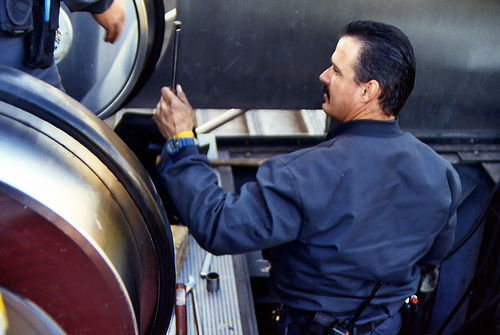
\includegraphics[width=0.775\textwidth]{1989609}
\caption{Immagine di esempio di Flickr30K (id \textit{1989609}) con le seguenti caption di riferimento: 
1) A man wearing blue coveralls is handing a tool to another person;
2) A man in a navy blue jacket holding a tool in his dirty hand;
3) A man in a work uniform passing a tool to another person;
4) Man in a blue jumpsuit attempts to repair an escalator;
5) A man with a mustache works on a broken escalator.
}
\end{figure}

\begin{figure}[ht]
\centering
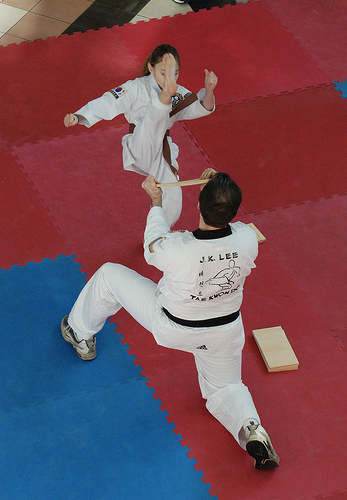
\includegraphics[width=0.5\textwidth]{101362133}
\caption{Immagine di esempio di Flickr30K (id \textit{101362133}) con le seguenti caption di riferimento: 
1) A young female student performing a downward kick to break a board held by her Karate instructor; 
2) Girl about to kick a piece of wood in half while karate instructor holds it; 
3) A girl kicking a stick that a man is holding in tae kwon do class; 
4) A girl in karate uniform breaking a stick with a front kick; 
5) A girl breaking boards by using karate. 
}
\end{figure}

\begin{figure}[H]
\centering
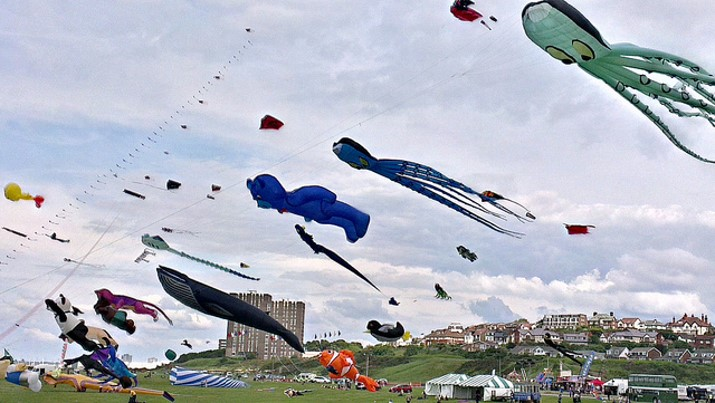
\includegraphics[width=0.8\textwidth]{000000581539}
\caption{Immagine di esempio di \acrshort{coco} (id \textit{000000581539}) con le seguenti caption di riferimento: 
1) Dozens of animal and character shaped floats flying in the air;
2) The sky is full of many colorful flying kites;
3) A bunch of colorful kites flying in the sky;
4) A large number of different kites in the air;
5) A sky filled with kites of every color next to a lush green hillside.
}
\end{figure}


\section{Metriche di valutazione}\label{metriche}
%Le valutazioni umane della traduzione automatica valutano molti aspetti della traduzione, tra cui l'adeguatezza, la fedeltà e la fluidità della traduzione. La maggior parte di questi approcci sono costosi e possono richiedere settimane o mesi per essere completati. 
%Quindi bisogna usare valutazioni automatiche che siano poco costose, veloci, indipendente dalla lingua e altamente correlata alla valutazione umana. Per giudicare la qualità di una traduzione automatica, si misura la sua vicinanza a una o più traduzioni umane di riferimento secondo una metrica numerica.
%Di seguito verranno riportate le metriche di valutazione più utilizzate nello stato dell'arte per valutare i modelli di Image Captioning.

\subsection{BLEU}
\acrshort{bleu} (\acrlong{bleu}) \cite{papineni2002bleu} è una metrica che valuta la qualità della traduzione di un testo e si basa sulla seguente idea: Più una traduzione automatica è vicina a una traduzione umana professionale, meglio è. 
Questa metrica confronta gli n-grammi della frase candidata con gli n-grammi delle traduzioni di riferimento e conta il numero di corrispondenze (le quali sono indipendenti dalla posizione), una traduzione candidata è buona se ne ha tante.
Questo concetto è modellato tramite la precisione che consiste nel conteggio del numero di parole della traduzione candidata che ricorrono in una qualsiasi traduzione di riferimento e il risultato viene diviso per il numero totale di parole nella traduzione candidata.
Sfortunatamente la precisione precedentemente definita non è sufficiente perché si potrebbero avere descrizioni improbabili con punteggi alti, quindi una parola di riferimento deve essere considerata esaurita dopo che è stata identificata una parola candidata corrispondente. L'osservazione precedentemente indicata viene formalizzata tramite la precisione modificata degli n-grammi (Modified n-gram precision), la quale viene calcolata effettuando il conteggio del numero massimo di volte con cui un n-gramma ricorre in ogni singola traduzione di riferimento. Successivamente, si taglia (clip) il conteggio totale di ogni n-gramma per il suo conteggio massimo di riferimento, si sommano i conteggi ottenuti e si divide per il numero totale di n-grammi candidati ottenendo un punteggio $p_n$. La precisione è calcolata separatamente per ogni ordine degli n-grammi, poi le precisioni calcolate sono combinate tramite una media geometrica. Questa misura cattura due aspetti della traduzione: adeguatezza e fluidità. Una traduzione che usa le stesse parole (unigrammi) dei riferimenti tende a soddisfare l'adeguatezza, mentre le corrispondenze di n-grammi più lunghe sono responsabili della fluidità.
La precisione modificata degli n-grammi decade in modo esponenziale con n e \acrshort{bleu} risolve questo problema usando il logaritmo medio con pesi uniformi, che equivale a usare la media geometrica delle precisioni modificate degli n-grammi.
La precisione modificata degli n-grammi penalizza le parole spurie nel candidato che non appaiono in nessuna delle traduzioni di riferimento, quindi il punteggio è penalizzato se una parola ricorre più frequentemente in una traduzione candidata rispetto al suo numero massimo di riferimento. Questo premia l'uso di una parola tutte le volte che è giustificato e penalizza l'uso di una parola più volte di quanto non ricorra in nessuno dei riferimenti. 
Inoltre, questa metrica riesce a penalizzare le traduzioni candidate più lunghe dei loro riferimenti e per gestire le frasi troppo brevi viene utilizzato un fattore moltiplicativo di penalità per la brevità.
Infine, il punteggio \acrshort{bleu} varia da 0 a 1 e per ottenere il valore massimo di 1 la didascalia deve essere identica a una traduzione di riferimento.
\begin{equation*}
BLEU = BP \cdot exp(\sum_{n=1}^N w_n \cdot log(p_n))
\end{equation*}
dove $p_n = \frac{\sum_{C \in \{Candidates\}} \sum_{n-gram \in C} Count_{clip} (n-gram)} {\sum_{C' \in \{Candidates\}} \sum_{n-gram' \in C'} Count_{clip} (n-gram')}$ è la precisione modificata degli n-grammi, Candidates indica le frasi candidate, $w_n = \frac{1}{N}$ sono i pesi uniformi e N indica la tipologia di N-grammi considerati (per esempio, \acrshort{bleu}@4 usa N pari a 4 e considera n-grammi composti da 1 a 4 elementi). Mentre $Count_{clip} = min(Count, MaxRefCount)$ indica il taglio tra il conteggio totale di ogni n-gramma con il suo conteggio massimo di riferimento.
BP è la penalità che regola la brevità e vale 1 se c > r altrimenti $e^{1-r/c}$ se  $c \leq r$, dove c è la lunghezza della didascalia candidata e r è la lunghezza effettiva del corpus di riferimento.
%(insieme delle caption)

\subsection{METEOR}
\acrshort{meteor} (\acrlong{meteor}) \cite{banerjee2005meteor} è una metrica per la valutazione della traduzione che si basa sulla corrispondenza di unigrammi tra la traduzione prodotta dalla macchina e le traduzioni di riferimento prodotte dall'uomo. 
Data una coppia di didascalie da confrontare questa metrica crea un allineamento tra le due stringhe. Quest'ultimo è definito come una mappatura tra gli unigrammi tale che ogni unigramma in ogni stringa corrisponda a zero o a un unigramma nell'altra stringa e a nessun unigramma nella stessa stringa. Così in un dato allineamento, un singolo unigramma in una stringa non può corrispondere a più di un unigramma nell'altra stringa. Questo allineamento è prodotto in modo incrementale attraverso una serie di stadi, i quali prevedono due fasi distinte:
\begin{enumerate}
\item Vengono usati dei moduli esterni diversi che elencano tutte le possibili mappature di unigrammi tra le due stringhe in base a diversi criteri. I moduli utilizzati sono: "exact" mappa due unigrammi se sono esattamente uguali; "porter stem" mappa due unigrammi se sono gli stessi dopo che sono stati stemmatizzati usando lo stemmer Porter; "WN synonymy" mappa due unigrammi se sono sinonimi l'uno dell'altro.
Per impostazione predefinita, il primo stadio utilizza il modulo di mappatura "exact", il secondo il modulo "porter stem" e il terzo il modulo "WN synonymy".
\item Viene selezionato il più grande sottoinsieme delle mappature generate tramite la prima fase, affinché l'insieme risultante costituisca un allineamento dove ogni unigramma corrisponde ad al massimo un unigramma nell'altra stringa. Se più di un sottoinsieme costituisce un allineamento, e ha anche la stessa cardinalità dell'insieme più grande, \acrshort{meteor} seleziona l'insieme che ha il minor numero di incroci di mappature di unigrammi. Formalmente, due mappature di unigrammi ($t_i$, $r_j$) e ($t_k$, $r_l$) (dove $t_i$ e $t_k$ sono unigrammi nella traduzione del sistema mappati rispettivamente agli unigrammi $r_j$ e $r_l$ nella traduzione di riferimento) si dicono incrociate se e solo se la seguente formula valuta un numero negativo:
\begin{equation*}
(pos(t_i) - pos(t_k)) \cdot (pos(r_j)-pos(r_l))
\end{equation*}
dove pos($t_x$) indica la posizione numerica dell'unigramma $t_x$ nella stringa del sistema, mentre pos($r_y$) indica la posizione numerica dell'unigramma $r_y$ nella stringa di riferimento. 
\end{enumerate}
Ogni stadio mappa solo gli unigrammi che non sono stati mappati a nessun unigramma in nessuna delle fasi precedenti. Quindi l'ordine in cui gli stadi vengono eseguiti impone diverse priorità sui moduli di mappatura impiegati dai diversi stadi. La metrica \acrshort{meteor} mappa prima due unigrammi in base alla loro forma superficiale, ed esegue lo stemming solo se le forme superficiali non corrispondono (o se la mappatura basata sulle forme superficiali risulta troppo "costosa" in termini di numero totale di incroci). Per impostazione predefinita, il primo stadio utilizza il modulo di mappatura "esatto", il secondo il modulo "porter stem" e il terzo il modulo "WN synonymy".
Una volta che tutti gli stadi sono terminati ed è stato generato un allineamento finale tra la didascalia del sistema e la didascalia di riferimento, il punteggio \acrshort{meteor} per questa coppia di traduzioni è calcolato così:
\begin{equation*}
METEOR = Fmean \cdot (1 - Penalty)
\end{equation*}
Dove $Fmean = \frac{10\cdot PR}{R+9\cdot P}$ è la media armonica tra la precision P e la recall R, viene assegnata più importanza alla recall.
$P = \frac{m}{w_t}$ è calcolata come il rapporto tra il numero di unigrammi nella traduzione del sistema che sono mappati (m) e il numero totale di unigrammi nella traduzione del sistema ($w_t$). Mentre $R = \frac{m}{w_r}$ è calcolato come il rapporto tra il numero di unigrammi nella traduzione del sistema che sono mappati (m) e il numero totale di unigrammi nella traduzione di riferimento ($w_r$).
Infine, $Penalty = 0.5 \cdot (\frac{\#chuncks}{\#unigrams\_matched})^3$ è una penalità che gestisce le corrispondenze lunghe, la quale considera tutti gli unigrammi nella traduzione del sistema che sono mappati a unigrammi nella traduzione di riferimento. Gli unigrammi mappati sono raggruppati nel minor numero possibile di chunks affinché essi siano in posizioni adiacenti nella traduzione del sistema, e siano anche mappati a unigrammi che sono in posizioni adiacenti nella traduzione di riferimento. 


Riassumendo questa metrica abbina gli unigrammi in base alle loro forme superficiali, alle forme stemmate e ai significati. Quindi, l'abbinamento implementato supporta non solo la corrispondenza tra parole che sono identiche nelle due stringhe confrontate, ma può anche abbinare parole che sono semplici varianti morfologiche l'una dell'altra (cioè che hanno la stessa radice), e parole che sono sinonimi l'una dell'altra. Una volta trovate tutte le corrispondenze generalizzate di unigrammi tra le due stringhe, viene usata la metrica \acrshort{meteor} per assegnare un punteggio a questa corrispondenza sfruttando una combinazione di unigram-precision, unigram-recall e una misura di frammentazione. Quest'ultima è progettata per catturare direttamente quanto le parole abbinate nella traduzione automatica siano ben ordinate in relazione al riferimento.
Se è disponibile più di una caption di riferimento, la didascalia predetta viene valutata rispetto a ciascun riferimento in modo indipendente e viene riportato il punteggio migliore.
Il valore della metrica varia tra -1,0 (correlazione completamente negativa) e +1,0 (correlazione completamente positiva). 

\subsection{CIDEr}\label{cider}
\acrshort{cider} (\acrlong{cider}) \cite{vedantam2015cider} è una metrica nata appositamente per la valutazione delle performance dei modelli di Image Captioning, misura la somiglianza di una frase generata con un insieme di frasi di verità scritte da esseri umani ed è fortemente correlata al giudizio umano. La somiglianza delle frasi permette di catturare implicitamente le nozioni di grammaticalità, salienza, importanza e accuratezza (precision e recall).
Data una frase candidata e un insieme di descrizioni di immagini Si = {$si_1$, . . . , $si_m$} di riferimento. Tutte le parole nelle frasi (sia quelle candidate che quelle di riferimento) vengono mappate alle loro forme radici e ogni frase viene rappresentata dall'insieme di n-grammi presenti in essa.
Successivamente viene usata la tecnica \acrfull{tfidf} per effettuare una rappresentazione vettoriale di ogni n-gramma $w_k$. Questa tecnica codifica quanto spesso gli n-grammi nella frase candidata sono presenti nelle frasi di riferimento, quanto gli n-grammi non presenti nelle frasi di riferimento non dovrebbero essere presenti nella frase candidata e quanto gli n-grammi che ricorrono comunemente in tutte le frasi del set di dati dovrebbe avere un peso inferiore, poiché probabilmente sono meno informativi. 
Il numero di volte che un n-gramma $w_k$ ricorre in una frase di riferimento $s_{ij}$ è indicato con $h_k(s_{ij})$ o $h_k(c_i)$ per la frase candidata $c_i$.
La rappresentazione \acrshort{tfidf} $g_k(s_{ij})$ per ogni n-gramma $w_k$ della frase $s_{ij}$ è calcolato tramite:
\begin{equation*}
g_k(s_{ij}) = \frac{h_k(s_{ij})}{\sum_{w_l\in \Omega} h_l(s_{ij})} \cdot log(\frac{|I|}{\sum_{I_p \in I} min(1, \sum_q h_k (s_{pq}))})
\end{equation*}
dove $\Omega$ è il vocabolario di tutti gli n-grammi e I è l'insieme delle immagini.
Infine, il punteggio \acrshort{cider}$_n$ per n-grammi di lunghezza n è calcolato usando la media della similarità del coseno tra la frase candidata e le frasi di riferimento, la formula è la seguente:
\begin{equation*}
CIDEr_n(c_i, S_i) = \frac{1}{m} \sum_j \frac{g_n(c_i) \cdot g_n(s_{ij})} {||g_n(c_i)|| \cdot ||g_n(s_{ij}) ||}
\end{equation*}
dove $g_n(c_i)$ è il vettore che contiene la rappresentazione \acrshort{tfidf} di $c_i$, mentre $g_n(s_{ij})$ contiene quella di $s_{ij}$.
Vengono usati n-grammi più lunghi per catturare proprietà grammaticali e una semantica più ricca (empiricamente il valore migliore è N=4), i quali sono combinati tramite:
\begin{equation*}
CIDEr(c_i, S_i) = \sum^N_{n=1} \frac{1}{N} \cdot CIDEr_n(c_i, S_i)
\end{equation*}
\subsection{SPICE}
\acrshort{spice} (\acrlong{spice}) \cite{anderson2016spice} è una metrica nata per la valutazione delle performance dei modelli di Image Captioning e misura la qualità delle didascalie generate analizzando il loro contenuto semantico.
%Questa metrica risolve i limiti delle metriche di valutazione automatica basate sugli n-grammi, la sovrapposizione di n-grammi non è né necessaria né sufficiente perché due frasi trasmettano lo stesso significato.
Le didascalie candidate C e quelle di riferimento S vengono trasformate in una rappresentazione semantica basata sugli scene graph. Questa tipologia di grafo codifica esplicitamente gli oggetti, gli attributi e le relazioni che si trovano nelle didascalie delle immagini, astraendo la maggior parte delle idiosincrasie lessicali e sintattiche del linguaggio naturale nel processo.
Viene costruito un grafo per la didascalia candidata, indicato con G(C), e un grafo per le didascalie di riferimento S, indicato con G(S); quest'ultimo è ottenuto come l'unione dei grafi di scena G($s_i$) $\forall(s_i \in S)$ combinando i nodi di oggetti sinonimi.
\begin{equation*}
G(C) = (O(C), E(C), K(C))
\end{equation*}
I grafi hanno come nodi O($\cdot$) gli oggetti menzionati nella didascalia e come archi E($\cdot$) le relazioni tra gli oggetti, inoltre i nodi prevedono degli attributi K($\cdot$).
La costruzione del grafo prevede due fasi:
\begin{enumerate}
\item Estrazione di alberi di dipendenza tramite lo Stanford Scene Graph Parser, il quale identifica le dipendenze sintattiche tra le parole delle didascalie;
\item Conversione degli alberi di dipendenza in scene graph utilizzando un sistema a regole;
\end{enumerate}
Per valutare la somiglianza dei grafi candidati e di riferimento, le relazioni semantiche nel grafo sono trattate come una congiunzione di proposizioni logiche, o tuple. La seguente funzione T restituisce tuple logiche da uno scene graph:
\begin{equation*}
T(G(C))  \stackrel{\Delta}{=} O(C) \cup E(C) \cup K(C)
\end{equation*}
Ogni tupla contiene da uno a tre elementi, i quali rappresentano rispettivamente oggetti, attributi e relazioni.
La metrica \acrshort{spice} assume un valore tra 0 e 1, la formula è la seguente:
\begin{equation*}
SPICE(C,S) = F_1(C,S) = \frac{2 \cdot P(C,S) \cdot R(C,S)}{P(C,S) + R(C,S)}
\end{equation*}
Dove $P(C,S) = \frac{|T(G(C)) \bigotimes T(G(S))|}{|T(G(C))|}$ è la precision, mentre $R(C,S) = \frac{|T(G(C)) \bigotimes T(G(S))|}{|T(G(S))|}$ è la recall e $\bigotimes$ è l'operatore di corrispondenza binaria che restituisce le tuple corrispondenti tra due scene graph (le tuple sono considerate corrispondenti se la loro forma radice è uguale).
\acrshort{spice} misura quanto bene i generatori di didascalie recuperano gli oggetti, gli attributi e le relazioni tra loro; presuppone implicitamente che le didascalie siano ben formate.

\chapter{Approccio}
Recentemente sono stati sviluppati modelli linguistici pre-addestrati su molti task composti da una componente visiva e da una linguistica (come Image Captioning, Visual Question Answering, Image-text Retrieval, etc), i quali prevedono coppie immagine-testo. L'obiettivo del pre-addestramento è quello di imparare rappresentazioni cross-modali di coppie immagine-testo in modo self-supervised affinché il modello possa essere adattato per servire vari compiti tramite fine-tuning sul task specifico. Questo è motivato da alcuni studi recenti \cite{zhou2020unified, li2019visualbert, li2020unicoder}, i quali hanno dimostrato che il pre-training di modelli su ampi dataset composti da coppie immagine-testo è molto utile per imparare efficacemente rappresentazioni generiche (cross-modali) e il fine-tuning su task specifici raggiunge risultati allo stato dell'arte.

In questo lavoro è stato sfruttato il modello linguistico pre-addestrato creato da Li et all. \cite{li2020oscar, zhang2021vinvl} chiamato \acrshort{oscar}$_+$, il quale è una variante di \acrshort{bert} e richiede come visual encoder un modello in grado di estrarre regioni visuali da un'immagine. %In questa tesi è stato scelto questo modello poiché è molto interessante e quando è iniziato questo progetto era quello con le performance più elevante sul benchmark di Image Captioning di \acrshort{coco}.

\acrshort{oscar}$_+$ si basa sull'assunzione che gli esseri umani percepiscono il mondo attraverso molti canali. Anche se ogni singolo canale potrebbe essere incompleto o rumoroso, i fattori importanti sono ancora percepibili poiché tendono a essere condivisi tra più canali (ad esempio, un oggetto può essere descritto visivamente e verbalmente). 
Infatti, questo modello è in grado di imparare rappresentazioni che catturano fattori invarianti per canale (o per modalità) a livello semantico.

Ogni coppia immagine-testo di input viene rappresentata come una tripla \textbf{Word-Tag-Image} (w, q, v), dove w è la sequenza di word embedding del testo, q è la sequenza di word embedding dei tag oggetto rilevati dall'immagine e v è l'insieme dei vettori regione dell'immagine. I tag q sono utilizzati come punti di collegamento che facilitano l'apprendimento dell'allineamento semantico immagine-testo. Questo è ulteriormente motivato dall'osservazione che nei dati di addestramento, gli oggetti importanti in un'immagine sono spesso presenti anche nel testo abbinato all'immagine. Per esempio, nel dataset \acrshort{coco} \cite{lin2014microsoft} le percentuali che un'immagine e il suo testo abbinato condividano almeno 1, 2, 3 oggetti sono rispettivamente 49.7\%, 22.2\%, 12.9\%. Inoltre, molto spesso quando sono usate parole diverse dai tag dell'oggetto vengono comunque utilizzate parole semanticamente simili o correlate, gli allineamenti tra q e w sono relativamente facili da identificare utilizzando il modello pre-addestrato \acrshort{bert} \cite{devlin2018bert}.


\section{Visual Encoder}\label{visual_encoder}
La rappresentazione del contenuto visivo v e il rilevamento dei tag oggetto q delle regioni per la tripla (w, q, v) sono stati effettuati tramite tre modalità differenti: la prima prevede un modello di Object Detection (lo stesso utilizzato dagli autori del paper \cite{zhang2021vinvl} da cui è partito questo lavoro di tesi); la seconda prevede un approccio innovativo che utilizza un ensemble composto da un modello di Panoptic Segmentation e da un modello di Instance Segmentation; la terza si basa sull'unione delle due modalità precedenti.

\subsection{Object Detection}\label{object_detection}

Data un'immagine con K regioni di oggetti, viene utilizzato un modello di Object Detection per estrarre la semantica visiva di ogni regione come (v', z), dove v' $\in R^P$ è un vettore P-dimensionale (P = 2048) estratto dall'input dell'ultimo linear classification layer della detection head del modello di Object Detection e z è un vettore R-dimensionale rappresentante la posizione della regione (R = 6 che sono le coordinate del punto in alto a sinistra, in basso a destra, l'altezza e lunghezza della bounding box). Successivamente v' e z sono concatenati per formare un vettore di feature della regione sensibile alla posizione, che viene ulteriormente trasformato in v utilizzando una proiezione lineare per garantire che abbia la stessa dimensione vettoriale di quella degli embedding delle parole.
Lo stesso modello viene utilizzato per rilevare un insieme di tag ad alta precisione, i quali sono le classi degli oggetti rilevati all'interno dell'immagine, e q è la sequenza di embedding delle parole dei tag.
Il modello di Object Detection utilizzato si basa sull'architettura \textbf{\acrshort{faster_rcnn}}\footnote{\url{https://github.com/microsoft/scene_graph_benchmark}} \cite{ren2015faster}, il quale è stato pre-addestrato sui dataset: \acrshort{coco} \cite{lin2014microsoft}, OpenImagesV5 \cite{kuznetsova2020open}, Objects365V1 \cite{shao2019objects365} e Visual Genome\footnote{Visual Genome è un dataset composto da 108K immagini densamente annotate con scene graph contenenti oggetti, attributi e relazioni} \cite{krishna2017visual}. Questi dataset hanno caratteristiche complementari e sono estremamente sbilanciati in termini di dimensioni, vocabolario degli oggetti e numero di annotazioni per ogni classe. Quindi viene creato un corpus unificato che combina i vari dataset: rimuovendo le classi di coda con poche istanze, bilanciando il contributo di ogni dataset (vengono utilizzate 8 copie di \acrshort{coco}, 8 copie di Visual Genome, 2 copie di Objects365 e una copia di OpenImages ottenendo in totale 5.43M di immagini), effettuando data augmentation (flipping orizzontale e addestramento multi-scala) e unificando i vocabolari degli oggetti.
Infine, al modello di Object Detection precedentemente creato viene aggiunto un ramo per la predizione degli attributi e l'architettura risultante viene utilizzata per effettuare fine-tuning sul dataset Visual Genome.
Il modello finale riesce a prevedere fino a 1594 classi di oggetti e 524 attributi visivi.
La componente che si occupa della predizione degli attributi è stata aggiunta poiché permette di ottenere rappresentazioni delle regioni più significative \cite{anderson2018bottom}.

\subsection{Image Segmentation}\label{image_segmentation}
Nonostante il modello di Object Detection sia stato appositamente sviluppato per questa tipologia di task esistono diverse regioni, rappresentanti oggetti di classi diverse, codificate tramite feature molto simili. 
Infatti, le regioni estratte sono risultate spesso sovrapposte, rumorose e ambigue, questo inevitabilmente risulta in feature delle regioni meno significative.
Per esempio, nella Figura \ref{figura:risultato_detection} le regioni evidenziate non sono facilmente distinguibili poiché si sovrappongono pesantemente. Infatti, la regione che rappresenta l'oggetto di classe Door e la regione che rappresenta l'oggetto di classe Boy hanno delle region feature con cosine similarity\footnote{La cosine similarity misura la somiglianza tra due vettori calcolando l'angolo del coseno tra di loro. Il valore di similitudine è compreso tra -1 e +1, dove -1 indica una corrispondenza esatta ma opposta e +1 indica due vettori uguali.} pari a 0.8, però rappresentano due oggetti totalmente diversi.
\begin{figure}[ht]
\centering
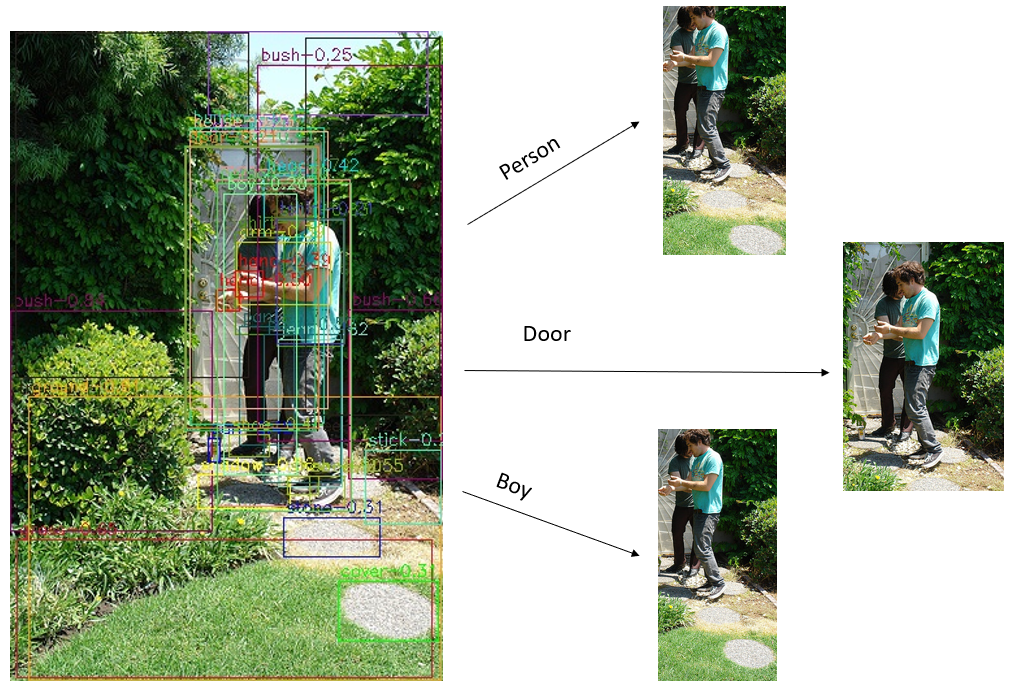
\includegraphics[width=0.8\textwidth]{risultato_detection}
\caption{Risultato del modello di Object Detection su un'immagine in cui vengono evidenziate alcune regioni sovrapposte, rumorose e ambigue che rappresentano istanze diverse (Flickr30K id 1000092795).}\label{figura:risultato_detection}
\end{figure}
Per risolvere il problema è stata utilizzata la segmentazione, la quale oltre alla classe e alla bounding box permette di determinare una maschera di segmentazione che permette di estrarre solamente l'istanza di interesse rimuovendo i pixel superflui.


In questo lavoro di tesi le risorse computazionali sono state limitate e per ottenere i risultati migliori possibili sono stati utilizzati due modelli di segmentazione già addestrati con ottime performance.
Nel dettaglio si tratta di un modello di Panoptic Segmentation allenato su \acrshort{coco} Panoptic \cite{lin2014microsoft} (composto da \acrshort{coco} instances e \acrshort{coco} stuff), il quale permette di ottenere segmentazioni delle immagini coerenti, ricche e complete.
Questo modello è in grado di predire solamente 133 classi e per aumentare il numero di oggetti riconoscibili è stato utilizzato un modello aggiuntivo di Instance Segmentation allenato su \acrshort{lvis} \cite{gupta2019lvis} (\acrlong{lvis}).
Quest'ultimo dataset è molto interessante poiché prevede 1203 categorie di oggetti ed è facilmente integrabile con \acrshort{coco}, infatti \acrshort{lvis} è un'estensione di \acrshort{coco} instances e prevede per le immagini maschere di segmentazione di qualità superiore che seguono meglio i confini degli oggetti.
Il modello di Panoptic Segmentation utilizzato è \textbf{\acrshort{detr}} \cite{carion2020end}, mentre il modello di Instance Segmentation utilizzato è una \acrshort{mask_rcnn} \cite{gupta2019lvis, he2017mask} (identificata con \textbf{Mask-\acrshort{lvis}}) allenata su \acrshort{lvis} tramite tecniche di data augmentation, poiché il dataset presenta categorie molto sbilanciate.
I due modelli insieme riescono a riconoscere 1280 classi, le quali sono state unificate gestendo eventuali sinonimi (per esempio: tv e television), le classi troppo rare e specifiche sono state raggruppate nella classe più generica (per esempio Bible è stata inserita in book),  è stata rimossa la classe più generica dai tag di classe che la contengono (per esempio dalla classe "beef (food)" è stato rimosso (food), diventando solo "beef") e le classi finali ottenute sono 1248.



Data un'immagine vengono utilizzati Mask-\acrshort{lvis} e \acrshort{detr} per estrarre le bounding box, le maschere di segmentazione e le classi degli oggetti. L'estrazione delle componenti q e v della tripla (vedere Sezione \ref{object_detection} per maggiori dettagli), per ogni istanza rilevata, è effettuata tramite le seguenti fasi:
\begin{enumerate}
\item Viene estratto l'oggetto dall'immagine di partenza utilizzando la maschera predetta e sul risultato viene utilizzata la bounding box per estrarre solo la regione di interesse. Dall'immagine originale viene rimossa l'istanza rilevata utilizzando la maschera di segmentazione affinché le prossime estrazioni non la contengano.
Inoltre, se nelle estrazioni successive la regione estratta ha più del 60\% di pixel bianchi viene presa l'immagine di partenza senza rimozioni per effettuare l'estrazione dell'oggetto segmentato, in questo modo si ottiene un buon contenuto visivo dell'oggetto riducendo le sovrapposizioni. Quindi in questa fase si ottiene una regione contenente l'oggetto segmentato con sfondo bianco;
\item La regione ottenuta precedentemente viene ridimensionata utilizzando l'interpolazione bilineare\footnote{L'interpolazione bilineare, durante il ridimensionamento e l'interpolazione di nuovi pixel, utilizza i pixel adiacenti 2x2 dell'immagine per calcolare la media ponderata utilizzata per ottenere il pixel interpolato.} \cite{jaderberg2015spatial} (questa tipologia di interpolazione è stata usata anche nel modello \acrshort{mask_rcnn} per ottenere risultati migliori, vedere sezione \ref{mask_section} per maggiori dettagli), la quale si comporta molto bene sia nei casi di riduzione (downscale) sia in quelli di aumento della dimensione (upscale) della regione. Questa fase è molto importante per la determinazione delle feature dell'oggetto;
\item Vengono estratte le feature v' della regione ridimensionata tramite il modello \acrshort{resnet} \cite{he2016deep}, quest'ultimo è stato utilizzato per unificare le rappresentazioni e perché il modello di Object Detection utilizzato usa \acrshort{resnet} come backbone. Le feature v' vengono concatenate insieme al vettore z contenente la posizione dell'oggetto. Infine, v' e z vengono concatenati per ottenere il vettore di feature della regione finale (vedere Sezione \ref{object_detection} per maggiori dettagli);
\item Viene utilizzata la label di classe predetta per ottenere il word embedding q;
\end{enumerate}
Infine, una volta che sono stati estratti tutti gli oggetti l'immagine finale pulita dalle segmentazioni viene valutata verificando se il numero di pixel non bianchi che contiene siano maggiori del 40\% rispetto ai pixel totali. Se questa condizione è rispettata allora l'immagine contenente i pixel che non sono stati segmentati viene trattata come una regione assegnandogli la classe Other e come bounding box il vettore \texttt{[0, 0, image\_width, image\_height]} (questo approccio ha preso ispirazione dal dataset \acrshort{coco} stuff, nel quale i pixel non segmentati vengono considerati nella classe Other).


La Figura \ref{figura:pipeline_segmentation} mostra l'estrazione delle feature per le istanze rilevate tramite segmentazione. Le fasi utilizzate vengono ripetute prima per tutti gli oggetti rilevati tramite il modello Mask-\acrshort{lvis} e successivamente per tutti gli oggetti rilevati tramite \acrshort{detr}, vengono effettuati in questo ordine perché la Panoptic Segmentation può rilevare classi meno specifiche e questo può portare a sovrapposizioni.
\newpage
\begin{figure}[h]
\centering
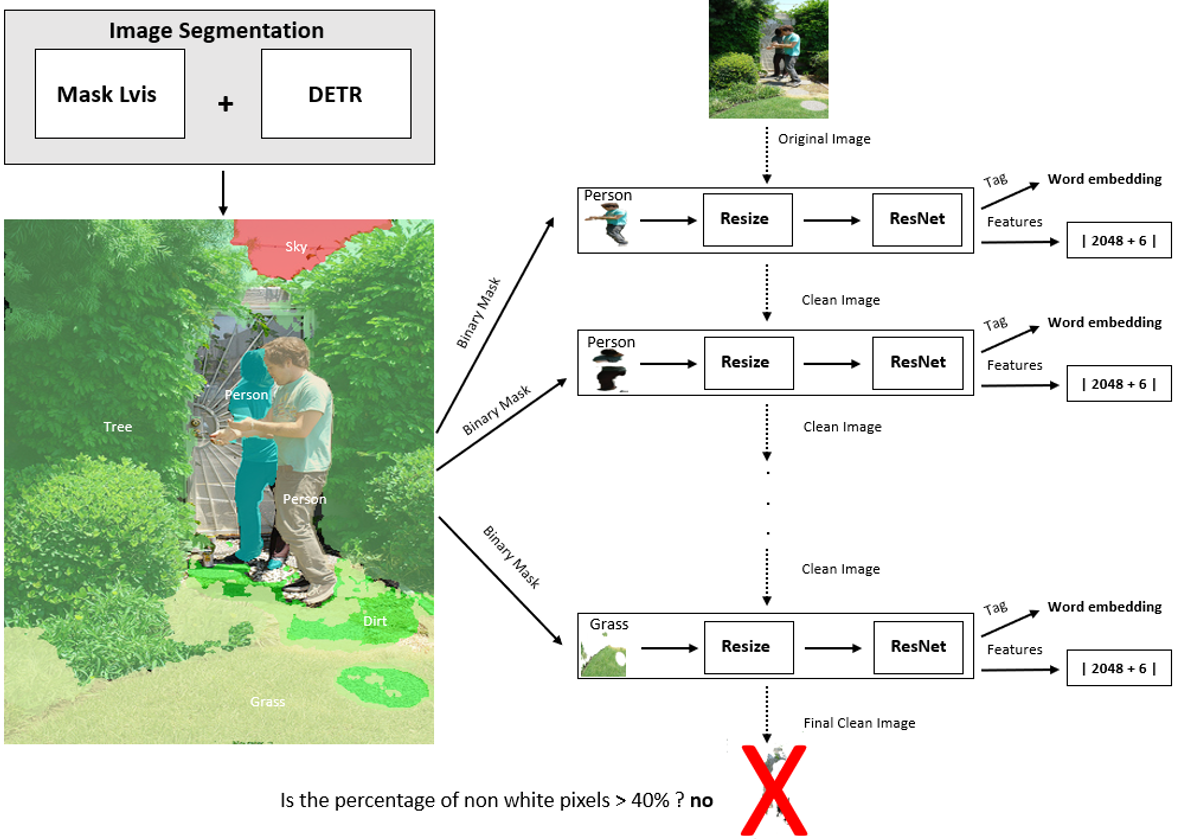
\includegraphics[width=0.95\textwidth]{pipeline_segmentation}
\caption{Illustrazione riassuntiva dell'estrazione delle feature dagli oggetti ottenuti tramite Image Segmentation.}\label{figura:pipeline_segmentation}
\end{figure}

\subsection{Combinazione tra Object Detection e Image Segmentation}\label{combinazione}
L'ensemble dei modelli di segmentazione riesce a predire meno classi rispetto al modello di Object Detection utilizzato e spesso oggetti molto importanti che sono imprescindibili per la comprensione del contenuto visivo e per la generazione della caption non vengono rilevati. La Figura \ref{figura:segmentazione_regioni_mancanti} mostra un caso in cui viene rilevata una sola regione raffigurante una persona ma all'interno dell'immagine sono presenti altri oggetti molto importanti, come la chitarra, che non vengono rilevati tramite segmentazione. 
\begin{figure}[ht!]
\centering
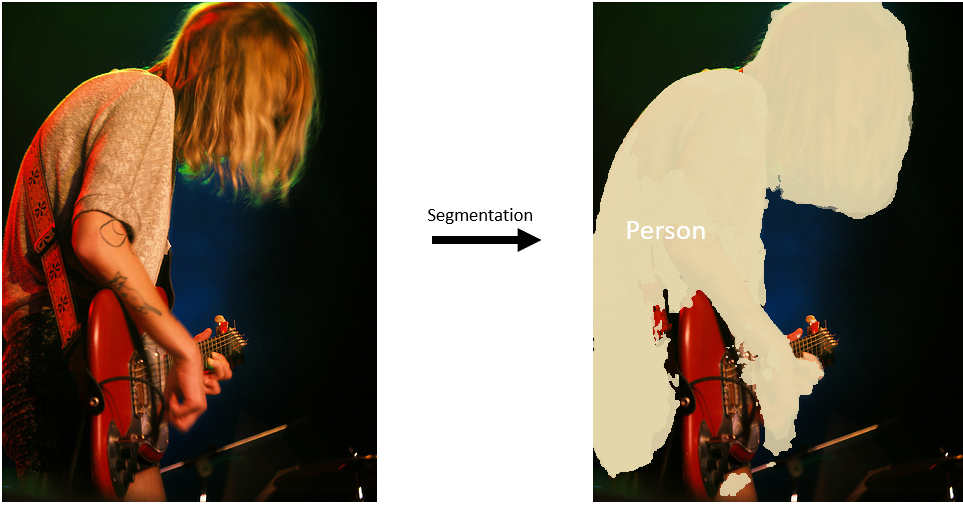
\includegraphics[width=0.9\textwidth]{segmentazione_regioni_mancanti.png}
\caption{Illustrazione in cui si può notare la mancanza della rilevazione di oggetti importanti per comprendere il contenuto visivo dell'immagine e per generare una caption di buona qualità. Id immagine Flickr30K: 6184270681}\label{figura:segmentazione_regioni_mancanti}
\end{figure}
La segmentazione in media riesce a estrarre 14 oggetti con un numero massimo di istanze rilevate in una singola immagine pari a 71 e con un minimo di 1. Mentre, il modello di Object Detection rileva in media 44 oggetti con un numero massimo di istanze rilevate in una singola immagine pari a 100 e con un minimo di 10.
Inoltre, l'ensemble dei modelli di segmentazione a volte ha difficoltà nella predizione delle classi corrette.



Il primo problema precedentemente individuato è stato risolto includendo le regioni predette tramite Object Detection non rilevate tramite segmentazione. Una regione estratta dal modello di Object Detection risulta non rilevata se il suo vettore rappresentante la bounding box non ha cosine similarity maggiore di 0.98 con il vettore della bounding box di nessun oggetto estratto tramite l'ensemble di Image Segmentation.


Mentre, il secondo problema è stato risolto tramite una pipeline di correzione delle classi estratte tramite segmentazione, dove vengono recuperate le regioni simili estratte tramite Object Detection.
La \textit{pipeline di correzione delle classi} prevede le seguenti fasi:
\begin{enumerate}
    \item Per ogni oggetto rilevato tramite Image Segmentation viene creato un insieme di regioni simili rilevate tramite Object Detection utilizzando la cosine similarity applicata sui vettori rappresentanti la bounding box e un valore di similitudine minimo utilizzato per filtrare. Dall'insieme creato vengono estratti i tre oggetti più simili basandosi sulle tre modalità seguenti:
    \begin{enumerate}[leftmargin=2.5cm,label=Metodo \arabic*:]
        \item recupera l'oggetto considerando l'etichetta di classe più frequente e tra questi prende quello con la confidenza di predizione più elevata;
        \item prende l'oggetto con la bounding box che ottiene il punteggio di cosine similarity maggiore;
        \item prende l'oggetto il cui vettore delle feature ottiene il valore di cosine similarity più alto considerando il vettore delle feature dell'oggetto segmentato che si sta valutando;
    \end{enumerate}
    In tutti i metodi se ci sono più oggetti candidati che sopravvivono, tra questi viene preso quello con la confidenza di predizione maggiore.
    Quindi questa fase termina restituendo un insieme composto da tre oggetti (uno per ogni metodo);
    \item Su ogni oggetto rilevato come candidato viene calcolato uno score pesato che considera la similarità tra le feature, la similarità tra i word embedding e la confidenza di predizione della classe rilevata tramite Object Detection. La formula \ref{score} viene utilizzata per calcolare il punteggio che viene assegnato a ogni oggetto.
\end{enumerate}
\begin{equation}\label{score}
        score = features\_similarity  \cdot  0.6 + words\_similarity  \cdot  0.3 + conf  \cdot  0.1
\end{equation}
Infine, viene presa la classe dell'oggetto che ottiene lo score più alto, la quale andrà a sostituire la classe dell'oggetto estratto tramite segmentazione che si sta valutando.
Nello score è stata privilegiata la similarità tra i vettori delle feature.


\section{Language Model}
Il modello linguistico utilizzato si basa su \acrshort{bert} \cite{devlin2018bert} e si chiama \textbf{\acrshort{oscar}$_+$} \footnote{\url{https://github.com/microsoft/Oscar}}, questo modello è stato pre-addestrato su un grande dataset D composto dai dataset vision-language esistenti, tra cui quelli di Image Captioning: \acrshort{coco} \cite{lin2014microsoft}, Conceptual Captions (CC) \cite{sharma2018conceptual}, SBU captions \cite{ordonez2011im2text}, Flickr30k \cite{young2014image}; i dataset di Visual Question Answering: GQA \cite{hudson2019gqa}, VQA \cite{goyal2017making}, VG-QA; infine, viene utilizzata una porzione del dataset OpenImages di Image Tagging. In totale, il dataset finale è composto da 5.65 milioni di immagini uniche e da 8.85 milioni di triple testo-tag-immagine, le quali sono state estratte tramite il modello di Object Detection.
Il pre-training di \acrshort{oscar}$_+$ è stato effettuato utilizzando la funzione obiettivo riportata nell'equazione \ref{funzione_obiettivo} composta dalla combinazione di due loss function diverse.

\begin{equation}\label{funzione_obiettivo}
L_{Pre-training} = L_{MTL} + L_{CL3}
\end{equation}

La funzione obiettivo definita precedentemente è calcolata considerando l'input del modello come una composizione di due prospettive diverse:
\begin{equation*}
x \stackrel{\Delta}{=} [\textcolor{red}{w}, \textcolor{green}{q}, \textcolor{green}{v}] = [\textcolor{red}{w}, \textcolor{red}{q} , \textcolor{green}{v}] \stackrel{\Delta}{=} x'
\end{equation*}
dove il rosso indica la rappresentazione del linguaggio e il verde la rappresentazione dell'immagine.
Inoltre, x indica la \textit{modality view} usata per distinguere le rappresentazioni tra un testo e un'immagine; mentre $x'$ è la \textit{dictionary view} usata per distinguere i due diversi spazi semantici in cui l'input è rappresentato.


La dictionary view usa la \textbf{\acrfull{mtl}}, in questa modalità i token dei tag degli oggetti (o answer per i dati di visual question answering) e i token delle parole delle caption (o question per i dati di visual question answering) condividono lo stesso spazio semantico linguistico, mentre le feature delle regioni dell'immagine si trovano nello spazio semantico visivo. La \acrlong{mtl} per il pre-training è applicata sulla sequenza discreta di token, la quale è definita come $h \stackrel{\Delta}{=} [w, q]$. A ogni iterazione, viene mascherato casualmente ogni token di input in h con una probabilità del 15\% e il token $h_i$ viene sostituito con un token speciale \texttt {[MASK]}. L'obiettivo dell'addestramento è prevedere questi token mascherati basandosi sui token circostanti $h_{\setminus i}$ e su tutte le feature dell'immagine v, minimizzando la log-likelihood negativa:
\begin{equation*}
L_{MTL} = -E_{(v, h) \sim D} \hspace{0.1cm} log \hspace{0.1cm} p(h_i|h_{\setminus i},v)
\end{equation*}
Questa funzione di perdita è simile a quella usata da \acrshort{bert}, in questa variante la parola o l'etichetta mascherata deve essere recuperata da ciò che la circonda, con la partecipazione delle informazioni aggiuntive dell'immagine che aiutano a definire i word embedding appresi nel contesto della visione.


La modality view usa la \textbf{\acrfull{lcl3}}, nella quale vengono definite due tipologie di triple inquinate (non abbinate) per i due tipi di campioni di allenamento. Le triple inquinate sono composte da ($w'$, q, v) = \{caption, image-tags, image-features\} per i dati di image captioning e image tagging, e (w, $q'$, v) = \{question, answer, image-features\} per i dati di visual question answering (il carattere con $'$ indica la componente inquinata). Successivamente viene usato un fully-connected (FC) layer f($\cdot$) in cima a esso come un classificatore con 3 possibili valori, il quale prevede: se la tripla è abbinata (c = 0), contiene una w inquinata (c = 1) o contiene una q inquinata (c = 2).
Quindi, il modello è addestrato a distinguere triple vere o false e questa funzione di perdita è definita come:
\begin{equation*}
L_{CL3} = -E_{(w, q, v; c) \sim \widetilde{D}} \hspace{0.1cm} log \hspace{0.1cm} p(c|f(w, q, v))
\end{equation*}
dove il dataset (w, q, v; c) $\in \widetilde{D}$ contiene il 50\% di triple corrette, il 25\% di triple con w inquinata e il 25\% di triple con q inquinata. 
Le triple inquinate prevedono la sostituzione di q con una probabilità del 50\% con una sequenza di tag o answer diversa campionata casualmente dal dataset; mentre, per w inquinata la sostituzione avviene sulle caption e question.


La funzione di perdita definita consente di ottenere delle performance superiori quando viene effettuato il fine-tuning sul task specifico.

\begin{figure}[ht]
\centering
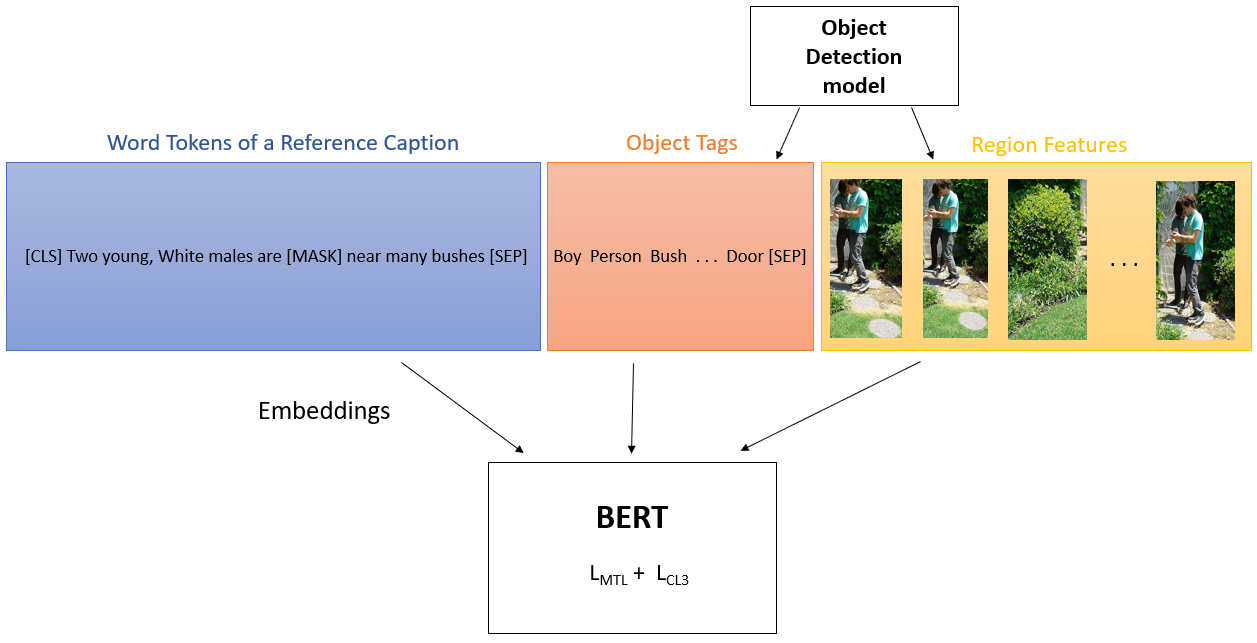
\includegraphics[width=0.99\textwidth]{architettura}
\caption{Illustrazione riassuntiva del pre-training del modello \acrshort{oscar}$_+$, il fine-tuning sul task di Image Captioning prevede come loss solo la \acrshort{mtl} e le componenti q e v della tripla possono essere estratte utilizzando il modello di Object Detection, l'ensemble dei modelli di segmentazione o la combinazione tra detection e segmentation.}
\end{figure}

\subsection{Fine-Tuning}

Il modello \acrshort{oscar}$_+$ pre-addestrato viene utilizzato per l'Image Captioning effettuando fine-tuning mantenendo lo stesso input composto da triple, ma la funzione di perdita è composta solamente dalla \acrlong{mtl}. Le componenti q e v della tripla possono essere estratte tramite il modello di Object Detection, tramite l'ensemble dei modelli di segmentazione o tramite la combinazione tra Object Detection e Image Segmentation. La self-attention mask di \acrshort{bert} viene vincolata affinché un token della didascalia possa partecipare solo ai token prima della sua posizione per simulare un processo di generazione unidirezionale.

 
%Recentemente è stato dimostrato \cite{rennie2017self} che il training basato su metriche non differenziabili genera bias durante l'inferenza e non consente di ottimizzare il modello direttamente sulle metriche per il compito da svolgere. Quindi sono state sviluppate tecniche che risolvono questi problemi e le metodologie in questione si basano su approcci di reinforcement learning.
Oltre al fine-tuning precedente per migliorare l'apprendimento a livello di sequenza viene effettuato un ulteriore fine-tuning del modello ottenuto applicando un approccio di ottimizzazione basato sul \acrlong{rl} chiamato \acrfull{scst} \cite{rennie2017self}, vedere Sezione \ref{scst} per maggiori dettagli. Esistono diversi modelli \cite{anderson2018bottom, zhou2020unified, li2020oscar, zhang2021vinvl} che hanno utilizzato questo approccio ottenendo miglioramenti significativi in fase di test. In questo approccio il modello di Image Captioning è considerato come un agente i cui parametri determinano una politica.
A ogni passo temporale, l'agente esegue la politica per scegliere un'azione, cioè la previsione della prossima parola nella frase generata. Una volta raggiunta la fine della sequenza l'agente riceve una ricompensa e lo scopo dell'addestramento è di ottimizzare i parametri dell'agente per massimizzare la ricompensa prevista.
La ricompensa viene determinata utilizzando la metrica \acrshort{cider} (vedere Sezione \ref{cider} per maggiori dettagli), la quale si correla bene con il giudizio umano ed è stata pensata appositamente per il task di Image Captioning.
% Tramite questa tecnica la ricompensa è normalizzata rispetto a un valore di base per ridurre la varianza.  ??????
L'approccio di \acrlong{rl} non viene applicato fin da subito perché risulta difficile per questa procedura ottenere miglioramenti significativi in un tempo accettabile (per esempio con le risorse a nostra disposizione una singola epoca con \acrshort{scst} richiede circa undici ore), quindi viene effettuato prima un altro fine-tuning usando tecniche standard e poi viene utilizzato \acrshort{scst}.
\subsection{Inferenza}
Durante l'inferenza, prima vengono rilevate e codificate le regioni dell'immagine e i tag degli oggetti rilevati tramite una delle modalità specificate nella Sezione \ref{visual_encoder}. Successivamente il modello \acrshort{oscar}$_+$ utilizza le feature estratte per effettuare la generazione della caption, la quale inizia inserendo un token \texttt{[MASK]} e campionando un token dal vocabolario basato sull'output di verosimiglianza condizionato dalle codifiche delle regioni, dei tag e dalle parole precedenti della sequenza (se è la prima parola la sequenza è composta solo dal token di inizio frase). Successivamente, il token \texttt{[MASK]} viene sostituito con il token campionato e un nuovo token \texttt{[MASK]} viene aggiunto per la previsione della parola successiva. Il processo di generazione termina quando il modello linguistico produce il token \texttt{[STOP]}. La decodifica della sequenza di output viene effettuata tramite uno degli algoritmi indicati nella Sezione \ref{algoritmi_decodifica}.
\chapter{Risultati}
\section{Validazione risultati implementazione}
Inizialmente è stata validata l'intera pipeline di Image Captioning implementata con l'obiettivo di verificare il corretto funzionamento e il punto di partenza ottenuto rispetto al modello originale \cite{li2020oscar, zhang2021vinvl}.
Quindi è stato utilizzato lo split \textbf{Karpathy} \cite{karpathy2015deep} sul dataset \acrshort{coco}, questo split prevede una suddivisione in train, validation e test. In questa fase di convalida è stata utilizzata la porzione di test, composta da 5000 immagini con cinque caption ciascuna.
La pipeline è stata testata utilizzando il modello di Object Detection (spiegato nella sezione \ref{object_detection}), per l'estrazione delle feature sulle immagini dello split di test, e \acrshort{oscar}$_+$ fine-tuned su \acrshort{coco} come modello linguistico, sfruttando i pesi resi disponibili dagli autori\footnote{\url{github.com/microsoft/Oscar}} basati sul modello \acrshort{bert} Base.
La decodifica delle caption è stata effettuata utilizzando l'algoritmo Constrained Beam Search (per maggiori dettagli vedere la Sezione \ref{constrained_beam_search}) con dimensione dei beam pari a 5, con lunghezza massima della sequenza pari a 20 e vincolando la decodifica a includere le parole dei tag oggetto q.
Infine, sono state utilizzate le seguenti metriche di valutazione\footnote{Tutte le metriche sono state moltiplicate per cento per consentire una lettura più veloce dei valori. Inoltre, i risultati migliori sono quelli che presentano i valori più alti.}: \textit{\acrshort{bleu}@4} (con @4 si intendono n-grammi con lunghezza massima di 4), \textit{\acrshort{meteor}}, \textit{\acrshort{cider}} e \textit{\acrshort{spice}} (per maggiori dettagli sulle metriche vedere la sezione \ref{metriche}).
%\begin{itemize}
%    \item \textit{BLEU}: è una metrica di precisione modificata con una penalità sulla brevità delle frasi, calcolata come media geometrica ponderata su n-grammi di lunghezza diversa (con BLEU@4 si intendono n-grammi con lunghezza massima di 4);
%    \item \textit{METEOR}: abbina gli unigrammi della caption predetta con quelli delle caption di riferimento basandosi sulle loro forme esatte, sulle forme "stemmate" e sui sinonimi allineando le frasi. Successivamente calcola un F-score ponderato con una penalità per la frammentazione dell'allineamento;
%    \item \textit{}
%\end{itemize}
\begin{table}[H]
\footnotesize
\begin{center}
\begin{tabular}{||c c c c c||} 
 \hline
 \textbf{Model} & \textbf{\acrshort{bleu}@4} & \textbf{\acrshort{meteor}} & \textbf{\acrshort{cider}} & \textbf{\acrshort{spice}}\\ [0.5ex] 
 \hline\hline
 \acrshort{vlp} \cite{zhou2020unified} & 36.5 & 28.4 & 116.9 & 21.2\\
 \hline
 \acrshort{oscar}$_+$ \acrshort{mtl} \cite{li2020oscar, zhang2021vinvl} & 38.2 & 30.3 & 129.3 & 23.6\\
 \hline
 \acrshort{oscar}$_+$ \acrshort{scst} \cite{li2020oscar, zhang2021vinvl} & 40.9 & 30.9 & 140.4 & 25.1\\
 \hline
 \acrshort{oscar}$_+$ \acrshort{mtl}* (my implementation) & 37.8 & 30.2 & 128.4 & 23.5\\
 \hline
 \acrshort{oscar}$_+$ \acrshort{scst}* (my implementation) & 40.5 & 30.8 & 140.2 & 25.0\\
 \hline

\end{tabular}
\caption{Confronto tra i risultati ottenuti dagli autori del modello \acrshort{oscar}$_+$ e i risultati ottenuti dalla pipeline di Image Captioning implementata in questa tesi.}
\label{table:2}
\end{center}
\end{table}

In Tabella \ref{table:2} sono riportati i risultati, \acrshort{mtl} indica il fine-tuning effettuato utilizzando la \acrlong{mtl} come loss function e \acrshort{scst} indica l'ulteriore fine-tuning effettuato utilizzando la tecnica di ottimizzazione \acrlong{scst}.
Infine, \acrshort{vlp} indica un modello sviluppato da Zhou et al. \cite{zhou2020unified} molto simile a \acrshort{oscar}$_+$, il quale è basato su un language model costruito su \acrshort{bert} Base pre-addestrato su vari task che includono immagini-testo e nel fine-tuning è stata utilizza la loss function Cross-Entropy (per maggiori dettagli sul modello \acrshort{vlp} vedere la Sezione \ref{unified_model}).
In questa tabella si può notare che la pipeline implementata raggiunge risultati leggermente più bassi di quelli ottenuti dagli autori di \acrshort{oscar}$_+$, quindi l'implementazione effettuata si può considerare coerente.


\section{Esperimenti}
La valutazione degli approcci implementati per rappresentare il contenuto visivo delle immagini è stata effettuata considerando il dataset \textbf{Flickr30k} seguendo lo split \textbf{Karpathy}\footnote{\url{https://cs.stanford.edu/people/karpathy/deepimagesent/flickr30k.zip}} \cite{karpathy2015deep}, il quale prevede la suddivisione del dataset in: train composto da 29000 immagini, validation composto da 1000 immagini e test composto da 1000 immagini. Ogni immagine è associata a cinque didascalie generate dall'uomo in lingua inglese.



Il fine-tuning di \acrshort{oscar}$_+$ con la funzione di perdita \acrshort{mtl} è stato effettuato con i seguenti parametri:
\begin{itemize}
    \item \textit{Batch size}: 32;
    \item \textit{Numero epoche}: 30;
    \item \textit{Learning rate}: $1e^{-5}$
\end{itemize}
Invece, l'ulteriore fine-tuning di \acrshort{oscar}$_+$ con la tecnica di ottimizzazione \acrshort{scst} è stato effettuato con questi parametri:
\begin{itemize}
    \item \textit{Batch size}: 2;
    \item \textit{Numero epoche}: 6;
    \item \textit{Learning rate}: $2e^{-6}$
\end{itemize}
I parametri sono stati scelti prendendo quelli utilizzati dagli autori di \acrshort{oscar}$_+$ adattandoli alle risorse computazionali a disposizione, infatti le batch size sono state impostate alla dimensione massima possibile con le risorse a disposizione.


Tutti gli esperimenti che vengono riportati in questa sezione condividono gli stessi parametri per il fine-tuning e sono stati ottenuti considerando lo split Karpathy, utilizzando le componenti di train e validation durante il fine-tuning di \acrshort{oscar}$_+$ (versione costruita su \acrshort{bert} Base) e valutando il modello fine-tuned ottenuto sullo split di test.
La decodifica delle caption è stata effettuata utilizzando l'algoritmo Constrained Beam Search con dimensione dei beam pari a 5, con lunghezza massima della sequenza pari a 20 e forzando l'inclusione delle parole dei tag oggetto q nella didascalia di output.
La valutazione quantitativa è stata effettuata utilizzando queste metriche: \textit{\acrshort{bleu}@4}, \textit{\acrshort{meteor}}, \textit{\acrshort{cider}} e \textit{\acrshort{spice}}.
Infine, poichè gli autori di \acrshort{oscar}$_+$ non hanno considerato il dataset Flickr30k per la valutazione è stato utilizzato il modello \acrshort{vlp} per il confronto dei risultati ottenuti.


Nelle sottosezioni successive verranno riportati i risultati ottenuti utilizzando ogni modalità di codifica visuale implementata in questa tesi, effettuando prima un'analisi quantitativa e successivamente verrà effettuata un'analisi qualitativa nella sezione \ref{analisi_qualitativa}, la quale cercherà di dettagliare meglio i risultati ottenuti e fornirà delle spiegazioni utilizzando alcuni esempi di inferenza.



\subsection{Object Detection}\label{test_detection}
In questo esperimento è stata valutata la pipeline che prevede come tecnica di image understanding il modello di Object Detection descritto nella Sezione \ref{object_detection}, effettuando il fine-tuning del modello linguistico \acrshort{oscar}$_+$ utilizzando lo split Karpathy sul dataset di Flickr30k.
\begin{table}[H]
\footnotesize
\begin{center}
\begin{tabular}{||c c c c c||} 
 \hline
 \textbf{Model} & \textbf{\acrshort{bleu}@4} & \textbf{\acrshort{meteor}} & \textbf{\acrshort{cider}} & \textbf{\acrshort{spice}}\\ [0.5ex] 
 \hline\hline
 \acrshort{vlp} \cite{zhou2020unified} & 30.1 & 23.0 & 67.4 & 17.0\\
 \hline
 \acrshort{oscar}$_+$ \acrshort{mtl} det* & 34.4 & 26.2 & 87.8 & 20.4\\
 \hline
 \acrshort{oscar}$_+$ \acrshort{scst} det* & 34.6 & 26.6 & 92.6 & 21.0\\
 \hline
\end{tabular}
\caption{Risultati della pipeline di Image Captioning implementata utilizzando l'Object Detection come visual encoder.}
\label{table:3}
\end{center}
\end{table}
In Tabella \ref{table:3} sono stati riportati i risultati ottenuti utilizzando il modello di Object Detection come visual encoder e si può notare che l'implementazione ottenuta supera le performance ottenute da \acrshort{vlp} di molti punti, per esempio la metrica \acrshort{cider} migliora di circa 20 punti.

I modelli ottenuti in questo esperimento saranno identificati tramite la componente \texttt{det*} nel nome.



\subsection{Image Segmentation}
In questo esperimento è stata valutata la pipeline che prevede come tecnica di image understanding l'ensemble dei modelli di Image Segmentation.


La valutazione ha previsto tre prove differenti:
\begin{enumerate}[leftmargin=1.5cm, label=\textit{Prova \arabic*:}, ref=\textit{Prova \arabic*}]
    \item \label{prova1} è stata effettuata seguendo le quattro fasi indicate nella Sezione \ref{image_segmentation}, senza includere i pixel non segmentati come regione aggiuntiva. Inoltre, sono stati considerati soltanto gli oggetti rilevati con una confidenza di predizione di almeno 0.8;
    \item \label{prova2} è stata effettuata seguendo le quattro fasi utilizzate per l'estrazione delle feature degli oggetti, considerando anche i pixel non segmentati come regione.
    Inoltre, è stata considerata una confidenza di predizione degli oggetti di almeno 0.6;
    \item \label{prova3} è stata effettuata partendo dalla \ref{prova2} con l'aggiunta della rimozione degli oggetti troppo piccoli. Un oggetto è considerato piccolo se l'area del rettangolo calcolata tramite la sua bounding box è inferiore a mille pixel;
\end{enumerate}

\begin{table}[H]
\footnotesize
\begin{center}
\begin{tabular}{||c c c c c||} 
 \hline
 \textbf{Model} & \textbf{\acrshort{bleu}@4} & \textbf{\acrshort{meteor}} & \textbf{\acrshort{cider}} & \textbf{\acrshort{spice}}\\ [0.5ex] 
 \hline\hline
 \acrshort{vlp} \cite{zhou2020unified} & 30.1 & 23.0 & 67.4 & 17.0\\
 \hline
 \acrshort{oscar}$_+$ \acrshort{mtl} seg1* & 22.3 & 20.6 & 50.4 & 14.8\\
 \hline
 \acrshort{oscar}$_+$ \acrshort{scst} seg1* & 23.4 & 21.3 & 55.9 & 15.2\\
 \hline
 \acrshort{oscar}$_+$ \acrshort{mtl} seg2* & 22.5 & 20.4 & 50.0 & 14.8\\
 \hline
 \acrshort{oscar}$_+$ \acrshort{scst} seg2* & 23.0 & 21.0 & 55.2 & 14.8\\
 \hline
 \acrshort{oscar}$_+$ \acrshort{mtl} seg3* & 23.1 & 21.0 & 50.3 & 14.8\\
 \hline
 \acrshort{oscar}$_+$ \acrshort{scst} seg3* & 23.4 & 21.0 & 55.9 & 15.1\\
 \hline
\end{tabular}
\caption{Risultati della pipeline di Image Captioning implementata utilizzando l'ensemble dei modelli di Image Segmentation come visual encoder.}
\label{table:4}
\end{center}
\end{table}

Nella Tabella \ref{table:4} sono stati riportati i risultati ottenuti utilizzando l'ensemble composto dal modello di Panoptic Segmentation e di Instance Segmentation. 
%Queste prove nelle sezioni successive verranno identificate tramite il suffisso \texttt{segN*}
Queste prove nelle sezioni successive verranno identificate tramite la componente \texttt{segN*} nel nome, dove N identifica il numero della prova a cui ci si riferisce (per esempio, \acrshort{oscar}$_+$ \acrshort{mtl} seg2* si riferisce al fine-tuning di \acrshort{oscar}$_+$ effettuato tramite la loss \acrshort{mtl}, ottenuto utilizzando le feature estratte tramite la \ref{prova2} dell'ensemble di Image Segmentation).
Come si può notare dai risultati ottenuti l'ensemble non si è comportato bene poichè nessun test effettuato è riuscito a superare le performance del modello \acrshort{vlp} o della variante di \acrshort{oscar}$_+$ basata sul modello di Object Detection. Inoltre, il modello migliore è risultato quello ottenuto tramite la \ref{prova1}, quindi le variazioni apportate non hanno generato miglioramenti. L'unico caso interessante è stato quello ottenuto nella \ref{prova3} nel fine-tuning con \acrshort{mtl}, però l'ulteriore fine-tuning \acrshort{scst} non è riuscito a migliorare le performance ottenute tramite la \ref{prova1}.

\subsection{Combinazione tra Object Detection e Image Segmentation}
In questo esperimento è stata valutata la pipeline che prevede come tecnica di image understanding la combinazione tra il modello di Object Detection e l'ensemble dei modelli di Image Segmentation.


Le prove successive considerano tutte le feature estratte tramite la \ref{prova1} dell'ensemble di segmentazione poichè ha ottenuto le performance migliori (per maggiori dettagli vedere la sezione \ref{test_detection}), la valutazione è stata effettuata tramite tre prove differenti:
\begin{enumerate}[leftmargin=1.5cm, label=\textit{Prova \arabic*:}, ref=\textit{Prova \arabic*}]
    \item \label{prova1_comb} tra gli oggetti predetti dall'ensemble di segmentazione sono stati inclusi gli oggetti rilevati tramite Object Detection che non erano presenti;
    \item \label{prova2_comb} si basa sulla prova precedente a cui viene aggiunta la correzione delle classi (Sezione \ref{combinazione} per maggiori dettagli) degli oggetti predetti dall'ensemble di Image Segmentation, sfruttando le predizioni ottenute dal modello di detection;
    \item unisce tutti gli oggetti predetti tramite l'ensemble di Image Segmentation con tutti gli oggetti predetti dal modello di Object Detection (non prevede la correzione delle classi eseguita nella \ref{prova2_comb});
\end{enumerate}

\begin{table}[H]
\footnotesize
\begin{center}
\begin{tabular}{||c c c c c||} 
 \hline
 \textbf{Model} & \textbf{\acrshort{bleu}@4} & \textbf{\acrshort{meteor}} & \textbf{\acrshort{cider}} & \textbf{\acrshort{spice}}\\ [0.5ex] 
 \hline\hline
 \acrshort{vlp} \cite{zhou2020unified} & 30.1 & 23.0 & 67.4 & 17.0\\
 \hline
 \acrshort{oscar}$_+$ \acrshort{mtl} seg+det1* & 28.0 & 23.5 & 70.0 & 17.7\\
 \hline
 \acrshort{oscar}$_+$ \acrshort{scst} seg+det1* & 29.0 & 24.0 & 74.4 & 18.4\\
 \hline
 \acrshort{oscar}$_+$ \acrshort{mtl} seg+det2* & 28.4 & 23.6 & 70.2 & 17.9\\
 \hline
 \acrshort{oscar}$_+$ \acrshort{scst} seg+det2* & 29.3 & 24.2 & 75.8 & 18.6\\
 \hline
 \acrshort{oscar}$_+$ \acrshort{mtl} seg+det3* & 35.0 & 26.6 & 87.5 & 20.9\\
 \hline
 \acrshort{oscar}$_+$ \acrshort{scst} seg+det3* & 35.1 & 26.9 & 92.4 & 21.4\\
 \hline
\end{tabular}
\caption{Risultati della pipeline di Image Captioning implementata utilizzando la combinazione tra l'ensemble dei modelli di Image Segmentation e del modello di Object Detection come visual encoder.}
\label{table:5}
\end{center}
\end{table}

Nella Tabella \ref{table:5} sono stati riportati i risultati ottenuti utilizzando la combinazione tra il modello di detection e l'ensemble di segmentation. Queste prove nelle sezioni successive verranno indicate tramite la componente \texttt{seg+detN*} nel nome, dove N identifica il numero della prova a cui si fa riferimento. Come si può notare dai risultati questo esperimento ha permesso di aumentare notevolmente le performance ottenute, basti pensare che tutte le prove riescono a superare le performance di \acrshort{vlp} su tutte le metriche di valutazione utilizzate ad eccezione della \acrshort{bleu}@4.


In tabella \ref{table:6} sono stati riportati tutti i risultati ottenuti tramite le varie prove, in grassetto sono state evidenziate le performance migliori per ogni metrica.

\begin{table}[h]
\footnotesize
\begin{center}
\begin{tabular}{||c c c c c||} 
 \hline
 \textbf{Model} & \textbf{\acrshort{bleu}@4} & \textbf{\acrshort{meteor}} & \textbf{\acrshort{cider}} & \textbf{\acrshort{spice}}\\ [0.5ex] 
 \hline\hline
 \acrshort{vlp} \cite{zhou2020unified} & 30.1 & 23.0 & 67.4 & 17.0\\
 \hline
 \acrshort{oscar}$_+$ \acrshort{mtl} det* & 34.4 & 26.2 & 87.8 & 20.4\\
 \hline
 \acrshort{oscar}$_+$ \acrshort{scst} det* & 34.6 & 26.6 & \textbf{92.6} & 21.0\\
 \hline
 \acrshort{oscar}$_+$ \acrshort{mtl} seg1* & 22.3 & 20.6 & 50.4 & 14.8\\
 \hline
 \acrshort{oscar}$_+$ \acrshort{scst} seg1* & 23.4 & 21.3 & 55.9 & 15.2\\
 \hline
 \acrshort{oscar}$_+$ \acrshort{mtl} seg2* & 22.5 & 20.4 & 50.0 & 14.8\\
 \hline
 \acrshort{oscar}$_+$ \acrshort{scst} seg2* & 23.0 & 21.0 & 55.2 & 14.8\\
 \hline
 \acrshort{oscar}$_+$ \acrshort{mtl} seg3* & 23.1 & 21.0 & 50.3 & 14.8\\
 \hline
 \acrshort{oscar}$_+$ \acrshort{scst} seg3* & 23.4 & 21.0 & 55.9 & 15.1\\
 \hline
 \acrshort{oscar}$_+$ \acrshort{mtl} seg+det1* & 28.0 & 23.5 & 70.0 & 17.7\\
 \hline
 \acrshort{oscar}$_+$ \acrshort{scst} seg+det1* & 29.0 & 24.0 & 74.4 & 18.4\\
 \hline
 \acrshort{oscar}$_+$ \acrshort{mtl} seg+det2* & 28.4 & 23.6 & 70.2 & 17.9\\
 \hline
 \acrshort{oscar}$_+$ \acrshort{scst} seg+det2* & 29.3 & 24.2 & 75.8 & 18.6\\
 \hline
 \acrshort{oscar}$_+$ \acrshort{mtl} seg+det3* & 35.0 & 26.6 & 87.5 & 20.9\\
 \hline
 \acrshort{oscar}$_+$ \acrshort{scst} seg+det3* & \textbf{35.1} & \textbf{26.9} & 92.4 & \textbf{21.4}\\
 \hline
\end{tabular}
\caption{Tabella riassuntiva contenente tutti i risultati ottenuti considerando ogni tipologia di visual encoder, in \textbf{grassetto} sono stati riportati i risultati migliori per ogni metrica.}
\label{table:6}
\end{center}
\end{table}


\subsection{Analisi Qualitativa}\label{analisi_qualitativa}

In questa sottosezione verranno analizzate alcune predizioni effettuate su alcune immagini significative appartenenti allo split di test, per ognuna di esse sono state riportate: l'immagine originale, l'immagine con le bounding box predette dal modello di Object Detection e l'immagine segmentata tramite la \ref{prova1} dell'ensemble di segmentazione. Infine, le immagini sono accompagnate dalle didascalie di riferimento e da quelle predette tramite ogni variante di \acrshort{oscar}$_+$ implementata.



Le prove che prevedono la sola componente di Image Segmentation sono state quelle con le performance inferiori, però analizzando alcune caption prodotte ci si accorge che molto spesso il modello linguistico è in grado di generare una descrizione sintetica ma contenente gli aspetti fondamentali. Per esempio, il modello fine-tuned \acrshort{oscar}$_+$ \acrshort{mtl} seg1* per la Figura \ref{fig:test1} produce la seguente caption: \textit{"two young men are playing soccer on a field"}, la didascalia generata permette di capire il contenuto dell'immagine. Mentre il modello fine-tuned con \acrshort{scst} permette di ottenere la seguente caption: \textit{"two soccer players, one in green and one in blue, are playing soccer"}; la quale migliora la didascalia precedente aggiungendo alcuni dettagli come il colore della divisa. La caption generata non si differenzia molto dalle descrizioni generate tramite le altre prove, per esempio i modelli \acrshort{oscar}$_+$ \acrshort{scst} det* e \acrshort{oscar}$_+$ \acrshort{scst} seg+det3* predicono la seguente caption: \textit{"two men in yellow and blue uniforms are playing soccer"}. Analizzando le didascalie si potrebbe dire che la caption generata tramite il modello di segmentazione sembrerebbe migliore, poiché riesce ad assegnare dei colori diversi alle divise dei calciatori. Invece, i modelli che hanno ottenuto le performance più alte non fanno distinzione tra le divise dei giocatori affermando che entrambi i giocatori hanno una divisa di colore blu e giallo, però solo uno dei due giocatori possiede l'uniforme con questi colori.


I modelli che usano la segmentazione si comportano bene con l'immagine precedente perché vengono estratti molti dettagli, ora verrà analizzata la Figura \ref{fig:test2} dove l'ensemble di segmentazione riesce a estrarre meno dettagli. Il modello fine-tuned \acrshort{oscar}$_+$ \acrshort{mtl} seg1* per l'immagine indicata precedentemente predice la caption: \textit{"two men are competing in a martial arts match"}, mentre la versione \acrshort{scst} predice la seguente descrizione: \textit{"two men are performing a martial arts move on the floor"}. Come si può notare anche in questo caso nonostante siano stati rilevati solo tre oggetti, i modelli linguistici sono stati in grado di fornire delle buone didascalie. Anche in questo caso la caption generata non si differenzia molto da quella generata dalle prove che hanno ottenuto performance superiori, infatti tutti gli altri modelli che sfruttano solo il modello di Object Detection o la sua combinazione con l'ensemble di segmentation predicono la seguente didascalia: \textit{"two people are practicing martial arts on a red mat"}.


Le immagini analizzate precedentemente contengono come oggetti principali delle istanze facili da identificare, negli esempi successivi vengono presentate alcune immagini più difficili in termini di oggetti da identificare e in termini di contenuto visivo.


I modelli di segmentazione con la Figura \ref{fig:test3} sono andati in difficoltà poiché non sono riusciti a individuare il tosaerba. Infatti, il modello fine-tuned \acrshort{oscar}$_+$ \acrshort{mtl} seg1* predice la caption: \textit{"a man in a blue shirt is using a chainsaw to cut down a tree"}. Invece, la versione \acrshort{scst} predice la didascalia: \textit{"a man in a blue shirt is working on a garden"}, la quale risulta meno specifica ma più corretta. I modelli fine-tuned che sfruttano le feature estratte tramite i modelli di segmentation sono stati in grado di capire il contesto dell'immagine, ma non sono stati in grado di specificare alcuni dettagli importanti. Il problema si riesce a risolvere tramite i modelli che considerano la combinazione tra segmentazione e detection, infatti il modello fine-tuned \acrshort{oscar}$_+$ \acrshort{mtl} seg+det1* predice la seguente caption: \textit{"a man in a plaid shirt is mowing the grass with a red mower"}. In questo caso i modelli che includono la componente di Object Detection riescono a predire descrizioni migliori poichè viene rilevato il tosaerba tramite la classe \textit{cart}.


Nella Figura \ref{fig:test4} l'ensemble di segmentazione ha difficoltà nell'assegnamento corretto delle classi degli oggetti rilevati. Infatti, le didascalie generate non sono di buona qualità, per esempio il modello \acrshort{oscar}$_+$ \acrshort{scst} seg2* predice la caption: \textit{"a young boy is holding a bird in his mouth"}. I risultati sono motivati dal fatto che le classi corrette non sono presenti tra quelle disponibili nell'ensemble di segmentazione, infatti l'insetto viene classificato come Bird/Hummingbird e i denti vengono rilevati con la classe Banana (nella caption diventa mouth). I modelli che sfruttano la componente di Object Detection da sola o in combinazione con l'ensemble di segmentazione riescono a predire delle didascalie di qualità superiore, ad esempio il modello fine-tuned \acrshort{oscar}$_+$ \acrshort{mtl} seg+det2* predice la seguente caption: \textit{"a young boy is looking at a green insect"}. Infine, i modelli con le performance più elevate riescono a predire caption più dettagliate, per esempio il modello \acrshort{oscar}$_+$ \acrshort{scst} seg+det3* predice la seguente caption: \textit{"a young boy is looking at a green insect on his nose"}. Un'altra immagine con un comportamento simile è la Figura \ref{fig:test6}, però in questo caso le \textit{Prove 1} e \textit{2} che considerano la combinazione tra segmentazione e detection, non hanno consentito un miglioramento delle didascalie generate poichè la \ref{prova2_comb} non è riuscita a migliorare la qualità dei tag oggetto.


Infine, la Figura \ref{fig:test5} contiene un'immagine dove nessun modello è riuscito a fornire una descrizione abbastanza fedele a quelle di riferimento. In questa immagine i modelli predicono oggetti con classi scorrette e alcuni oggetti importanti non vengono rilevati (per esempio la chiave meccanica). Infatti, neanche la didascalia predetta tramite i modelli con le performance più elevate riescono a predire una didascalia vicina a quelle di riferimento, per esempio il modello \acrshort{oscar}$_+$ \acrshort{mtl} det* predice la didascalia: \textit{"a man in a blue shirt is working on a car"}. In questa immagine tra le caption predette dai due modelli con le performance più alte è stata notata una differenza, presumibilmente dovuta al fatto che l'ensemble di segmentazione riesce a predire correttamente l'oggetto di classe jacket.

\newpage

\begin{figure}[H]
     \centering
     \begin{subfigure}[b]{0.45\textwidth}
         \centering
         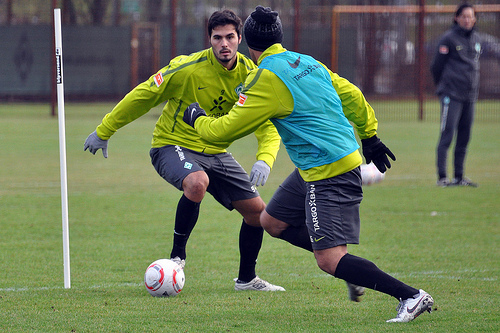
\includegraphics[width=\textwidth]{5369771639}
         \caption{Immagine originale}
     \end{subfigure}
     \begin{subfigure}[b]{0.45\textwidth}
         \centering
         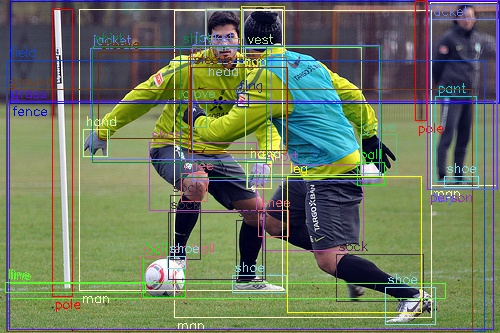
\includegraphics[width=\textwidth]{5369771639_detection.jpg}
         \caption{Object Detection}
     \end{subfigure}
     \begin{subfigure}[b]{0.45\textwidth}
         \centering
         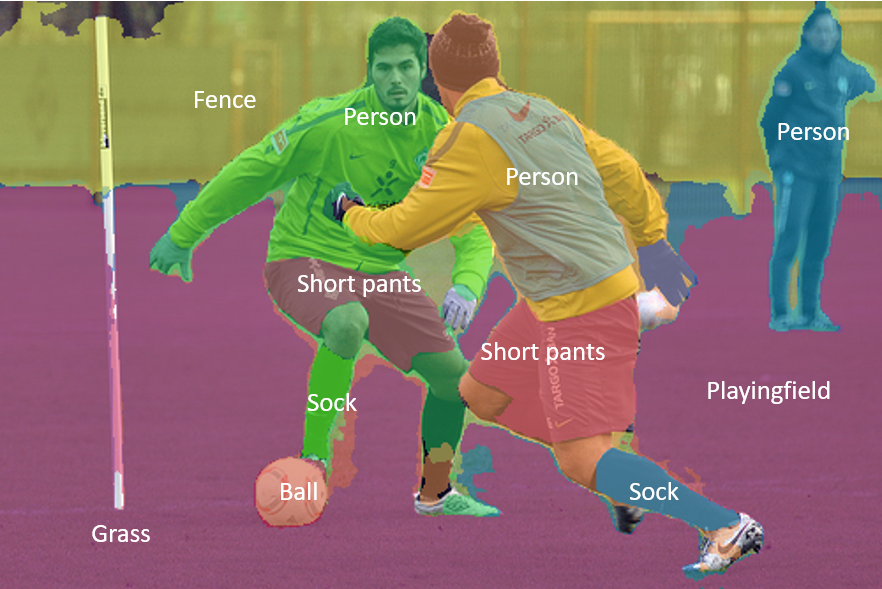
\includegraphics[width=\textwidth]{5369771639_seg}
         \caption{Image Segmentation}
     \end{subfigure}
     \captionsetup{singlelinecheck=off}
        \caption{Illustrazione contenente i risultati delle componenti di image understanding per l'immagine di Flickr30k con id: \textit{5369771639}.
        Caption di riferimento: 1) Two male soccer players in lime green uniforms passing the ball to each other; 2) Two men on opposing teams are playing soccer in a field; 3) Two soccer players going head-to-head for a soccer ball; 4) Two men scrimmage in soccer, as a referee looks on; 5) Two soccer players in long sleeves.\\
        Di seguito vengono riportate le predizioni ottenute in ogni prova effettuata.\\
        \textbf{\acrshort{oscar}$_+$ \acrshort{mtl} seg1*}: \textit{two young men are playing soccer on a field}.\\
        \textbf{\acrshort{oscar}$_+$ \acrshort{scst} seg1*}: \textit{two soccer players, one in green and one in blue, are playing soccer}.\\
        \textbf{\acrshort{oscar}$_+$ \acrshort{mtl} seg2*}: \textit{two men are playing soccer on a field}.\\
        \textbf{\acrshort{oscar}$_+$ \acrshort{scst} seg2*}: \textit{two men are playing soccer on a field}.\\
        \textbf{\acrshort{oscar}$_+$ \acrshort{mtl} seg3*}: \textit{two men playing soccer on a field}.\\
        \textbf{\acrshort{oscar}$_+$ \acrshort{scst} seg3*}: \textit{two men are playing soccer on a field}.\\
        \textbf{\acrshort{oscar}$_+$ \acrshort{mtl} seg+det1*}: \textit{two soccer players in yellow and blue uniforms are playing soccer}.\\
        \textbf{\acrshort{oscar}$_+$ \acrshort{scst} seg+det1*}: \textit{two soccer players in yellow are playing a game}.\\
        \textbf{\acrshort{oscar}$_+$ \acrshort{mtl} seg+det2*}: \textit{two men playing soccer on a field}.\\
        \textbf{\acrshort{oscar}$_+$ \acrshort{scst} seg+det2*}: \textit{two men in yellow shirts are playing soccer on a field}.\\
        \textbf{\acrshort{oscar}$_+$ \acrshort{mtl} seg+det3*}: \textit{two soccer players in yellow and blue uniforms are playing soccer}.\\
        \textbf{\acrshort{oscar}$_+$ \acrshort{scst} seg+det3*}: \textit{two men in yellow and blue uniforms are playing soccer}.\\
        \textbf{\acrshort{oscar}$_+$ \acrshort{mtl} det*}: \textit{two men in yellow and blue uniforms playing soccer}.\\
        \textbf{\acrshort{oscar}$_+$ \acrshort{scst} det*}: \textit{two men in yellow and blue uniforms are playing soccer}.
        }
        \label{fig:test1}
\end{figure}

\begin{figure}[H]
     \centering
     \begin{subfigure}[b]{0.32\textwidth}
         \centering
         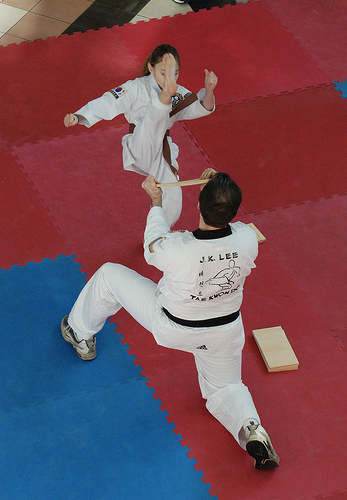
\includegraphics[width=\textwidth]{101362133}
         \caption{Immagine originale}
     \end{subfigure}
     \begin{subfigure}[b]{0.32\textwidth}
         \centering
         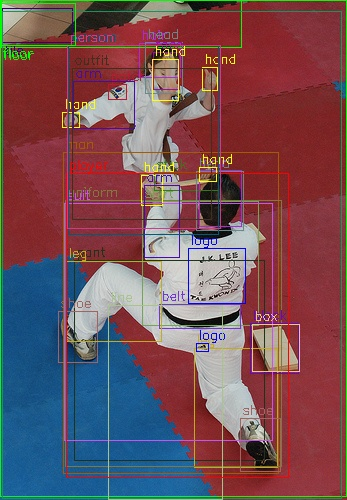
\includegraphics[width=\textwidth]{101362133_detection.jpg}
         \caption{Object Detection}
     \end{subfigure}
     \begin{subfigure}[b]{0.32\textwidth}
         \centering
         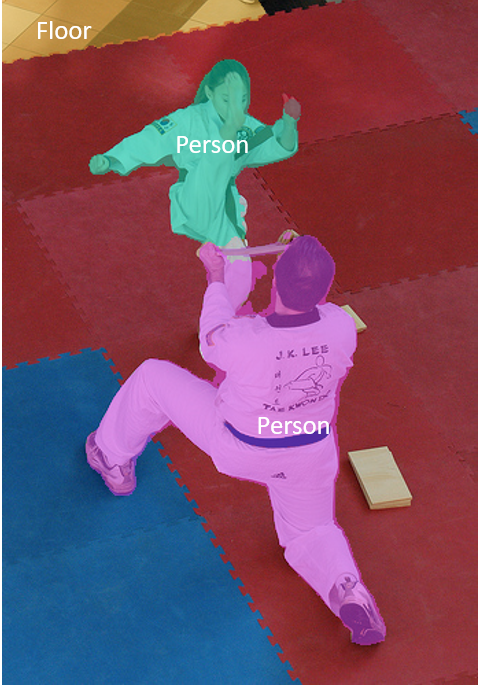
\includegraphics[width=\textwidth]{101362133_seg}
         \caption{Image Segmentation}
     \end{subfigure}
     \captionsetup{singlelinecheck=off}
        \caption{Illustrazione contenente i risultati delle componenti di image understanding per l'immagine di Flickr30k con id: \textit{101362133}.
        Caption di riferimento: 1) A young female student performing a downward kick to break a board held by her Karate instructor; 2) Girl about to kick a piece of wood in half while karate instructor holds it; 3) A girl kicking a stick that a man is holding in tae kwon do class; 4) A girl in karate uniform breaking a stick with a front kick; 5) A girl breaking boards by using karate.\\
        Di seguito vengono riportate le predizioni ottenute in ogni prova effettuata.\\
        \textbf{\acrshort{oscar}$_+$ \acrshort{mtl} seg1*}: \textit{two men are competing in a martial arts match}.\\
        \textbf{\acrshort{oscar}$_+$ \acrshort{scst} seg1*}: \textit{two men are performing a martial arts move on the floor}.\\
        \textbf{\acrshort{oscar}$_+$ \acrshort{mtl} seg2*}: \textit{two men are competing in a martial arts match}.\\
        \textbf{\acrshort{oscar}$_+$ \acrshort{scst} seg2*}: \textit{two men are performing a martial arts move on the floor}.\\
        \textbf{\acrshort{oscar}$_+$ \acrshort{mtl} seg3*}: \textit{two men, one in a white shirt and one in a black shirt, are fighting}.\\
        \textbf{\acrshort{oscar}$_+$ \acrshort{scst} seg3*}: \textit{two young men are practicing martial arts on the floor}.\\
        \textbf{\acrshort{oscar}$_+$ \acrshort{mtl} seg+det1*}: \textit{two people are practicing martial arts on a red mat}.\\
        \textbf{\acrshort{oscar}$_+$ \acrshort{scst} seg+det1*}: \textit{two people are practicing martial arts on a red mat}.\\
        \textbf{\acrshort{oscar}$_+$ \acrshort{mtl} seg+det2*}: \textit{two people are practicing martial arts on a red mat}.\\
        \textbf{\acrshort{oscar}$_+$ \acrshort{scst} seg+det2*}: \textit{two people are practicing martial arts on a red mat}.\\
        \textbf{\acrshort{oscar}$_+$ \acrshort{mtl} seg+det3*}: \textit{two people are practicing martial arts on a red mat}.\\
        \textbf{\acrshort{oscar}$_+$ \acrshort{scst} seg+det3*}: \textit{two people are practicing martial arts on a red mat}.\\
        \textbf{\acrshort{oscar}$_+$ \acrshort{mtl} det*}: \textit{two people are practicing martial arts on a red mat}.\\
        \textbf{\acrshort{oscar}$_+$ \acrshort{scst} det*}: \textit{two people are practicing martial arts on a red mat}.
        }
        \label{fig:test2}
\end{figure}


\begin{figure}[H]
     \centering
     \begin{subfigure}[b]{0.31\textwidth}
         \centering
         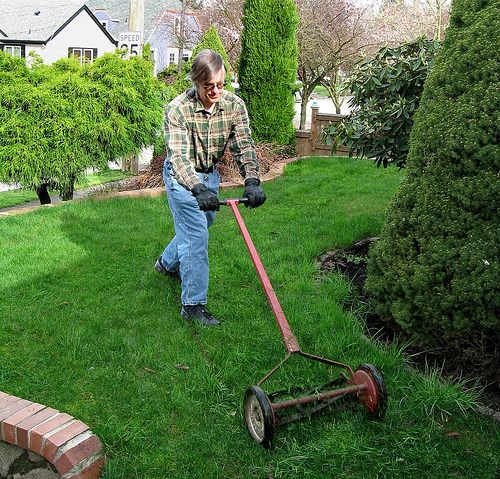
\includegraphics[width=\textwidth]{4434125934}
         \caption{Immagine originale}
     \end{subfigure}
     \begin{subfigure}[b]{0.31\textwidth}
         \centering
         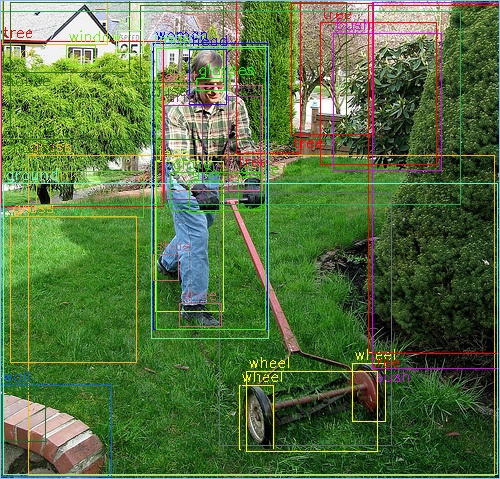
\includegraphics[width=\textwidth]{4434125934_detection.jpg}
         \caption{Object Detection}
     \end{subfigure}
     \begin{subfigure}[b]{0.31\textwidth}
         \centering
         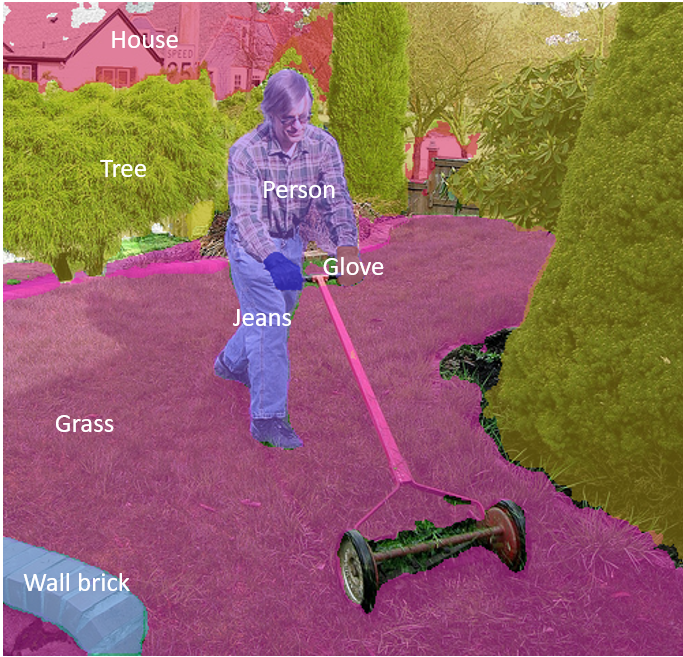
\includegraphics[width=\textwidth]{4434125934_seg}
         \caption{Image Segmentation}
     \end{subfigure}
     \captionsetup{singlelinecheck=off}
        \caption{Illustrazione contenente i risultati delle componenti di image understanding per l'immagine di Flickr30k con id: \textit{4434125934}.
        Caption di riferimento: 1)  A man, dressed in bright blue jeans and a plaid shirt, mows a shaggy green lawn in his cozy suburban front yard; 2) A guy maintains his yard by mowing with a traditional, non-powered lawn mower; 3) A gray-haired man wearing black gloves is moving the lawn; 4) A man mows a small lawn with a push mower; 5) Man in long-sleeve shirt mows his lawn.\\
        Di seguito vengono riportate le predizioni ottenute in ogni prova effettuata.\\
        \textbf{\acrshort{oscar}$_+$ \acrshort{mtl} seg1*}: \textit{a man in a blue shirt is using a chainsaw to cut down a tree}.\\
        \textbf{\acrshort{oscar}$_+$ \acrshort{scst} seg1*}: \textit{a man in a blue shirt is working on a garden}.\\
        \textbf{\acrshort{oscar}$_+$ \acrshort{mtl} seg2*}: \textit{a man in a blue shirt and jeans is digging a hole with a shovel}.\\
        \textbf{\acrshort{oscar}$_+$ \acrshort{scst} seg2*}: \textit{a man in a green shirt is working on a garden}.\\
        \textbf{\acrshort{oscar}$_+$ \acrshort{mtl} seg3*}: \textit{a man in a blue shirt and jeans is digging a hole with a shovel}.\\
        \textbf{\acrshort{oscar}$_+$ \acrshort{scst} seg3*}: \textit{a man in a blue shirt is working on a piece of garden}.\\
        \textbf{\acrshort{oscar}$_+$ \acrshort{mtl} seg+det1*}: \textit{a man in a plaid shirt is mowing the grass with a red mower}.\\
        \textbf{\acrshort{oscar}$_+$ \acrshort{scst} seg+det1*}: \textit{a man in a plaid shirt is mowing the grass with a red mower}.\\
        \textbf{\acrshort{oscar}$_+$ \acrshort{mtl} seg+det2*}: \textit{a woman in a plaid shirt is mowing the grass with a red mower}.\\
        \textbf{\acrshort{oscar}$_+$ \acrshort{scst} seg+det2*}: \textit{a man in a plaid shirt is cutting grass with a red mower}.\\
        \textbf{\acrshort{oscar}$_+$ \acrshort{mtl} seg+det3*}: \textit{a man in a plaid shirt and jeans is mowing a lawn with a red mower}.\\
        \textbf{\acrshort{oscar}$_+$ \acrshort{scst} seg+det3*}: \textit{a man in a plaid shirt and jeans is mowing the lawn with a red mower}.\\
        \textbf{\acrshort{oscar}$_+$ \acrshort{mtl} det*}: \textit{a man in a plaid shirt and blue jeans is mowing the lawn}.\\
        \textbf{\acrshort{oscar}$_+$ \acrshort{scst} det*}: \textit{a man in a plaid shirt is mowing the lawn with a red mower}.
        }
        \label{fig:test3}
\end{figure}

\begin{figure}[H]
     \centering
     \begin{subfigure}[b]{0.45\textwidth}
         \centering
         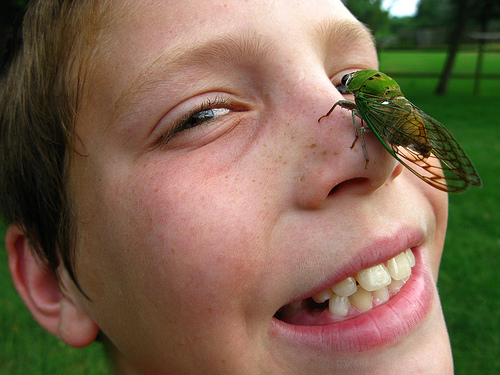
\includegraphics[width=\textwidth]{2750185692}
         \caption{Immagine originale}
     \end{subfigure}
     \begin{subfigure}[b]{0.45\textwidth}
         \centering
         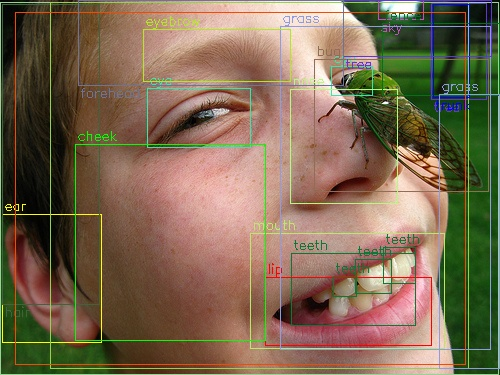
\includegraphics[width=\textwidth]{2750185692_detection.jpg}
         \caption{Object Detection}
     \end{subfigure}
     \begin{subfigure}[b]{0.45\textwidth}
         \centering
         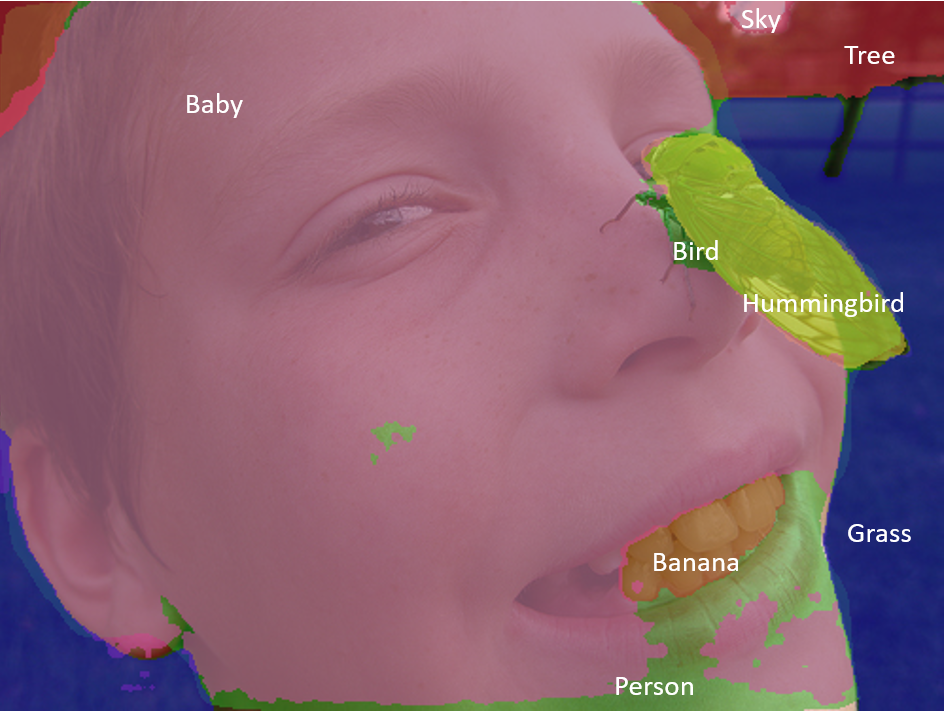
\includegraphics[width=\textwidth]{2750185692_seg}
         \caption{Image Segmentation}
     \end{subfigure}
     \captionsetup{singlelinecheck=off}
        \caption{Illustrazione contenente i risultati delle componenti di image understanding per l'immagine di Flickr30k con id: \textit{2750185692}.
        Caption di riferimento: 1) Young boy smiles as an extremely large kelly green fly perches on his nose; 2) A green beetle is resting upon a freckled nose of a young boy; 3) Boy that is outside with a green bug sitting on his nose; 4) A boy poses with a large green insect on his nose; 5) A boy with a winged bug perched on his nose.\\
        Di seguito vengono riportate le predizioni ottenute in ogni prova effettuata.\\
        \textbf{\acrshort{oscar}$_+$ \acrshort{mtl} seg1*}: \textit{a man in a green shirt is holding a large bird}.\\
        \textbf{\acrshort{oscar}$_+$ \acrshort{scst} seg1*}: \textit{a man is holding a green bird in a tree}.\\
        \textbf{\acrshort{oscar}$_+$ \acrshort{mtl} seg2*}: \textit{a young boy is eating a banana}.\\
        \textbf{\acrshort{oscar}$_+$ \acrshort{scst} seg2*}: \textit{a young boy is holding a bird in his mouth}.\\
        \textbf{\acrshort{oscar}$_+$ \acrshort{mtl} seg3*}: \textit{a young boy is eating a banana}.\\
        \textbf{\acrshort{oscar}$_+$ \acrshort{scst} seg3*}: \textit{a young boy is holding a bird in his hand}.\\
        \textbf{\acrshort{oscar}$_+$ \acrshort{mtl} seg+det1*}: \textit{a young boy is looking at a hummingbird}.\\
        \textbf{\acrshort{oscar}$_+$ \acrshort{scst} seg+det1*}: \textit{a young boy is looking at a hummingbird}.\\
        \textbf{\acrshort{oscar}$_+$ \acrshort{mtl} seg+det2*}: \textit{a young boy is looking at a green insect}.\\
        \textbf{\acrshort{oscar}$_+$ \acrshort{scst} seg+det2*}: \textit{a young boy is looking at a green bug}.\\
        \textbf{\acrshort{oscar}$_+$ \acrshort{mtl} seg+det3*}: \textit{a young boy with a green butterfly on his nose}.\\
        \textbf{\acrshort{oscar}$_+$ \acrshort{scst} seg+det3*}: \textit{a young boy is looking at a green insect on his nose}.\\
        \textbf{\acrshort{oscar}$_+$ \acrshort{mtl} det*}: \textit{a young boy is looking at a green insect}.\\
        \textbf{\acrshort{oscar}$_+$ \acrshort{scst} det*}: \textit{a young boy is looking at a green insect on his nose}.
        }
        \label{fig:test4}
\end{figure}

\begin{figure}[H]
     \centering
     \begin{subfigure}[b]{0.47\textwidth}
         \centering
         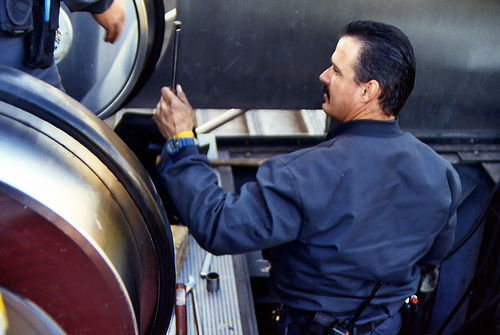
\includegraphics[width=\textwidth]{1989609}
         \caption{Immagine originale}
     \end{subfigure}
     \begin{subfigure}[b]{0.47\textwidth}
         \centering
         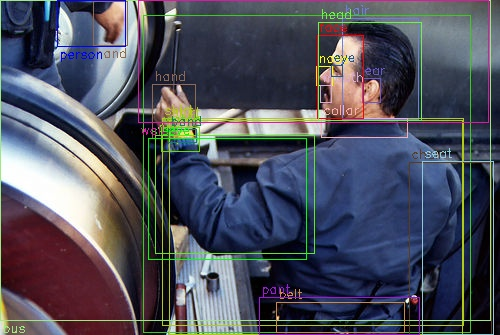
\includegraphics[width=\textwidth]{1989609_detection.jpg}
         \caption{Object Detection}
     \end{subfigure}
     \begin{subfigure}[b]{0.47\textwidth}
         \centering
         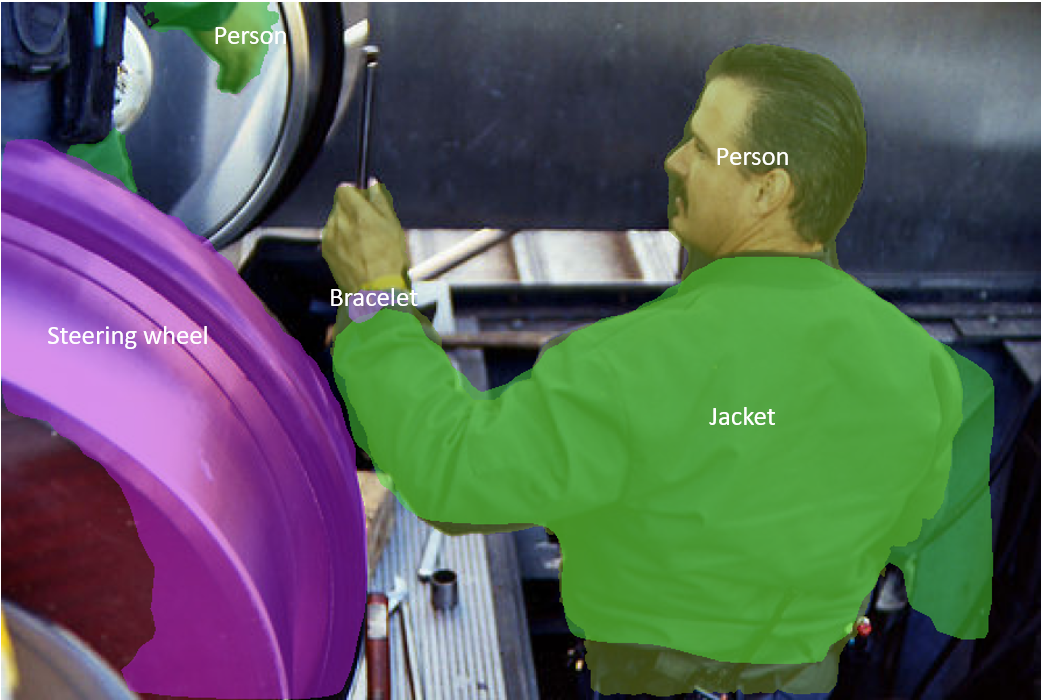
\includegraphics[width=\textwidth]{1989609_seg}
         \caption{Image Segmentation}
     \end{subfigure}
     \captionsetup{singlelinecheck=off}
        \caption{Illustrazione contenente i risultati delle componenti di image understanding per l'immagine di Flickr30k con id: \textit{1989609}.
        Caption di riferimento: 1) A man wearing blue coveralls is handing a tool to another person; 2) A man in a navy blue jacket holding a tool in his dirty hand; 3) A man in a work uniform passing a tool to another person; 4) Man in a blue jumpsuit attempts to repair an escalator; 5) A man with a mustache works on a broken escalator.\\
        Di seguito vengono riportate le predizioni ottenute in ogni prova effettuata.\\
        \textbf{\acrshort{oscar}$_+$ \acrshort{mtl} seg1*}: \textit{a man in a blue jacket is driving a car}.\\
        \textbf{\acrshort{oscar}$_+$ \acrshort{scst} seg1*}: \textit{a man in a blue jacket is driving a car}.\\
        \textbf{\acrshort{oscar}$_+$ \acrshort{mtl} seg2*}: \textit{a man in a blue jacket is driving a car}.\\
        \textbf{\acrshort{oscar}$_+$ \acrshort{scst} seg2*}: \textit{a man in a black jacket is driving a car}.\\
        \textbf{\acrshort{oscar}$_+$ \acrshort{mtl} seg3*}: \textit{a man in a blue jacket is driving a car}.\\
        \textbf{\acrshort{oscar}$_+$ \acrshort{scst} seg3*}: \textit{a man in a blue jacket is driving a car}.\\
        \textbf{\acrshort{oscar}$_+$ \acrshort{mtl} seg+det1*}: \textit{a man in a blue jacket is working on a car}.\\
        \textbf{\acrshort{oscar}$_+$ \acrshort{scst} seg+det1*}: \textit{a man in a blue jacket is standing at the wheel of a car}.\\
        \textbf{\acrshort{oscar}$_+$ \acrshort{mtl} seg+det2*}: \textit{a man in a blue jacket is working on a car}.\\
        \textbf{\acrshort{oscar}$_+$ \acrshort{scst} seg+det2*}: \textit{a man in a blue jacket is working on a car}.\\
        \textbf{\acrshort{oscar}$_+$ \acrshort{mtl} seg+det3*}: \textit{a man in a blue jacket is working on a car}.\\
        \textbf{\acrshort{oscar}$_+$ \acrshort{scst} seg+det3*}: \textit{a man in a blue jacket is working on a car}.\\
        \textbf{\acrshort{oscar}$_+$ \acrshort{mtl} det*}: \textit{a man in a blue shirt is working on a car}.\\
        \textbf{\acrshort{oscar}$_+$ \acrshort{scst} det*}: \textit{a man in a blue shirt is working on a car}.
        }
        \label{fig:test5}
\end{figure}

\begin{figure}[H]
     \centering
     \begin{subfigure}[b]{0.32\textwidth}
         \centering
         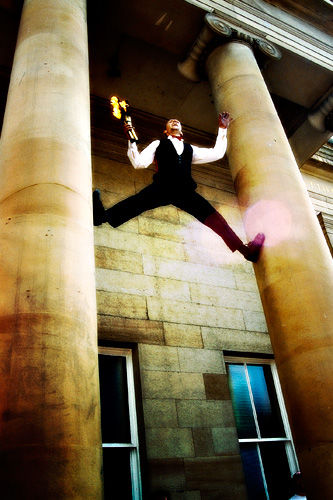
\includegraphics[width=\textwidth]{21138719}
         \caption{Immagine originale}
     \end{subfigure}
     \begin{subfigure}[b]{0.32\textwidth}
         \centering
         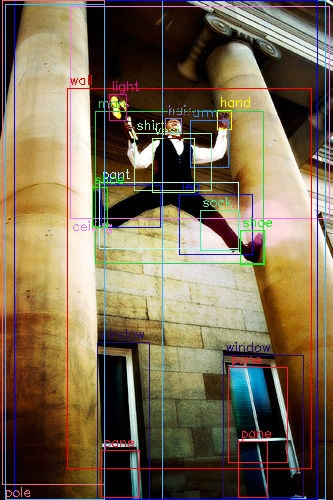
\includegraphics[width=\textwidth]{21138719_detection.jpg}
         \caption{Object Detection}
     \end{subfigure}
     \begin{subfigure}[b]{0.32\textwidth}
         \centering
         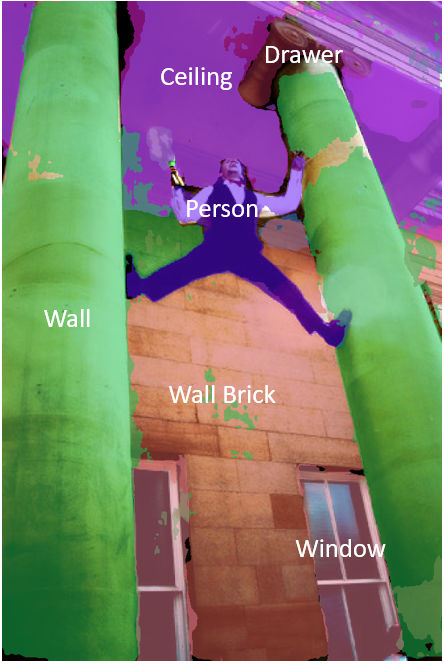
\includegraphics[width=\textwidth]{21138719_seg}
         \caption{Image Segmentation}
     \end{subfigure}
     \captionsetup{singlelinecheck=off}
        \caption{Illustrazione contenente i risultati delle componenti di image understanding per l'immagine di Flickr30k con id: \textit{21138719}.
        Caption di riferimento: 1) Man in black pants and vest balances between to pillars, holding two flaming torches in his right hand; 2) A well-dressed man climbing between two columns while holding torches; 3) A man in a suit is straddling two pillars while holding a flame; 4) Juggler standing balanced between two columns; 5) Man scaling wall with fire in hand.\\
        Di seguito vengono riportate le predizioni ottenute in ogni prova effettuata.\\
        \textbf{\acrshort{oscar}$_+$ \acrshort{mtl} seg1*}: \textit{a man in a black shirt is jumping in the air}.\\
        \textbf{\acrshort{oscar}$_+$ \acrshort{scst} seg1*}: \textit{a man in a black shirt is jumping in the air in a room}.\\
        \textbf{\acrshort{oscar}$_+$ \acrshort{mtl} seg2*}: \textit{a man in a black shirt is jumping in the air on a trampoline}.\\
        \textbf{\acrshort{oscar}$_+$ \acrshort{scst} seg2*}: \textit{a man in a black shirt is jumping on a ladder}.\\
        \textbf{\acrshort{oscar}$_+$ \acrshort{mtl} seg3*}: \textit{a man in a black shirt is jumping in the air on a trampoline}.\\
        \textbf{\acrshort{oscar}$_+$ \acrshort{scst} seg3*}: \textit{a man in a white shirt is jumping in the air on a ladder}.\\
        \textbf{\acrshort{oscar}$_+$ \acrshort{mtl} seg+det1*}: \textit{a man is hanging upside down from a rope}.\\
        \textbf{\acrshort{oscar}$_+$ \acrshort{scst} seg+det1*}: \textit{a man in a black shirt is hanging from a pipe}.\\
        \textbf{\acrshort{oscar}$_+$ \acrshort{mtl} seg+det2*}: \textit{a man is hanging upside down from a rope}.\\
        \textbf{\acrshort{oscar}$_+$ \acrshort{scst} seg+det2*}: \textit{a man is hanging upside down from a building}.\\
        \textbf{\acrshort{oscar}$_+$ \acrshort{mtl} seg+det3*}: \textit{a man is jumping in the air between two columns}.\\
        \textbf{\acrshort{oscar}$_+$ \acrshort{scst} seg+det3*}: \textit{a man in a black suit is jumping between two columns}.\\
        \textbf{\acrshort{oscar}$_+$ \acrshort{mtl} det*}: \textit{a man is jumping in the air between two columns}.\\
        \textbf{\acrshort{oscar}$_+$ \acrshort{scst} det*}: \textit{a man in a black suit is jumping between two columns}.
        }
        \label{fig:test6}
\end{figure}
\newpage

\section{Considerazioni}\label{considerazioni}
I modelli ottenuti tramite la componente di Image Segmentation hanno ottenuto le performance più basse, però come si è visto nella Sezione \ref{analisi_qualitativa} sono stati in grado di produrre didascalie di discreta qualità dove è comunque comprensibile il contenuto visivo dell'immagine. Inoltre, come si è potuto vedere dai risultati il fine-tuning tramite \acrshort{scst} è molto utile, poichè permette di ottenere delle didascalie di qualità superiore. 


Analizzando l'andamento della loss function dei modelli che usano l'ensemble di Image Segmentation è stata osservata una discesa più accentuata rispetto alla versione che usa i modelli di Object Detection. Infatti, è stata effettuata una prova in cui sono stati allenati i modelli con alcune epoche aggiuntive e sono stati notati dei miglioramenti più marcati nella versione che usa la segmentazione. Quest'ultima osservazione non è stata applicata su tutti i modelli per effettuare delle comparazioni eque, che considerano gli stessi parametri per tutte le prove, e perché il fine-tuning dei modelli richiede molto tempo (basti pensare che ogni fine-tuning effettuato ha richiesto più di sei giorni per il completamento).


Le prove che prevedono la componente di Image Segmentation (da sola o in combinazione, ad eccezione della prova seg+det3) hanno ottenuto dei risultati bassi sulla metrica \acrshort{bleu}@4. La principale motivazione deriva dal fatto che questa metrica si basa sulla precisione dei termini utilizzati, molto spesso le classi individuate tramite segmentazione sono poco accurate e le caption prodotte contengono termini più generici e sinonimi.
Inoltre, la combinazione tra tutte le feature estratte tramite Image Segmentation con tutte quelle estratte tramite Object Detection ha ottenute le performance più elevate su tre metriche ad eccezione della \acrshort{cider}. Analizzando le didascalie prodotte non è stata trovata una grossa differenza ad eccezione di qualche dettaglio (per esempio la Figura \ref{fig:test5}), poichè la differenza è minima è stato difficile trovare la possibile causa.

Infine, una cosa molto importate da considerare è che spesso le caption generate non sono molto fedeli a quelle di riferimento, questo è dovuto principalmente al fatto che le didascalie di riferimento contengono informazioni implicite, contestuali e altri aspetti difficili da catturare considerando solo gli oggetti presenti nell'immagine.
\chapter{Conclusioni}
In questa tesi magistrale sono stati esplorati i progressi dell'Image Captioning soffermandosi principalmente sulla componente di image understanding con l'obiettivo di sviluppare un prototipo che cercasse di migliorare la comprensione dell'immagine.


Nella Sezione \ref{obiettivo} sono state poste le seguenti domande di ricerca:
\begin{enumerate}[leftmargin=1.5cm,label=\textit{RQ\arabic*:},ref=\textit{RQ\arabic*}]
    \item\label{rq_1}\textit{Com'è possibile migliorare la componente di image understanding nelle tecniche di Image Captioning dello stato dell'arte?}
    \item\label{rq_2}\textit{Come può essere implementata la componente di Image Segmentation?}
    \item\label{rq_3}\textit{Come può essere migliorata la componente di Image Segmentation?}
    \item\label{rq_4}\textit{Come si comporta \acrshort{oscar}$_+$ con gli oggetti segmentati?}
    \item\label{rq_5}\textit{Quali sono i benefici dell'uso dell'Image Segmentation nei modelli di Image Captioning dello stato dell'arte?}
\end{enumerate}


Inizialmente è stato studiato lo stato dell'arte degli approcci di Image Captioning, osservando che gli approcci di generazione diretta delle didascalie basati sui modelli di Object Detection e sui modelli linguistici siano i più popolari. Il modello di Object Detection utilizzato è una variante di \acrshort{faster_rcnn} progettata appositamente per questa tipologia di task, la quale ha permesso il raggiungimento di performance allo stato dell'arte.
Tra i modelli linguistici è stato scelto un modello costruito su \acrshort{bert} chiamato \acrshort{oscar}$_+$, il quale è stato pre-addestrato su molti task composti da una componente visiva e da una componente linguistica. \acrshort{oscar}$_+$ è un modello generico che ha appreso rappresentazioni cross-modali e il suo fine-tuning sul compito specifico permette di ottenere risultati allo stato dell'arte.


In questa tesi sono state condotte alcune analisi sul modello di Object Detection selezionato e nonostante sia stato appositamente sviluppato per questa tipologia di task esistono diverse regioni, rappresentanti oggetti di classi diverse, codificate tramite feature molto simili. 
Infatti, le regioni visive estratte sono risultate spesso sovrapposte, rumorose e ambigue, questo inevitabilmente risulta in feature delle regioni meno significative. Pertanto, è stata posta la domanda di ricerca \ref{rq_1}. Quindi è stato condotto uno studio che cerca di risolvere questo problema. La soluzione identificata prevede un approccio innovativo che sfrutta il task di Image Segmentation nella componente di image understanding. In questa tesi è stata scelta questa soluzione perché l'Image Segmentation per ogni istanza oltre a predire il tag e la bounding box predice anche una maschera binaria, la quale consente di segmentare l'oggetto rimuovendo il rumore.


Nello stato dell'arte non sono stati trovati approcci che sfruttano dei modelli di segmentazione progettati appositamente per questa tipologia di task. Pertanto, è stata posta la domanda di ricerca \ref{rq_2} e in questa tesi è stato implementato un approccio di segmentazione che prevede l'utilizzo di due modelli di segmentazione già addestrati con ottime performance. Nel dettaglio si tratta del modello \acrshort{detr} di Panoptic Segmentation allenato su \acrshort{coco} Panoptic e di una \acrshort{mask_rcnn} di Instance Segmentation allenata su \acrshort{lvis}.


L'ensemble dei modelli di segmentazione riesce a predire meno classi rispetto al modello di Object Detection utilizzato e spesso oggetti molto importanti, che sono imprescindibili per la comprensione del contenuto visivo e per la generazione della caption, non vengono rilevati. Inoltre, l'ensemble dei modelli di segmentazione a volte ha difficoltà nella predizione delle classi corrette.
Quindi è stata posta la domanda di ricerca \ref{rq_3}.
In questa tesi le risorse computazionali sono state limitate e i risultati dell'ensemble dei modelli di segmentazione sono stati migliorati tramite una pipeline che sfrutta le predizioni ottenute dal modello di Object Detection, includendo gli oggetti mancanti e correggendo le classi assegnate scorrettamente.
La soluzione migliore sarebbe stata quella di progettare un modello di segmentazione pensato appositamente per questa tipologia di task in grado di predire molte classi diverse con buone performance, utilizzando tecniche di data augmentation efficaci per gestire adeguatamente le classi sbilanciate e il bilanciamento dei dataset utilizzati.% (seguendo un approccio simile a quello utilizzato per definire il modello di Object Detection).

La risposta alle domande \ref{rq_4} e \ref{rq_5} è stata ottenuta utilizzando il dataset Flickr30K. 
Le immagini di questo dataset sono state processate utilizzando i vari approcci di image understanding implementati e le feature ottenute sono state utilizzate per effettuare il fine-tuning di \acrshort{oscar}$_+$ sul task di Image Captioning. I modelli fine-tuned ottenuti sono stati testati sullo split di test utilizzando varie metriche, le quali consentono di catturare caratteristiche linguistiche differenti.

Analizzando i risultati è emerso che le sole feature ottenute tramite l'ensemble dei modelli di segmentazione non sono sufficienti per ottenere performance superiori rispetto al modello linguistico fine-tuned tramite Object Detection, poichè spesso non vengono rilevati oggetti importanti presenti nelle didascalie di riferimento. Tramite un'analisi qualitativa sono stati compresi meglio i risultati ed è stata trovata una risposta alla domanda \ref{rq_4}. Dall'analisi è emerso che nelle immagini in cui tutti gli oggetti più importanti vengono rilevati si ottengono didascalie di buona qualità. 
La combinazione tra Image Segmentation e Object Detection ha permesso alla segmentazione di ottenere miglioramenti significativi nelle prestazioni. Quindi è sembrato che \acrshort{oscar}$_+$ sia in grado di utilizzare correttamente anche gli oggetti segmentati.


La prova composta da tutte le feature estratte sia tramite l'Image Segmentation che tramite l'Object Detection ha ottenuto le performance più elevate superando leggermente quelle ottenute tramite la sola Object Detection, poichè su tre delle quattro metriche di valutazione utilizzate ha ottenuto i risultati migliori. Quindi, questo risultato ha permesso di rispondere alla domanda \ref{rq_5}, dimostrando che l'inclusione dell'Image Segmentation porta dei benefici ai modelli di Image Captioning dello stato dell'arte su alcune metriche di valutazione. Inoltre, valutando qualitativamente alcune immagini è stata notata nelle didascalie ottenute la presenza di alcuni dettagli non catturati con la sola Object Detection.
Nonostante abbia migliorato leggermente le performance ha anche complicato notevolmente la fase di estrazione delle feature aumentandone il tempo necessario.


Le domande \ref{rq_4} e \ref{rq_5} avrebbero bisogno di un modello di segmentazione robusto progettato per questa tipologia di task, in grado di predire molti oggetti di classi diverse con buone performance, per trovare delle risposte più esaustive.
\chapter{Sviluppi Futuri}
In questo capitolo viene fornita una lista dei lavori futuri che vengono considerati utili per migliorare questo progetto:
\begin{enumerate}
    \item Implementazione di un modello di Image Segmentation costruito appositamente per task che prevedono coppie immagine-testo. Questo modello può essere progettato seguendo tre strategie differenti:
    \begin{enumerate}
        \item Instance Segmentation: il modello viene costruito sfruttando i dataset di Instance Segmentation più appropriati per questi task, attualmente i dataset disponibili più interessanti risultato: \acrshort{coco} \cite{lin2014microsoft}, \acrshort{lvis} \cite{gupta2019lvis}, ADE20K \cite{zhou2017scene} (prestando attenzione agli oggetti di tipo stuff) e OpenImages \cite{OpenImages}. Tramite questi dataset non vengono catturati gli oggetti di tipo stuff poichè risultano più difficili da identificare per un modello di Instance Segmentation. Pertanto, si dovrebbe utilizzare un modello che potrebbe essere in grado di localizzare questi oggetti, il quale considera anche il dataset \acrshort{coco} Stuff. Un modello molto interessante è \acrshort{mask_rcnn}, poichè è una variante di \acrshort{faster_rcnn} che si è comportata molto bene con questi oggetti nel task di Object Detection.
        Infine, il modello può essere reso robusto sfruttando tecniche di data augmentation molto interessanti come Copy-Paste\footnote{\url{https://github.com/tensorflow/tpu/tree/master/models/official/detection/projects/copy_paste}} \cite{ghiasi2020simple};
        \item Panoptic Segmentation: viene definito un nuovo dataset costruito dall'unione tra \acrshort{coco} Panoptic e \acrshort{lvis}, ridefinendo le maschere di segmentazione affinché non ci siano oggetti sovrapposti. Il dataset ottenuto viene utilizzato per allenare un modello di Panoptic Segmentation in grado di generare delle segmentazioni della scena ancora più ricche di oggetti rilevati. Infine, può essere utilizzato anche il dataset ADE20k che prevede sia oggetti di tipo stuff che thing;
        \item Combinazione tra Object Detection e Image Segmentation: il modello viene costruito tramite un paradigma di addestramento parzialmente supervisionato \cite{hu2018learning}. Questi paradigmi permettono di addestrare modelli di segmentazione su un grande insieme di classi che hanno tutte annotazioni di bounding box, ma solo una piccola frazione di esse ha le annotazioni delle maschere di segmentazione. Questa strategia risulta molto interessante perché i dataset di segmentazione consentono di riconoscere meno classi rispetto a quelle che si potrebbero rilevare tramite i dataset di Object Detection. Il modello utilizzato dovrebbe  decomporre il problema della segmentazione nei sottoprocessi di rilevamento degli oggetti tramite bounding box e previsione della maschera;
    \end{enumerate}
    \item Retrain di \acrshort{oscar}$_+$ su triple che considerano anche gli oggetti segmentati;
    \item Sviluppare modelli linguistici leggeri pre-addestrati su molti dataset che prevedono coppie immagine-testo, poiché quando si hanno poche risorse computazionali come in questa tesi sono richiesti molti giorni per il fine-tuning. Infatti, i fine-tuning eseguiti in questa tesi hanno richiesto più di sei giorni ed è stata usata la versione costruita su \acrshort{bert} base. Questi modelli più leggeri possono essere ottenuti tramite Knowledge Distillation \cite{fang2021compressing} e recentemente è stato sviluppato il modello MiniVLM \cite{wang2020minivlm}, del quale non è stato ancora reso disponibile il modello pre-addestrato;
    \item Migliorare la rappresentazione degli oggetti considerando le relazioni e le interazioni;
    \item Testare tecniche di data augmentation sui dataset di Image Captioning, sia sulle immagini che sulle didascalie;
\end{enumerate}


\bibliographystyle{ieeetr}

\bibliography{Bibliography}

\end{document}